\protect\hypertarget{_Hlk129432535}{}{}4 ano

\section{1. Representar quantidades}\label{muxf3dulo-1}

Habilidades da BNCC: EF04MA01, EF04MA02.

Habilidades do Saeb

- Escrever números racionais (naturais de até 6 ordens, representação
fracionária ou decimal finita até a ordem dos milésimos) em sua
representação por algarismos ou em língua materna ou associar o registro
numérico ao registro em língua materna.

- Identificar a ordem ocupada por um algarismo ou seu valor posicional
(ou valor relativo) em um número natural de até 6 ordens.

- Comparar ou ordenar números racionais (naturais de até 6 ordens,
representação fracionária ou decimal finita até a ordem dos milésimos),
com ou sem suporte da reta numérica.

- Compor ou decompor números naturais de até 6 ordens na forma aditiva,
ou em suas ordens, ou em adições e multiplicações.

- Comparar diferentes sentenças de adições ou de subtrações de dois
números naturais.

- Determinar o número desconhecido que torna verdadeira uma igualdade
que envolve as operações fundamentais com números naturais de até 6
ordens.

\subsection{Conteúdo}\label{conteuxfado}

Neste módulo devemos revisar os conceitos de montagem de
números, frisando muito as classes e até a 6º ordem. E muito importante
os alunos terminarem o módulo sabendo o valor posicional e relativo de
cada algarismo quando estão em determinada ordem.

Além disso, trabalhar incansavelmente a decomposição dos números e a
escrita por extenso desses números.

%Produzir uma tabela igual à de baixo utilizando padrão de cores que o material seguirá

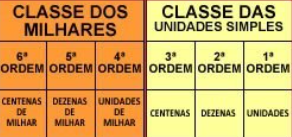
\includegraphics[width=3.55128in,height=1.66618in]{media/image1.png}

Valor posicional ou relativo: é o valor que o algarismo assume
dependendo da classe e da ordem em que ele está posicionado no número.

Exemplo: no número 352.146, o algarismo 5 apresenta valor posicional ou
relativo igual a 50.000, pois ocupa a 5º ordem, a qual está dentro da
classe dos milhares; ou seja, está na posição da dezena de milhar e,
sendo assim, 5 x 10.000 = 50.000.

Sistema de numeração Egípcio: era baseado em figuras; cada figura tinha um valor específico e a combinação entre figuras formava as qantidades e os valores que se desejava representar. 

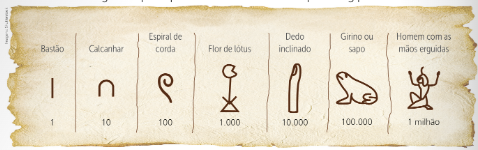
\includegraphics[width=3.98368in,height=1.25011in]{media/image2.png}

Sistema de numeração Maia: era baseado em representar
números com pontos e traços, conforme a figura.

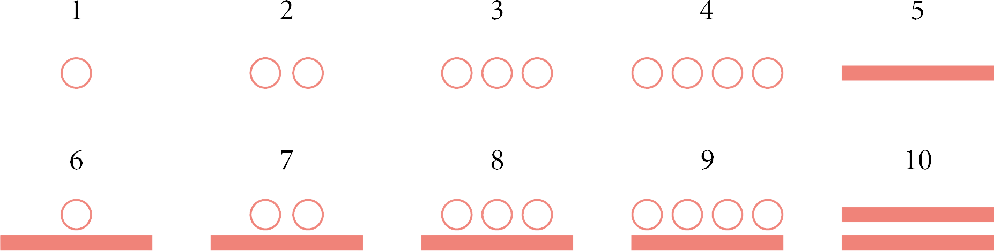
\includegraphics[width=2.66690in,height=0.81674in]{media/image3.png}

Sistema de numeração Romano: representava os números com letras
maiúsculas, seguindo regras específicas para essa representação.

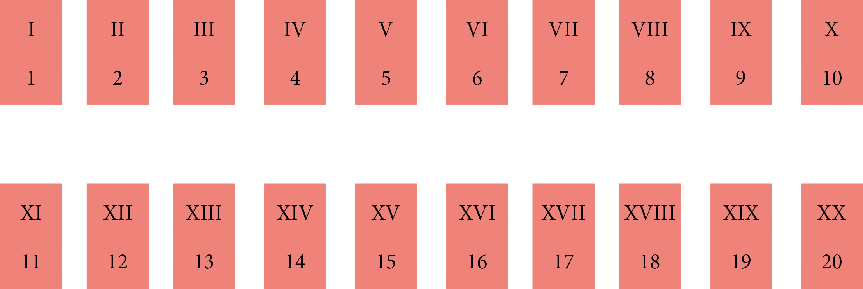
\includegraphics[width=3.97534in,height=1.23344in]{media/image4.png}

Sistema de numeração indo-arábico: é o utilizado por nós
até hoje e, com o passar do tempo, foi evoluindo na escrita dos algarismos e, consequentemente, dos números, como está representado na figura.

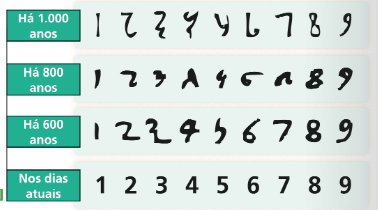
\includegraphics[width=3.15027in,height=1.75015in]{media/image5.png}

\subsection{Atividades}\label{atividades}

\subsubsection{1.}\label{section}

Escreva o valor posicional de cada algarismo
destacado -- ou seja, o valor que cada um assume de acordo com a posição
que ocupa no número.

\begin{enumerate}
\def\labelenumi{\alph{enumi})}
\item
  \textbf{8}24.345:
  O algarismo 8 destacado tem valor posicional igual a 800 000
  (oitocentos mil) já que se encontra na centena de milhar.
\item
  3\textbf{7}5.6\textbf{7}8:
  O primeiro algarismo 7 destacado tem valor posicional igual a 70 000
  (setenta mil) já que se encontra na dezena de milhar.
  Já o segundo algarismo 7 destacado tem valor posicional igual a 70
(setenta) já que está posicionado na dezena comum.
\item
  \textbf{1}48.52\textbf{1}:
  O primeiro algarismo 1 destacado tem valor posicional igual a 100 000
  (cem mil) já que se encontra na centena de milhar.
Já o segundo algarismo 1 destacado tem o valor posicional igual a 1 (uma
unidade) já que se encontra na unidade comum.

\subsubsection{2.}\label{section-1}

Decomponha os números a seguir de acordo com o valor posicional de cada
algarismo.

\begin{enumerate}
\def\labelenumi{\alph{enumi})}
\item
  32 084
\end{enumerate}

Deixar uma linha para resposta

\begin{enumerate}
\def\labelenumi{\alph{enumi})}
\item
  26 587
\end{enumerate}

Deixar uma linha para resposta

\begin{enumerate}
\def\labelenumi{\alph{enumi})}
\item
  2 105
\end{enumerate}

Deixar uma linha para resposta

Resposta:

\begin{enumerate}
\def\labelenumi{\alph{enumi})}
\item
  30 000 + 2 000 + 80 + 4 explore também a forma de escrever
\end{enumerate}

3 x 10 000 + 2 x 1 000 + 0 x 100 + 8 x 10 + 4. Além disso utilize o
exercício para treinar a escrita dos alunos. Exemplo trinta e dois mil e
oitenta e quatro.

\begin{enumerate}
\def\labelenumi{\alph{enumi})}
\item
  20 000 + 6 000 + 500 + 80 + 7 ou 2 x 10 000 + 6 x 1 000 + 5 x 100 + 8
  x 10 + 7
\item
  2 000 + 100 + 5 ou 2 x 1 000 + 1 x 100 + 0 x 10 + 5
\end{enumerate}

\subsubsection{3.}\label{section-2}

Monte os número compostos e registre-os nos locais correspondentes.

\begin{enumerate}
\def\labelenumi{\alph{enumi})}
\item
  7 unidades de milhar, 5 centenas e 4 unidades:
\end{enumerate}

deixar uma linha aqui na frente para resposta

\begin{enumerate}
\def\labelenumi{\alph{enumi})}
\item
  3 dezenas de milhar, 7 dezenas e 2 unidades:
\end{enumerate}

deixar uma linha aqui na frente para resposta

\begin{enumerate}
\def\labelenumi{\alph{enumi})}
\item
  9 centenas de milhar, 5 unidades de milhar e 6 centenas:
\end{enumerate}

deixar uma linha aqui na frente para resposta

\begin{enumerate}
\def\labelenumi{\alph{enumi})}
\item
  2 unidades de milhar, 6 centenas e 3 unidades:
\end{enumerate}

deixar uma linha aqui na frente para resposta

Resposta:

\begin{enumerate}
\def\labelenumi{\alph{enumi})}
\item
  7 504
\item
  30 072
\item
  905 600
\item
  2 603
\end{enumerate}

Professor devemos explorar bem essa volta pois muitos alunos desenvolvem
dificuldades, ou seja, sabem fazer a decomposição mas não compreendem a
volta.

\subsubsection{4.}\label{section-3}

Ligue os retângulos da coluna com 1 a um corresponde da coluna 2 que
represente a escrita por extenso do número indicado na primeira coluna.

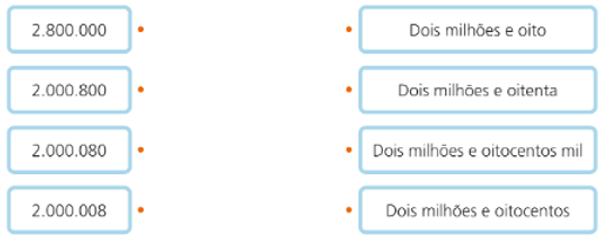
\includegraphics[width=3.55128in,height=1.46056in]{media/image7.png}

Produzir uma figura conforme a indicada acima trocando os números e
escritos dentro dos retângulos conforme indicado abaixo: (não colocar os
pontos em vermelho que aparecem na figura acima)

352 700 Trezentos e quatorze mil

200 015 Vinte mil e três

20 003 Trezentos e cinquenta e dois mil e setecentos

314 000 Duzentos mil e quinze

Resposta:

352 700 deve estar ligado ao trezentos e cinquenta e dois mil e
setecentos.

200 015 deve estar ligado ao duzentos mil e quinze.

20 003 deve estar ligado a vinte mil e três.

314 000 deve estar ligado ao trezentos e quatorze mil.

\subsubsection{5.}\label{section-4}

Alguns números foram escritos no sistema egípcio por Carlos. Utilize
seus conhecimentos e descubra quais números eles indicam em nosso
sistema de numeração.

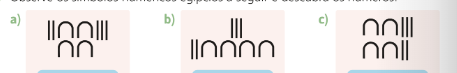
\includegraphics[width=3.80866in,height=0.60839in]{media/image8.png}

Construir uma figura dessa forma. As quantidades de cada figura importam
para a resolução.

Deixar 5 linhas para resposta

Resposta:

\begin{enumerate}
\def\labelenumi{\alph{enumi})}
\item
  4 x 10 + 5 x 1 = 45
\item
  4 x 10 + 5 x 1 = 45
\item
  4 x 10 + 5 x 1 = 45
\end{enumerate}

Professor converse com os alunos deixando claro que o sistema egípcio
não era posicional e sendo assim, a ordem da colocação dos desenhos não
importa e sim, a única coisa que importa é o valor atribuído a cada
figura.

\subsubsection{6.}\label{section-5}

André estava estudando os sistemas de numeração e por curiosidde quer
escrever cada um dos números abaixos no sistema de numeração egípcio.
Ajude ele nessa tarefa e, utilizando os símbolos egípcios, escreva cada
um dos números abaixo.

\begin{enumerate}
\def\labelenumi{\alph{enumi})}
\item
  120
\item
  535
\item
  1 240
\item
  12 132
\end{enumerate}

Deixar 8 linhas para resposta

Resposta:

\begin{enumerate}
\def\labelenumi{\alph{enumi})}
\item
  120
\end{enumerate}

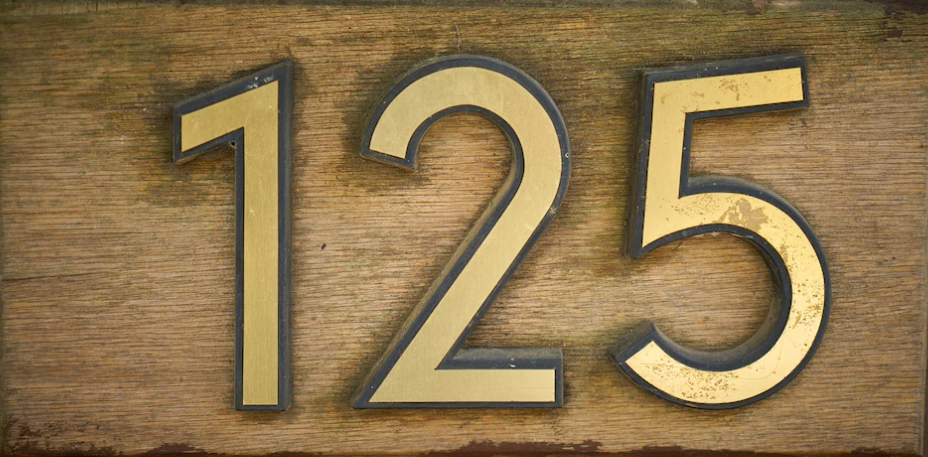
\includegraphics[width=0.37503in,height=0.40003in]{media/image9.png}
\includegraphics[width=0.38337in,height=0.31669in]{media/image10.png}
\includegraphics[width=0.38337in,height=0.31669in]{media/image10.png}

\begin{enumerate}
\def\labelenumi{\alph{enumi})}
\item
  535
\end{enumerate}

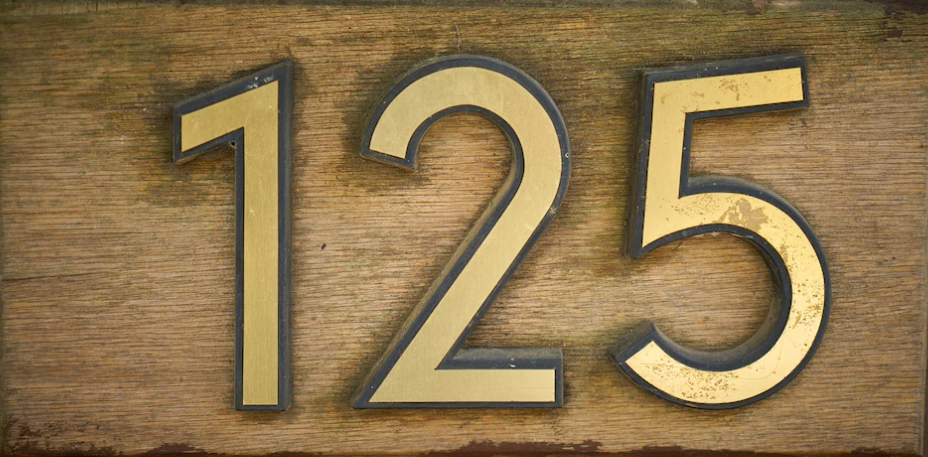
\includegraphics[width=0.37503in,height=0.40003in]{media/image9.png}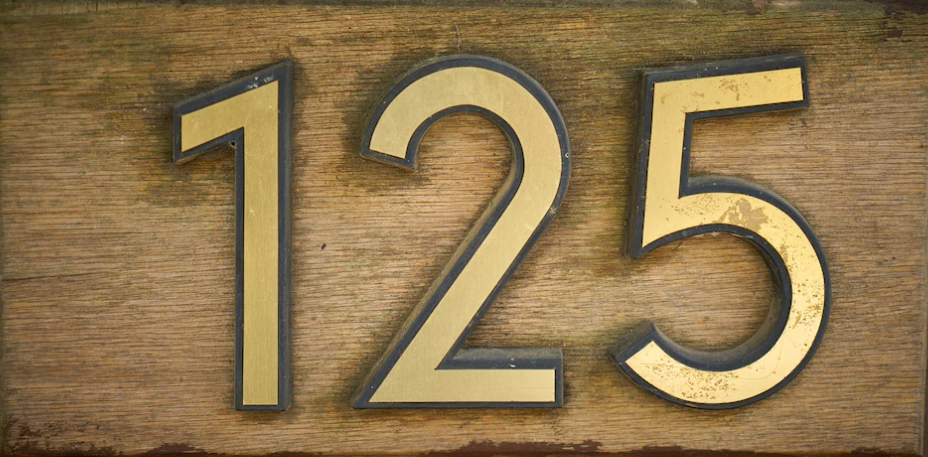
\includegraphics[width=0.37503in,height=0.40003in]{media/image9.png}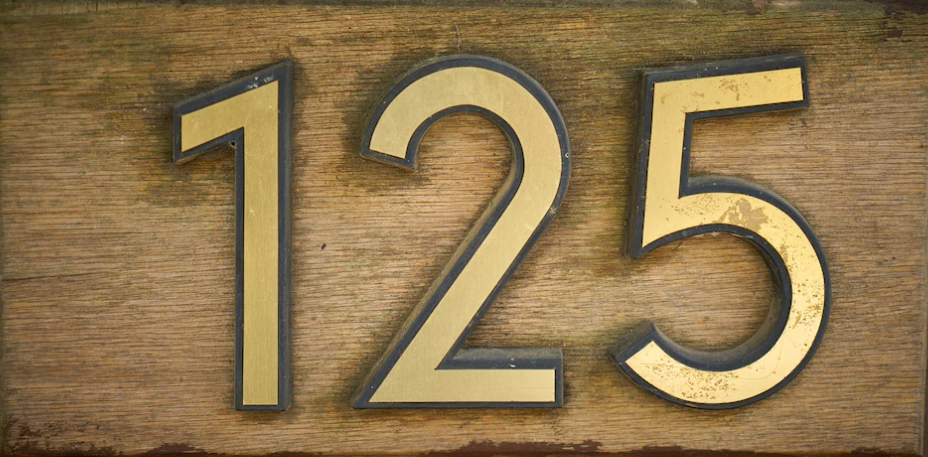
\includegraphics[width=0.37503in,height=0.40003in]{media/image9.png}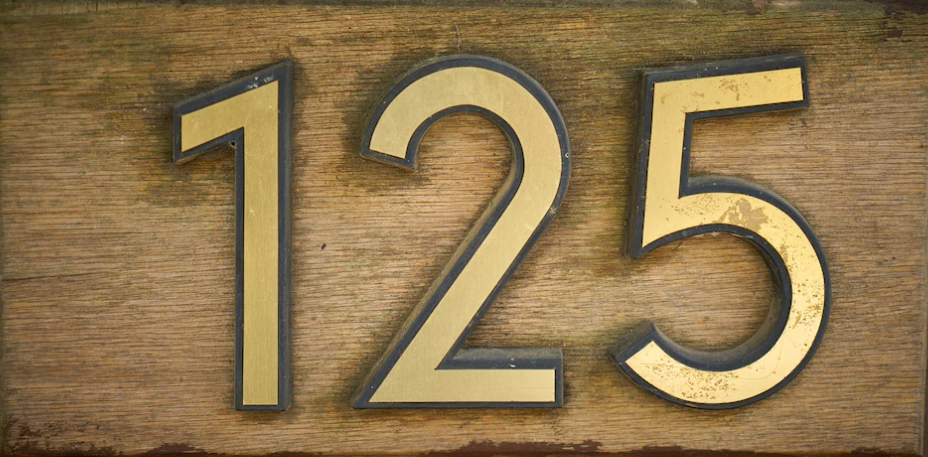
\includegraphics[width=0.37503in,height=0.40003in]{media/image9.png}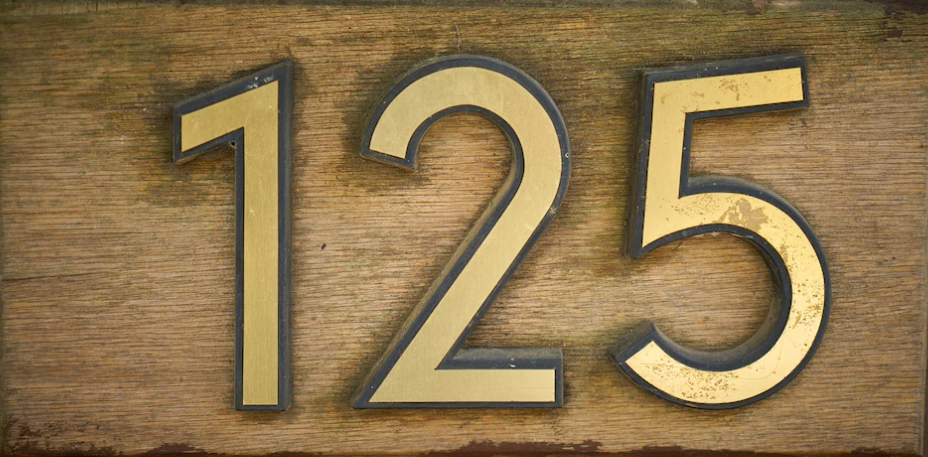
\includegraphics[width=0.37503in,height=0.40003in]{media/image9.png}
\includegraphics[width=0.38337in,height=0.31669in]{media/image10.png}
\includegraphics[width=0.38337in,height=0.31669in]{media/image10.png}
\includegraphics[width=0.38337in,height=0.31669in]{media/image10.png}
\includegraphics[width=0.31669in,height=0.41670in]{media/image11.png}
\includegraphics[width=0.31669in,height=0.41670in]{media/image11.png}
\includegraphics[width=0.31669in,height=0.41670in]{media/image11.png}
\includegraphics[width=0.31669in,height=0.41670in]{media/image11.png}
\includegraphics[width=0.31669in,height=0.41670in]{media/image11.png}

\begin{enumerate}
\def\labelenumi{\alph{enumi})}
\item
  1 240
\end{enumerate}


\includegraphics[width=0.39170in,height=0.51671in]{media/image12.png}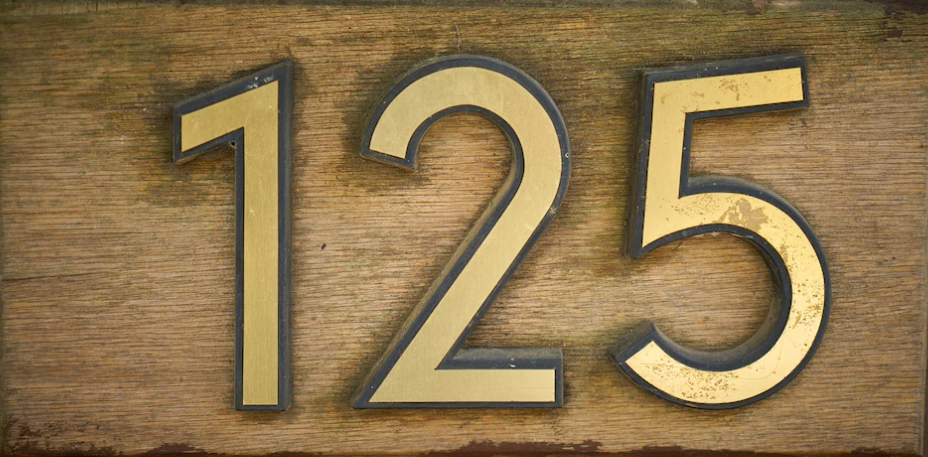
\includegraphics[width=0.37503in,height=0.40003in]{media/image9.png}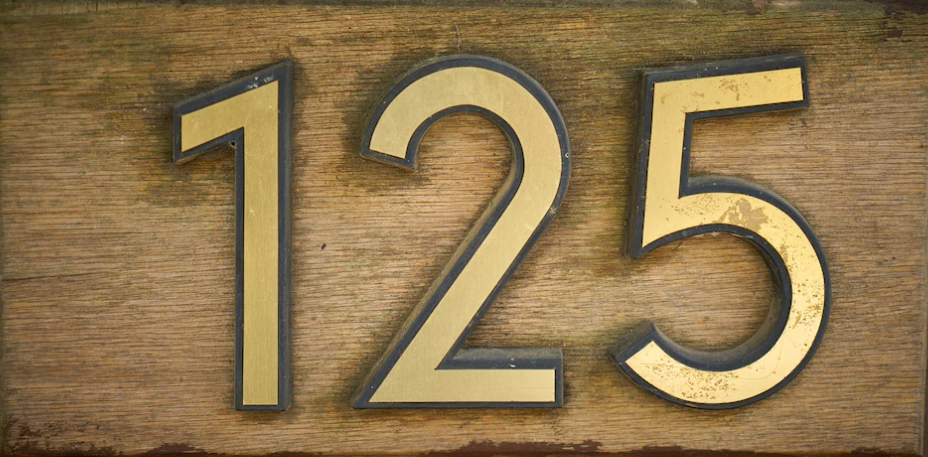
\includegraphics[width=0.37503in,height=0.40003in]{media/image9.png}
\includegraphics[width=0.38337in,height=0.31669in]{media/image10.png}
\includegraphics[width=0.38337in,height=0.31669in]{media/image10.png}
\includegraphics[width=0.38337in,height=0.31669in]{media/image10.png}
\includegraphics[width=0.38337in,height=0.31669in]{media/image10.png}

\begin{enumerate}
\def\labelenumi{\alph{enumi})}
\item
  12 132
\end{enumerate}

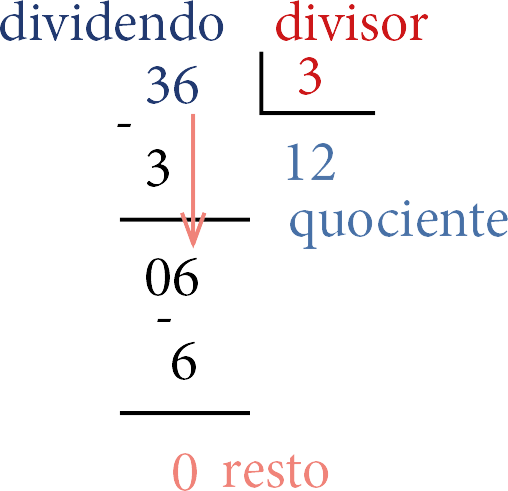
\includegraphics[width=0.33336in,height=0.50004in]{media/image13.png}
\includegraphics[width=0.39170in,height=0.51671in]{media/image12.png}
\includegraphics[width=0.39170in,height=0.51671in]{media/image12.png}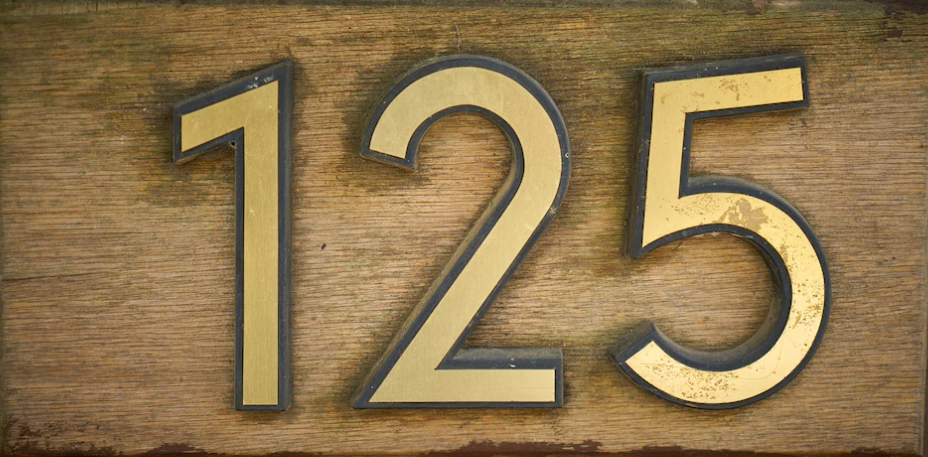
\includegraphics[width=0.37503in,height=0.40003in]{media/image9.png}
\includegraphics[width=0.38337in,height=0.31669in]{media/image10.png}
\includegraphics[width=0.38337in,height=0.31669in]{media/image10.png}
\includegraphics[width=0.38337in,height=0.31669in]{media/image10.png}
\includegraphics[width=0.31669in,height=0.41670in]{media/image11.png}
\includegraphics[width=0.31669in,height=0.41670in]{media/image11.png}

\subsubsection{7.}\label{section-6}

Realize a correspondência entre os retângulos da coluna 1 e os círculos
da segunda coluna, traçando linhas retas.

O maior número com exatamente 5 ordens 147 254

O segundo maior número formado por 4 ordens 464 823

Um número ímpar com 6 ordens 99 999

Um número de 6 ordens com algarismo da unidade de milhar igual a 7 9 998

Os números escritos por extenso devem estar dentro de retângulos com o
fundo preenchido com uma cor e os números da coluna 2 devem estar dentro
de círculos com o fundo preenchido com uma cor

Resposta:

O maior número com exatamente 5 ordens deverá estar ligado a 99 999

O segundo maior número formado por 4 ordens deverá estar ligado a 9 998

Um número ímpar com 6 ordens deverá estar ligado a 464 823

Um número de 6 ordens com algarismo da unidade de milhar igual a 7
deverá estar ligado a 147 254.

Professor explore ao máximo o conceito de par e ímpar e já comece a
introduzir o conceito sequencial dos números naturais, em que após uma
sempre vem um ímpar e que depois de um ímpar sempre vem um par desde que
estejam todos os números naturais escritos.

Além disso, já pode ser introduzido o conceito de sucessor e antecessor
que virá mais a frente dizendo que 9 999 e sucessor de 9 998 e que 9 998
é o antecessor de 9 999.

\subsubsection{8.}\label{section-7}

Represente os números a seguir utilizando os símbolos Maias.

\begin{enumerate}
\def\labelenumi{\alph{enumi})}
\item
  11
\end{enumerate}

Deixar uma linha para resposta

\begin{enumerate}
\def\labelenumi{\alph{enumi})}
\item
  12
\end{enumerate}

Deixar uma linha para resposta

\begin{enumerate}
\def\labelenumi{\alph{enumi})}
\item
  13
\end{enumerate}

Deixar uma linha para resposta

\begin{enumerate}
\def\labelenumi{\alph{enumi})}
\item
  14
\end{enumerate}

Deixar uma linha para resposta

\begin{enumerate}
\def\labelenumi{\alph{enumi})}
\item
  15
\end{enumerate}

Deixar uma linha para resposta

\begin{enumerate}
\def\labelenumi{\alph{enumi})}
\item
  16
\end{enumerate}

Deixar uma linha para resposta

\begin{enumerate}
\def\labelenumi{\alph{enumi})}
\item
  17
\end{enumerate}

Deixar uma linha para resposta

\begin{enumerate}
\def\labelenumi{\alph{enumi})}
\item
  18
\end{enumerate}

Deixar uma linha para resposta

\begin{enumerate}
\def\labelenumi{\alph{enumi})}
\item
  19
\end{enumerate}

Deixar uma linha para resposta

Resposta:

\begin{enumerate}
\def\labelenumi{\alph{enumi})}
\item
  11
\end{enumerate}

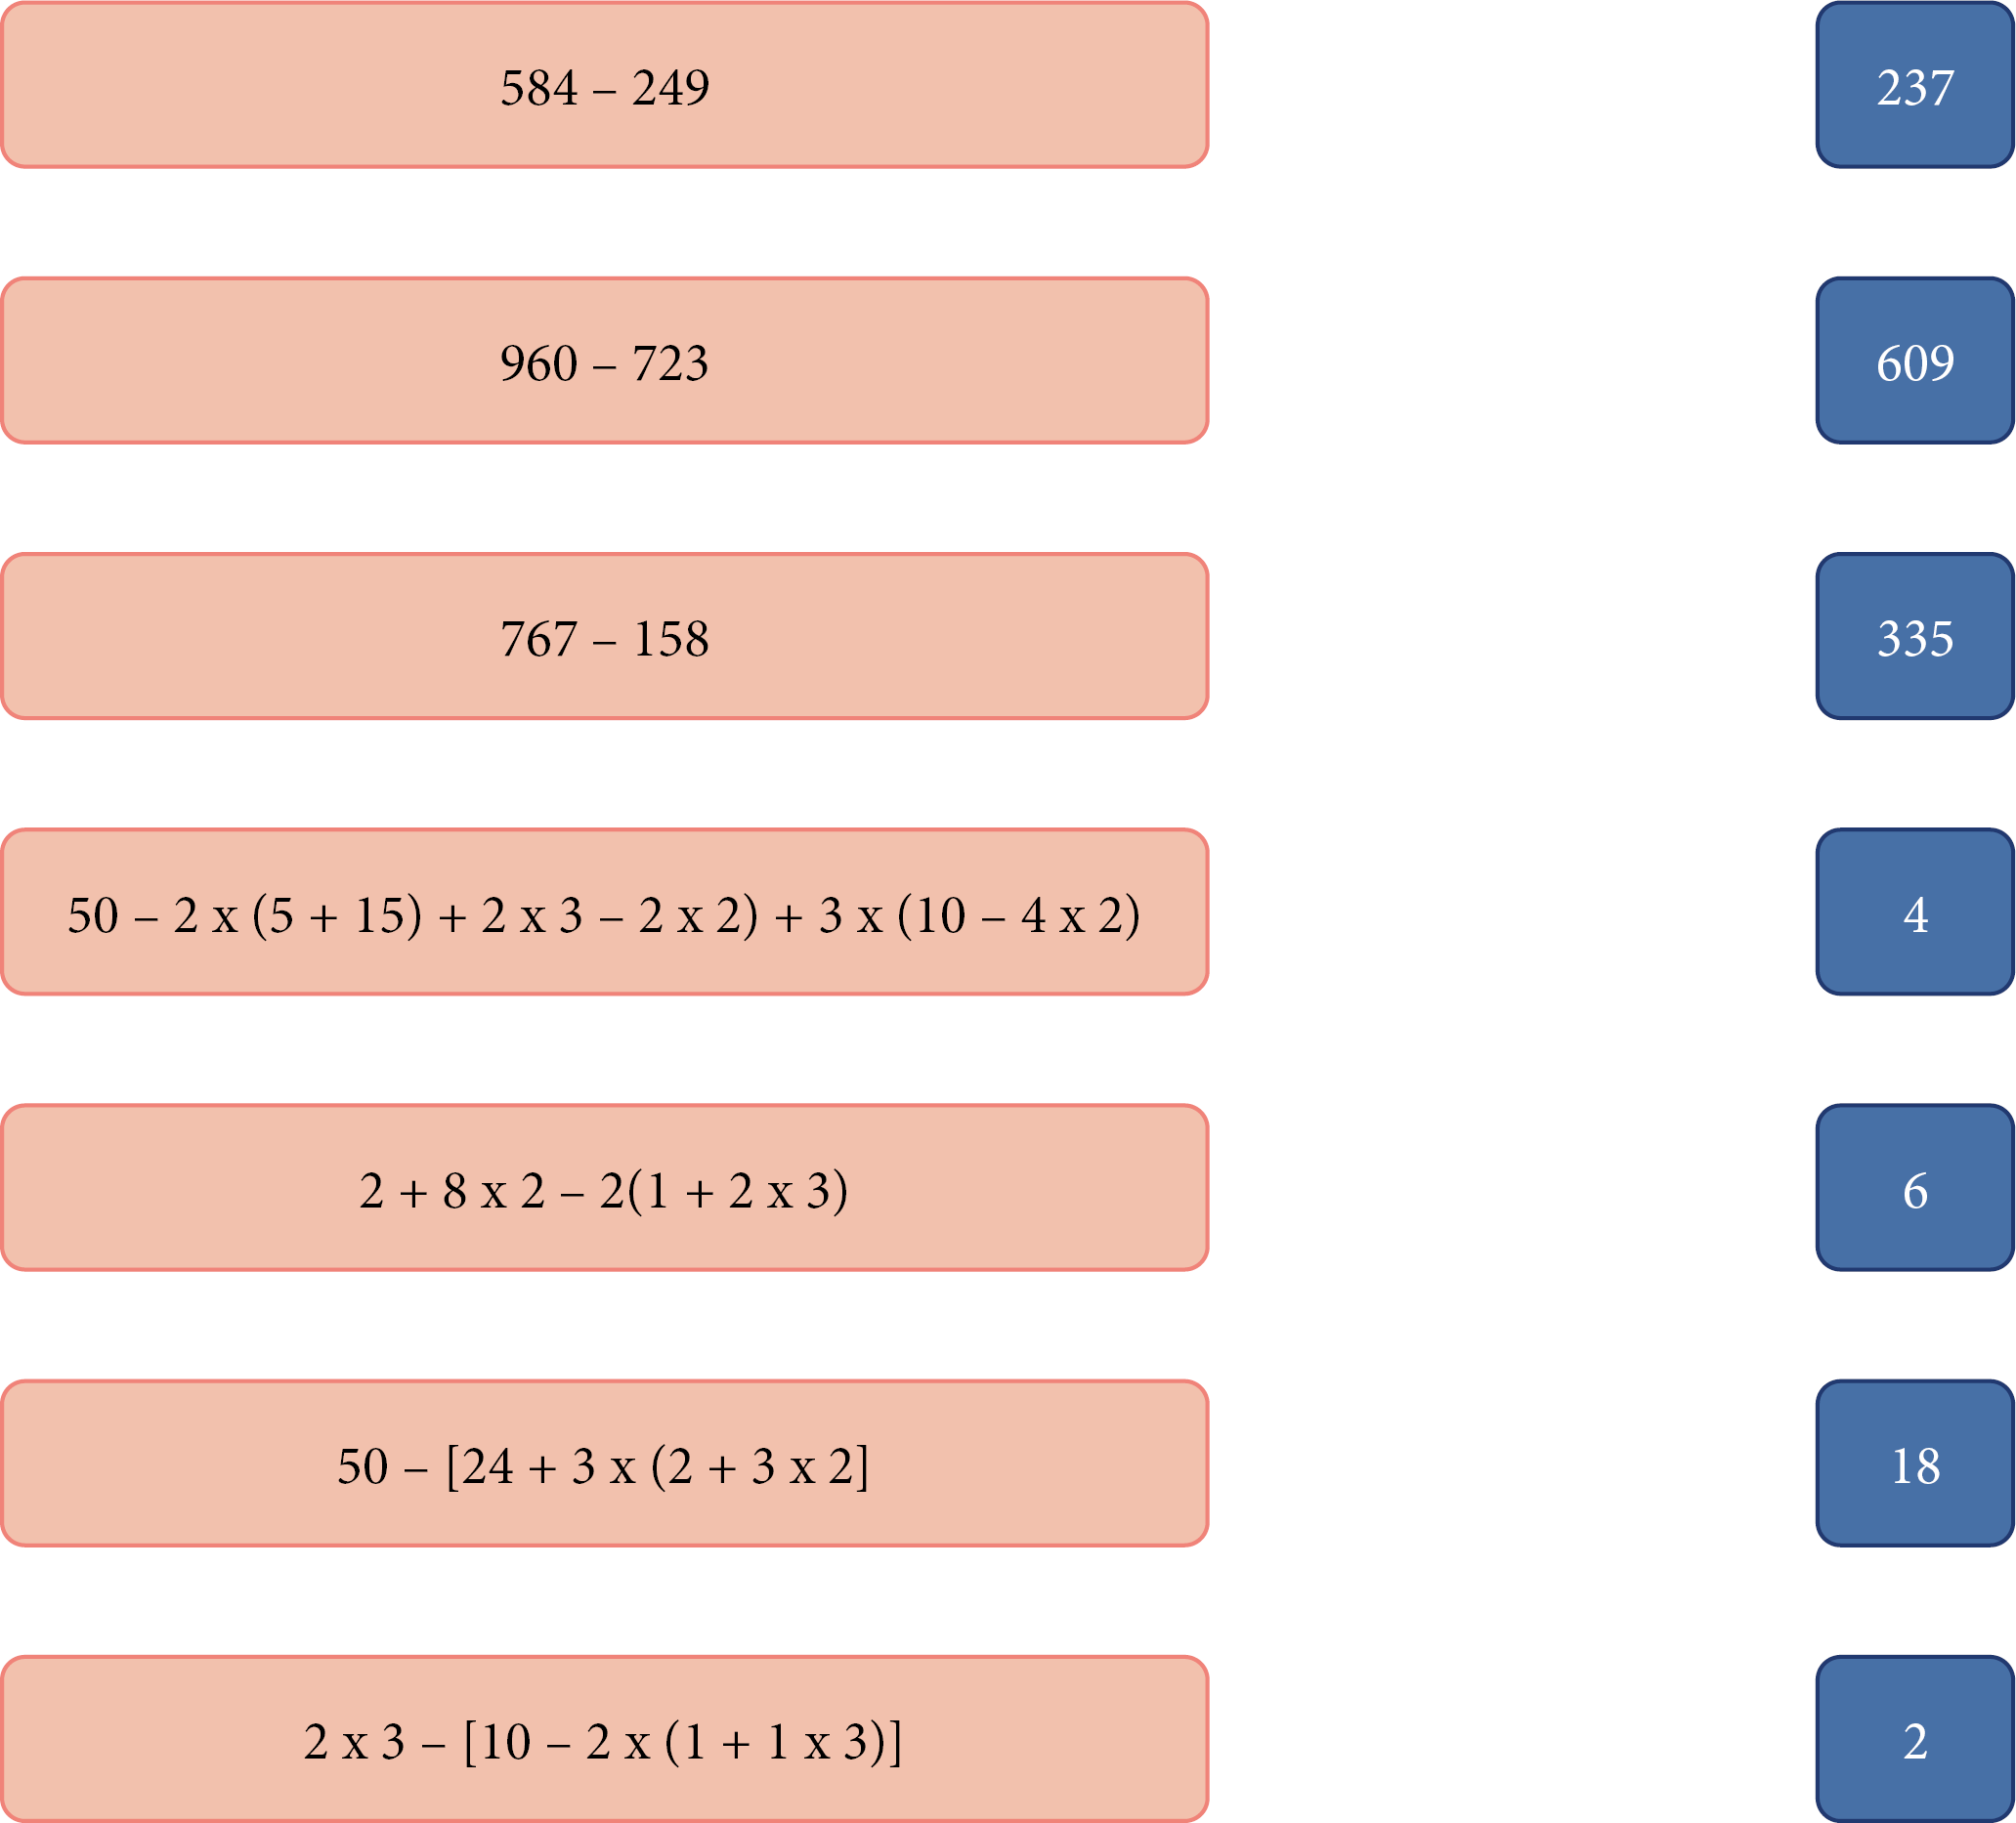
\includegraphics[width=0.50004in,height=0.26669in]{media/image14.png}
\includegraphics[width=0.25836in,height=0.18335in]{media/image15.png}

\begin{enumerate}
\def\labelenumi{\alph{enumi})}
\item
  12
\end{enumerate}

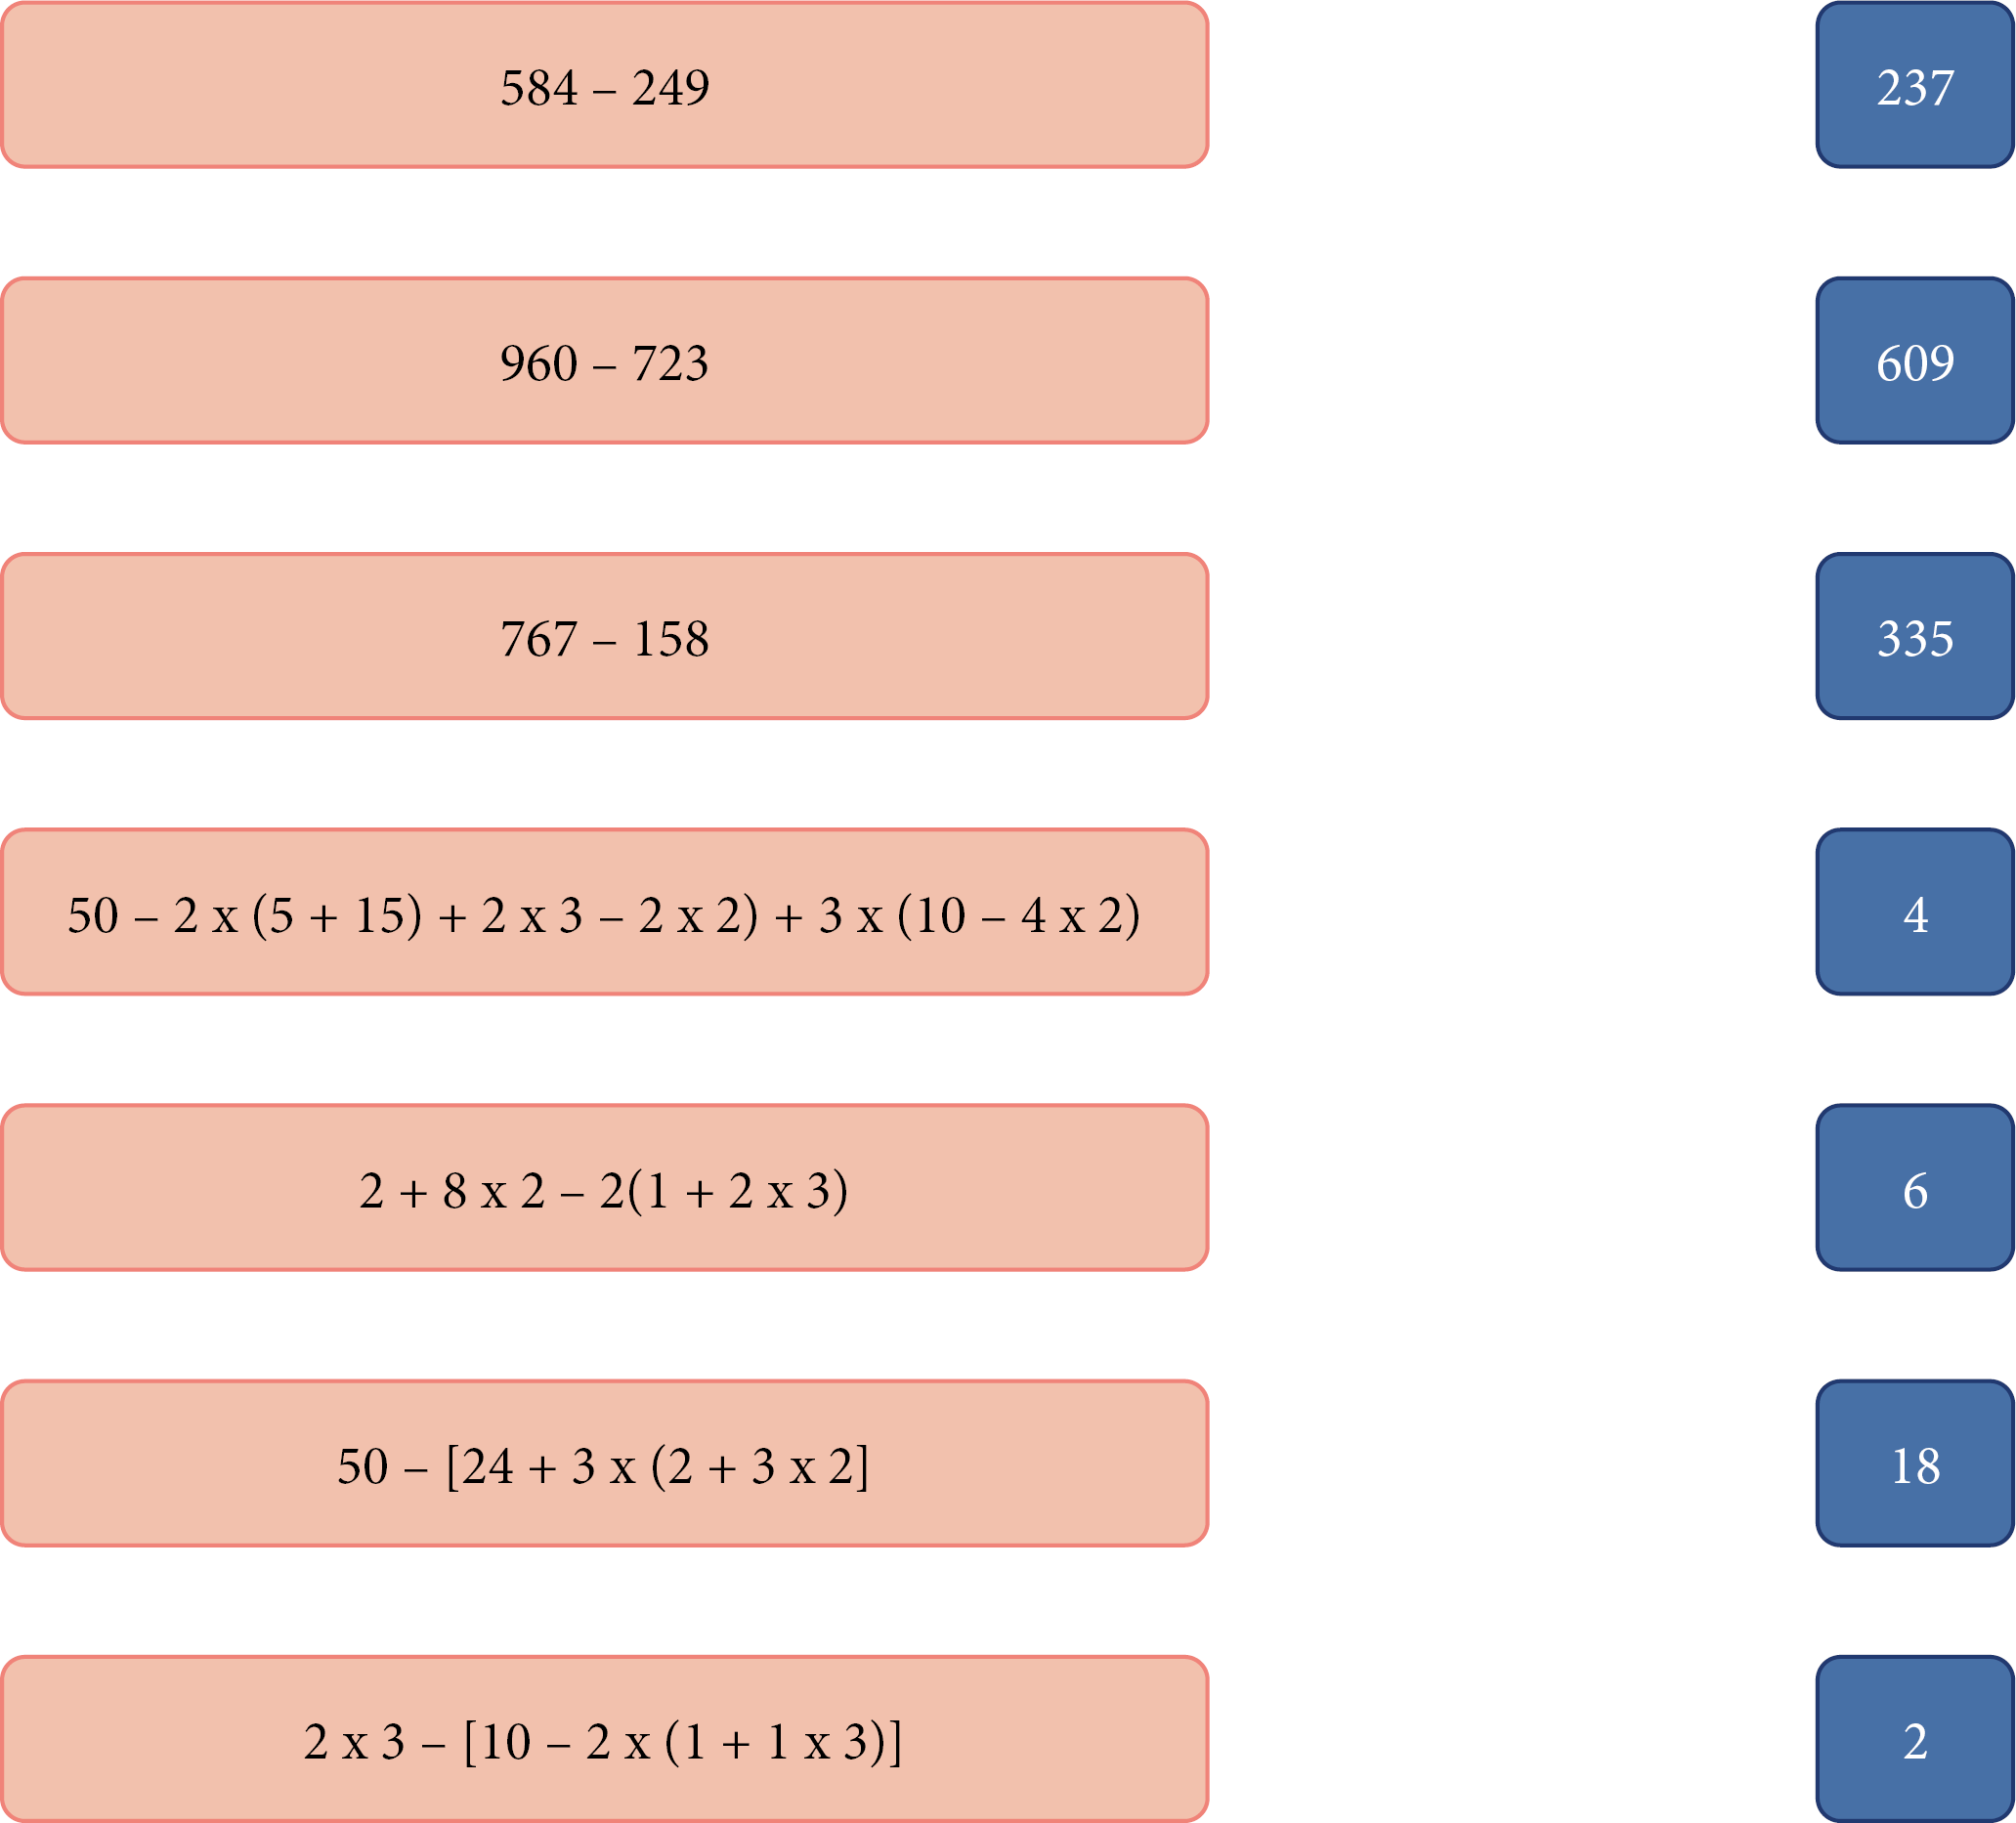
\includegraphics[width=0.50004in,height=0.26669in]{media/image14.png}
\includegraphics[width=0.25836in,height=0.18335in]{media/image15.png}
\includegraphics[width=0.25836in,height=0.18335in]{media/image15.png}

\begin{enumerate}
\def\labelenumi{\alph{enumi})}
\item
  13
\end{enumerate}

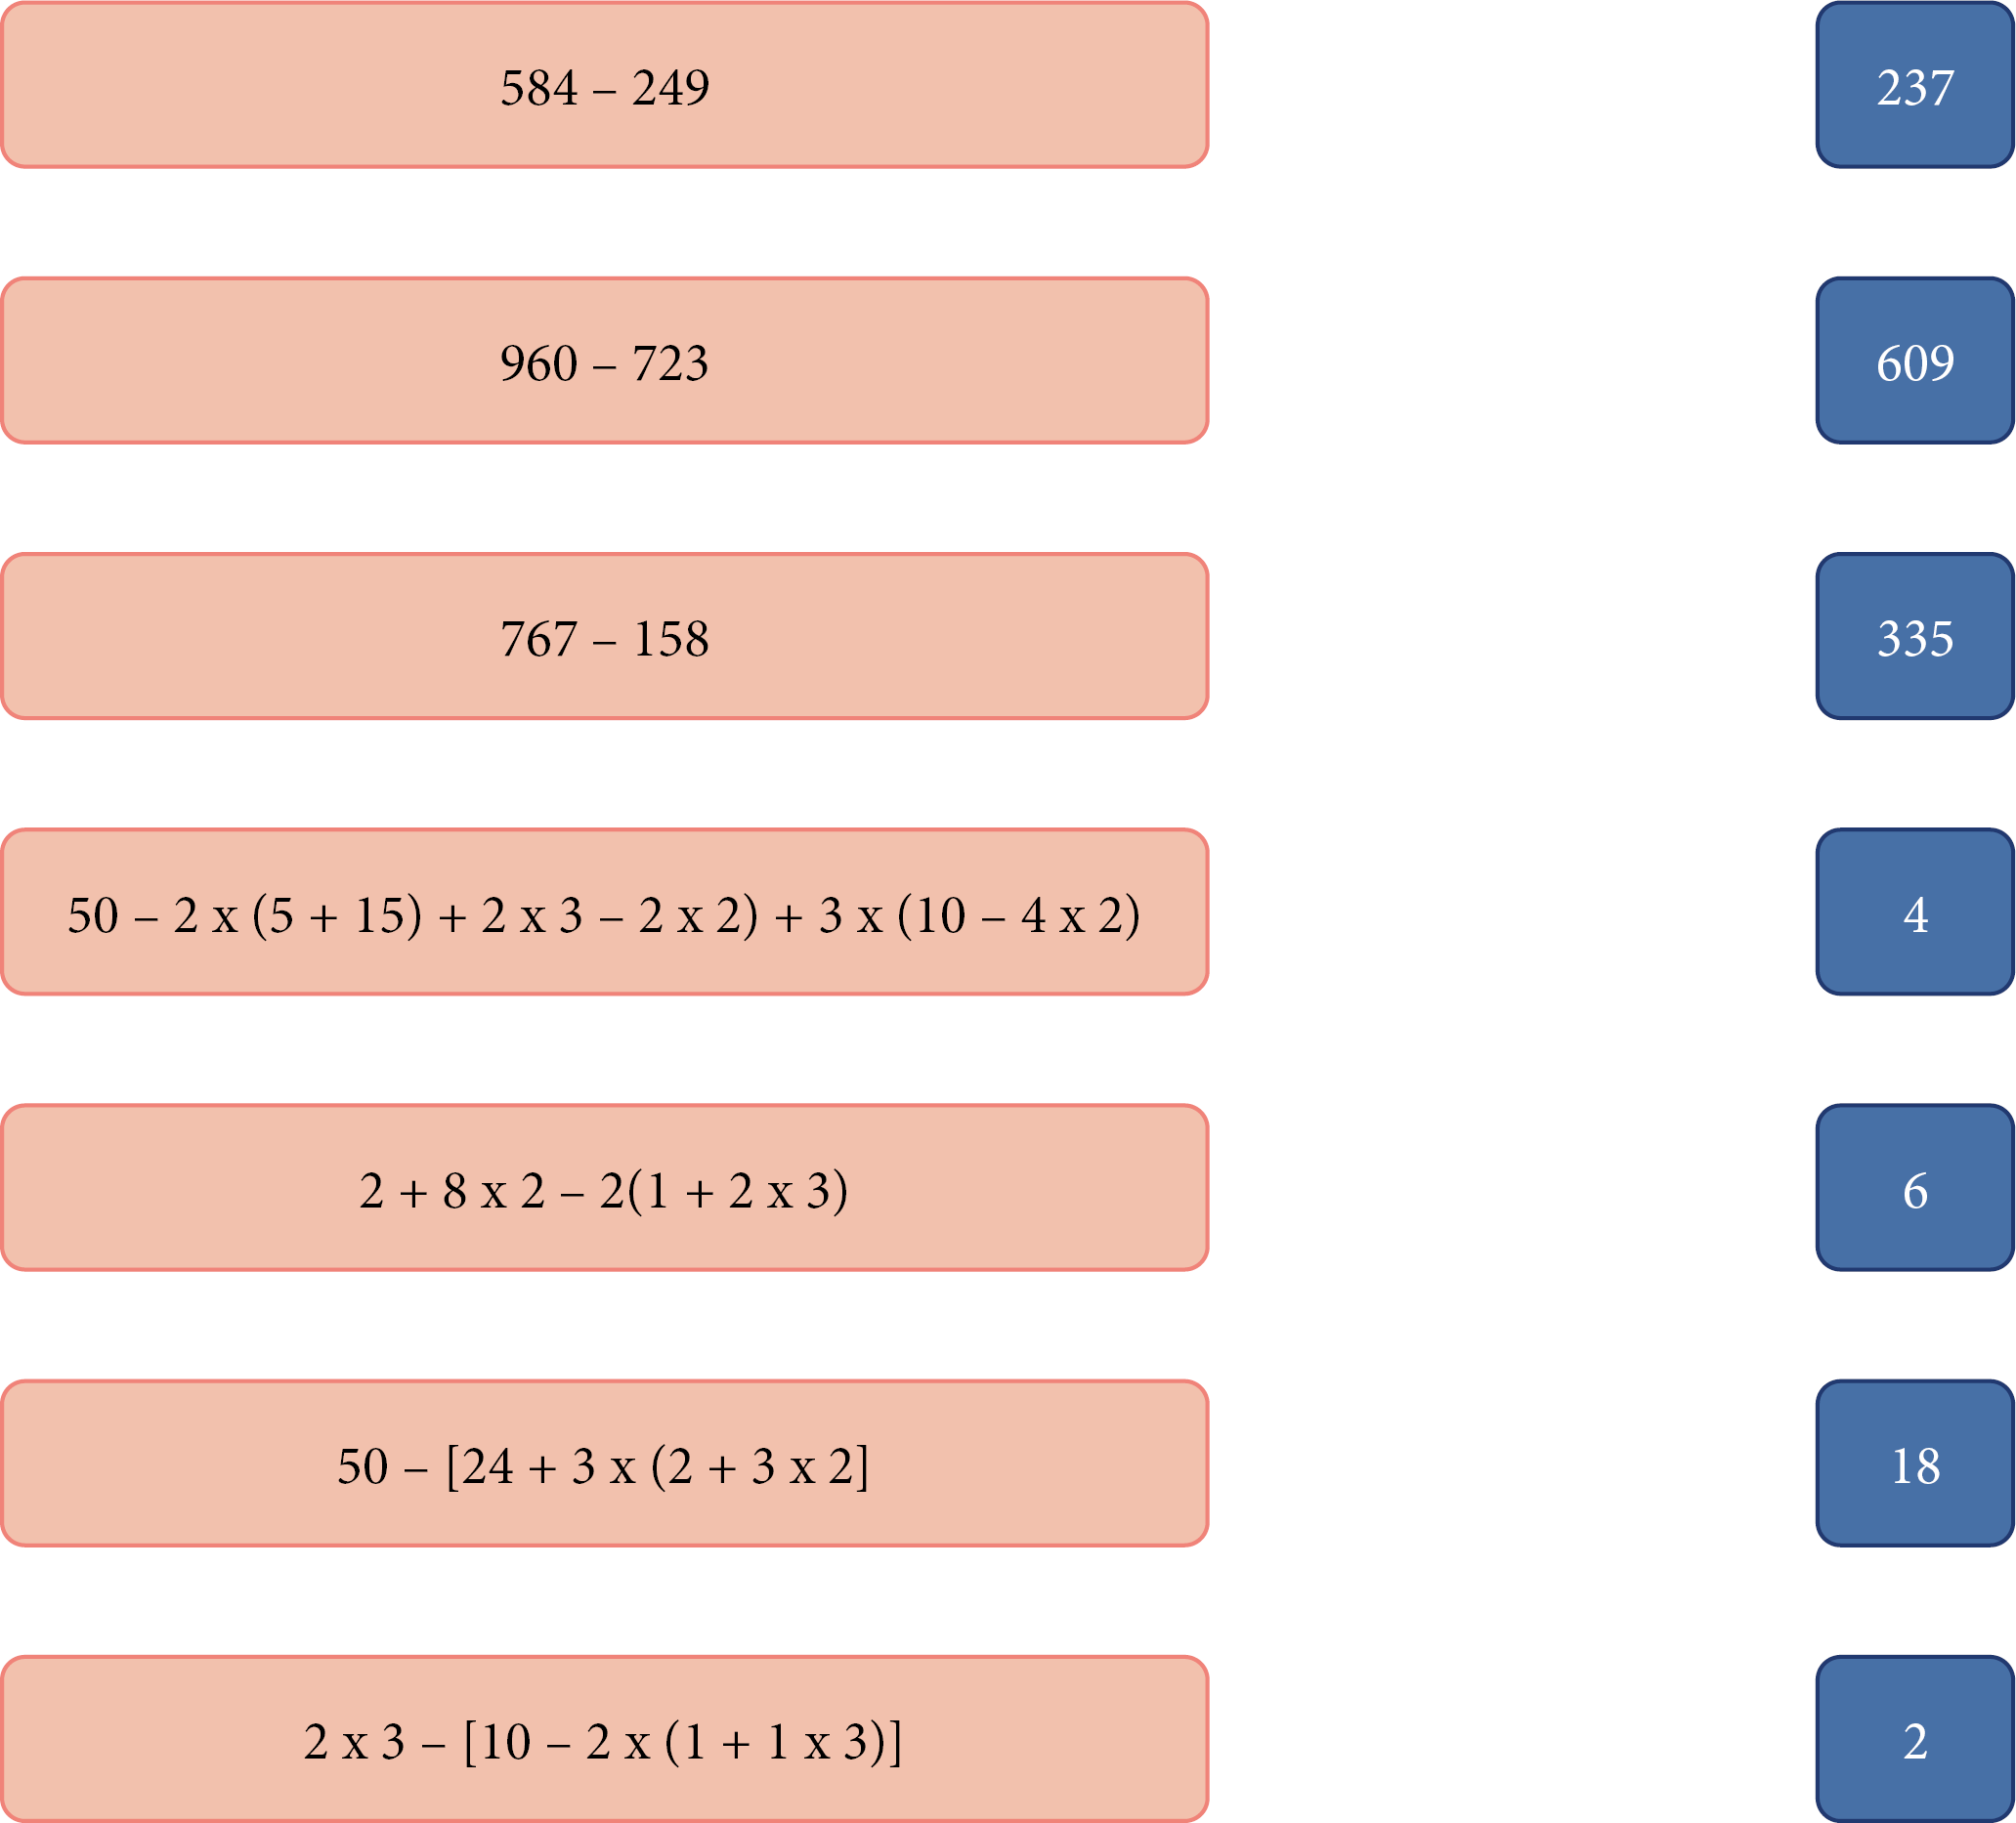
\includegraphics[width=0.50004in,height=0.26669in]{media/image14.png}
\includegraphics[width=0.25836in,height=0.18335in]{media/image15.png}
\includegraphics[width=0.25836in,height=0.18335in]{media/image15.png}
\includegraphics[width=0.25836in,height=0.18335in]{media/image15.png}

\begin{enumerate}
\def\labelenumi{\alph{enumi})}
\item
  14
\end{enumerate}

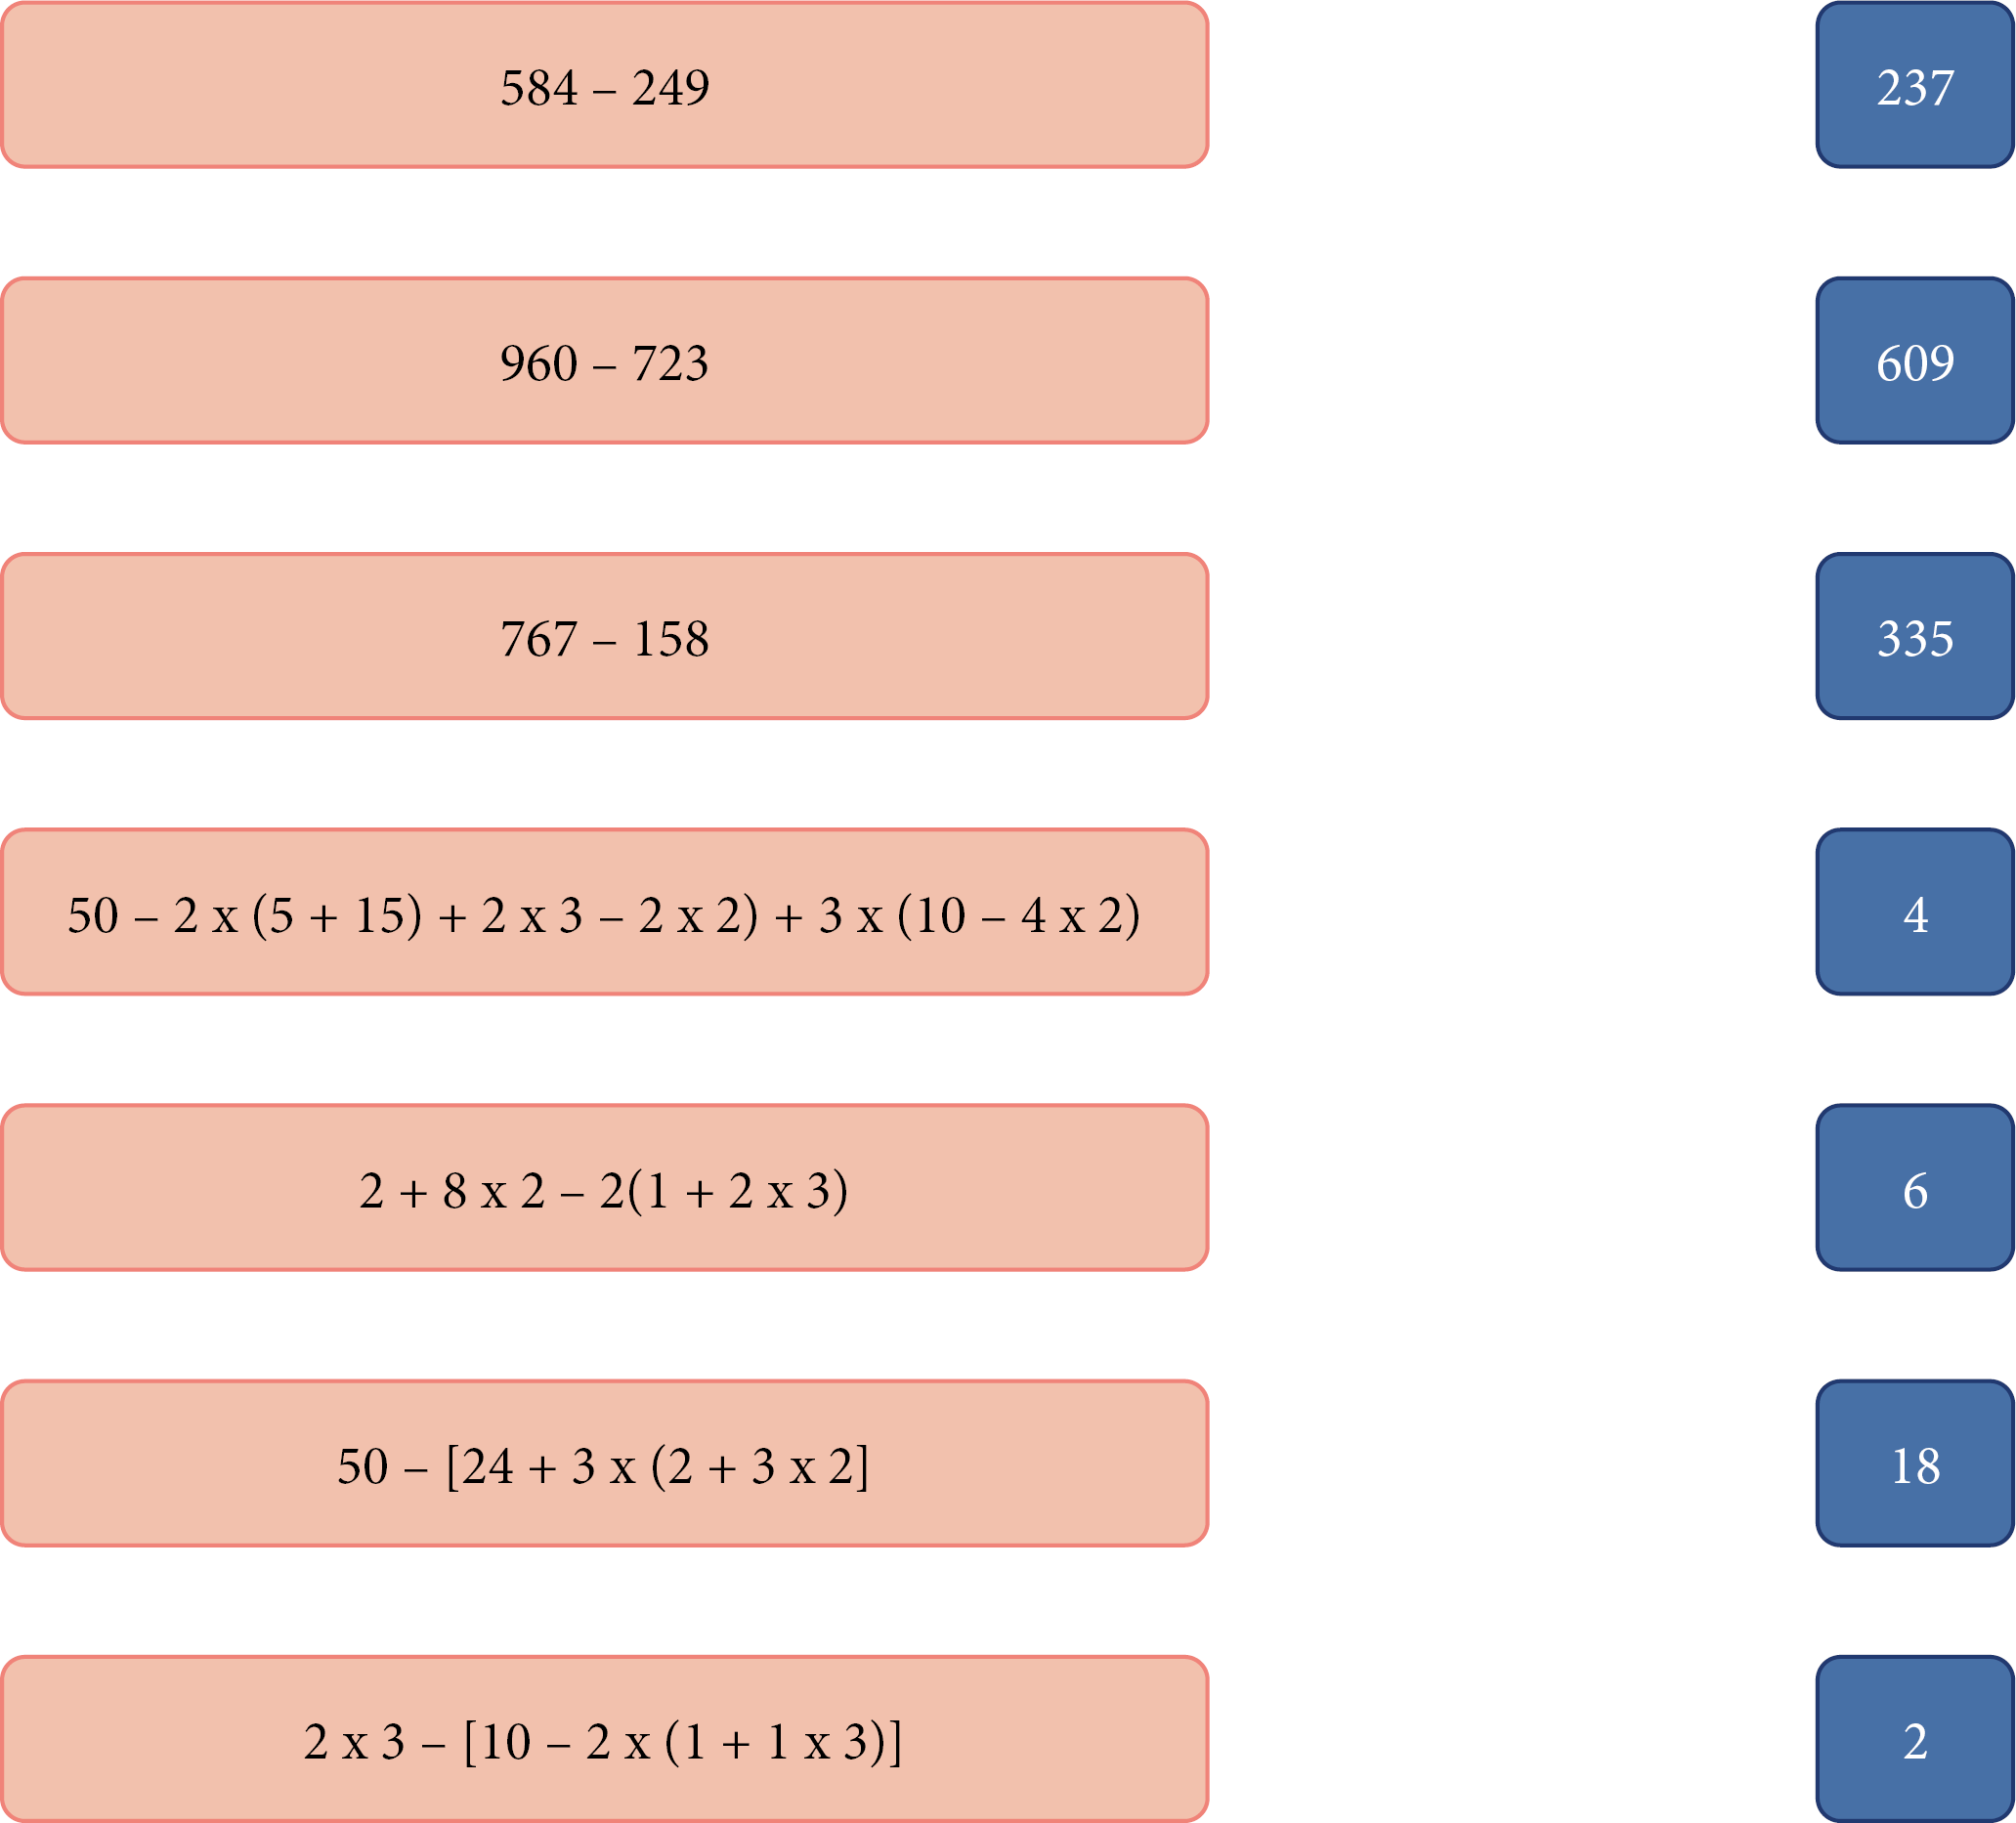
\includegraphics[width=0.50004in,height=0.26669in]{media/image14.png}
\includegraphics[width=0.25836in,height=0.18335in]{media/image15.png}\includegraphics[width=0.25836in,height=0.18335in]{media/image15.png}\includegraphics[width=0.25836in,height=0.18335in]{media/image15.png}\includegraphics[width=0.25836in,height=0.18335in]{media/image15.png}

\begin{enumerate}
\def\labelenumi{\alph{enumi})}
\item
  15
\end{enumerate}

\includegraphics[width=0.50004in,height=0.26669in]{media/image14.png}\includegraphics[width=0.47504in,height=0.18335in]{media/image16.png}

\begin{enumerate}
\def\labelenumi{\alph{enumi})}
\item
  16
\end{enumerate}

\includegraphics[width=0.50004in,height=0.26669in]{media/image14.png}\includegraphics[width=0.48337in,height=0.30836in]{media/image17.png}

\begin{enumerate}
\def\labelenumi{\alph{enumi})}
\item
  17
\end{enumerate}

\includegraphics[width=0.50004in,height=0.26669in]{media/image14.png}\includegraphics[width=0.43337in,height=0.29169in]{media/image18.png}

\begin{enumerate}
\def\labelenumi{\alph{enumi})}
\item
  18
\end{enumerate}

\includegraphics[width=0.50004in,height=0.26669in]{media/image14.png}\includegraphics[width=0.39170in,height=0.26669in]{media/image19.png}

\begin{enumerate}
\def\labelenumi{\alph{enumi})}
\item
  19
\end{enumerate}

\includegraphics[width=0.50004in,height=0.26669in]{media/image14.png}\includegraphics[width=0.43337in,height=0.25836in]{media/image20.png}

\subsubsection{9.}\label{section-8}

Escreva cada um dos números abaixo utilizando o sistema indo-arábico.

\begin{enumerate}
\def\labelenumi{\alph{enumi})}
\item
  Dois mil trezentos e cinco\_\_\_\_\_\_\_\_\_\_\_\_\_
\item
  Quinze mil e quarenta e sete.\_\_\_\_\_\_\_\_\_\_\_\_\_
\item
  Vinte mil e novecentos.\_\_\_\_\_\_\_\_\_\_\_\_\_\_
\item
  Trinta e três mil trezentos e trinta e três.\_\_\_\_\_\_\_\_\_\_\_\_\_
\item
  Cinquenta mil e cinco\_\_\_\_\_\_\_\_\_\_\_\_\_\_\_\_\_\_\_\_
\end{enumerate}

Resposta:

\begin{enumerate}
\def\labelenumi{\alph{enumi})}
\item
  2 305
\item
  15 047
\item
  20 900
\item
  33 333
\item
  50 005
\end{enumerate}

\subsubsection{10.}\label{section-9}

A bolas representadas abaixo fazem parte de um jogo conhecido como
bilhar ou sinuca.

\includegraphics[width=1.40833in,height=1.33406in]{media/image21.png}

\url{https://img.freepik.com/vetores-premium/bola-de-bilhar-azul-com-numero-2-snooker-ou-bola-de-loteria-em-fundo-branco-ilustracao_390775-925.jpg?w=740}

\includegraphics[width=1.66667in,height=1.61877in]{media/image22.png}

\url{https://img.freepik.com/vetores-premium/bilhar_672017-1383.jpg?w=740}

\includegraphics[width=1.68333in,height=1.36449in]{media/image23.png}

\url{https://img.freepik.com/psd-premium/ilustracao-3d-da-bola-de-bilhar-oito_446709-517.jpg?w=740}

\includegraphics[width=1.61667in,height=1.60236in]{media/image24.png}

\url{https://img.freepik.com/psd-premium/bola-de-bilhar-3d-numero-9_592419-130.jpg?w=740}

Colocar as bolinhas na mesma linha

Observando os números representados em cada bola e responda:

\begin{enumerate}
\def\labelenumi{\alph{enumi})}
\item
  Qual o menor número?
\item
  Qual o menor com exatamente 4 ordens podemos formar número?
\item
  Qual o maior número par que podemos formar?
\end{enumerate}

Resposta:

\begin{enumerate}
\def\labelenumi{\alph{enumi})}
\item
  2 (dois)
\item
  2 789 (dois mil setecentos e oitenta e nove)
\item
  9 872 (nove mil oitocentos e setenta e dois)
\end{enumerate}

Explore mais exemplos com os alunos para estimular a formação de número
e a criatividade de cada um deles.

\subsection{Treino}\label{treino}

\subsubsection{1.}\label{section-10}

Amanda estava brincando no escritório de seu pai quando encontrou um
pedaço de papel.

\includegraphics[width=3.30833in,height=2.17391in]{media/image25.png}

\url{https://img.freepik.com/vetores-gratis/vetor-de-fundo-de-design-de-pedaco-de-papel-rasgado_1055-13108.jpg?w=900\&t=st=1677434705~exp=1677435305~hmac=787f679840c02b57af4cb87ef851030bb83880366602641e4486462d6d3553f8}

No pedaço de papel colocar bem grande a frase abaixo escrita:

Faturamento semestral: 650 734 reais

Lembrando das aulas de matemática ela resolveu decompor o número escrito
no papel. Qual a decomposição correta que Amanda deverá fazer desse
número?

\begin{enumerate}
\def\labelenumi{\alph{enumi})}
\item
  600 000 + 50 000 + 700 + 30 + 4
\item
  600 000 + 5 000 + 70 + 3 + 4
\item
  600 000 + 500 + 700 + 30 + 4
\item
  60 000 + 50 000 + 70 + 300 + 4
\end{enumerate}

Resposta: A

600 000 + 50 000 + 700 + 30 + 4

\subsubsection{2.}\label{section-11}

Vitor escreveu o seguinte número utilizando os algarismos romanos:

XIX

Esse número no sistema indo-arábico seria o:

\begin{enumerate}
\def\labelenumi{\alph{enumi})}
\item
  9
\item
  19
\item
  21
\item
  11
\end{enumerate}

Resposta: B

Esse número é o 19 (dezenove) no nosso sistema de numeração.

\subsubsection{3.}\label{section-12}

José resolveu comprar uma linda placa com o número de sua casa.

\includegraphics[width=3.02500in,height=1.48973in]{media/image26.png}

\url{https://img.freepik.com/fotos-gratis/numero-125_1122-1156.jpg?w=1060\&t=st=1677434865~exp=1677435465~hmac=526ac25f92ac28e692177f84842345ca95b5e246e04ca35259750459c4f3e954}

Porém na hora de efetuar a compra não percebeu que o número estava
errado já que o primeiro e o último algarismos estão nas posições
trocadas. Qual o valor relativo do último algarismo no lugar que ele se
encontra na placa errada e qual deveria ser seu valor relativo no número
correto da casa de José?

\begin{enumerate}
\def\labelenumi{\alph{enumi})}
\item
  Como está: 5 Como deveria ser: 50
\item
  Como está: 50 Como deveria ser: 500
\item
  Como está: 5 Como deveria ser: 500
\item
  Como está: 50 Como deveria ser: 5
\end{enumerate}

Resposta: C

Como o número apresentado no enunciado está com o primeiro e o último
algarismos trocados, conclui-se que o número correto seria 524. Na placa
o último algarismo é o 5 e tem valor relativo de 5 unidades, mas no
número correto ele estaria na centena comum, possuindo, então, um valor
relativo de 500 (quinhentos).

\section{Módulo 2}\label{muxf3dulo-2}

Habilidade BNCC: EF04MA07

Habilidades Saeb:

- Calcular o resultado de adições ou subtrações envolvendo números
naturais de até 6 ordens.

- Calcular o resultado de multiplicações ou divisões envolvendo números
naturais de até 6 ordens.

- Associar o quociente de uma divisão com resto zero de um número
natural de até 6 ordens por 2, 3, 4, 5 e 10 às ideias de metade, terça,
quarta, quinta e décima parte.

- Resolver problemas de adição ou de subtração, envolvendo números
naturais de até 6 ordens, com os significados de juntar, acrescentar,
separar, retirar, comparar ou completar.

- Resolver problemas de multiplicação ou de divisão, envolvendo números
naturais de até 6ordens, com os significados de formação de grupos
iguais (incluindo repartição equitativa e medida), proporcionalidade ou
disposição retangular.

\subsection{Conteúdo}\label{conteuxfado-1}

\protect\hypertarget{_Hlk128407586}{}{}Professores talvez esse seja um
dos módulos mais importantes por se tratar das quatro operações básicas.
Relembre com os alunos cada detalhe e algoritmos da adição, subtração,
multiplicação e divisão dando uma ênfase enorme na divisão que
geralmente é o maior problema enfrentado pelos alunos.

Adição:

Fazer a imagem abaixo segundo os padrões do projeto.

\includegraphics[width=2.26282in,height=1.19473in]{media/image27.png}

Subtração:

Fazer a imagem abaixo segundo os padrões do projeto.

\includegraphics[width=2.55128in,height=1.04961in]{media/image28.png}

Outro exemplo com descrição do que deve ser feito

\includegraphics[width=3.89200in,height=2.81691in]{media/image29.png}

Multiplicação:

Fazer a imagem abaixo segundo os padrões do projeto.

\includegraphics[width=1.92308in,height=1.09649in]{media/image30.png}

Divisão:

Fazer a imagem abaixo segundo os padrões do projeto.

\includegraphics[width=2.26923in,height=1.66995in]{media/image31.png}

\subsection{Atividades}\label{atividades-1}

\subsubsection{1.}\label{section-13}

Ligue cada operação que está na coluna 1 com o seu resultado correto na
coluna 2.

584 -- 249 237

960 -- 723 609

767 -- 158 335

50 -- 2 x (5 + 15) + 2 x 3 -- 2 x 2) + 3 x (10 -- 4 x 2) 4

2 + 8 x 2 -- 2(1 + 2 x 3) 6

50 -- {[}24 + 3 x (2 + 3 x 2{]} 18

2 x 3 -- {[}10 -- 2 x (1 + 1 x 3){]} 2

Colocar as operações acima e os resultados de ambas as colunas em
retângulos

Deixar um espaço em branco referente a 10 linhas para os alunos
efetuarem os cálculos necessários

Resposta:

Professor explore ao máximo com os alunos o conceito de quais operações
devem ser realizadas primeiro e assim fixo esse conceito da ordem das
operações.

584 -- 249 = 335

960 -- 723 = 237

767 -- 158 = 609

50 -- 2 x (5 + 15) + 2 x (3 -- 2 x 1) + 3 x (10 -- 4 x 2) = 50 -- 40 + 2
+ 6 = 18

2 + 8 x 2 -- 2(1 + 2 x 3) = 2 + 16 -- 14 = 4

50 -- {[}24 + 3 x (2 + 3 x 2{]} = 50 -- 48 = 2

2 x 4 -- {[}10 -- 2 x (1 + 1 x 3){]} = 8 -- 2 = 6

\subsubsection{2.}\label{section-14}

\includegraphics[width=3.00000in,height=2.02528in]{media/image32.png}A
receita de um bolo diz que inicialmente devemos colocar 260 g de farinha
de trigo e misturar com outros ingredientes como ovos, açúcar e leite.
Um seguida, devemos colocar mais 135 g de farinha de trigo para a massa
ficar no ponto ideal. Qual foi a quantidade total de farinha, em quilos,
utilizada nessa receita?

https://img.freepik.com/fotos-premium/chef-cozinheiro-confeiteiro-ou-padeiro-em-t-shirt-branca-toque-chefs-chapeu-cozinhando-na-mesa-isolada-em-fundo-rosa-pastel-em-estudio-aplicacao-de-creme-processo-de-confeccao-de-bolos-mock-up-conceito-de-comida-de-espaco-de-copia\_365776-27137.jpg?w=1060

Deixar espaço em branco de 3 linhas para a resolução

Resposta:

260 + 135 = 395 g = 0,395 kg

\subsubsection{3.}\label{section-15}

O estado de São Paulo tem muitas cidades sendo que muitas delas com
centenas de milhares de habitantes. A tabela mostra a população estimada
de algumas cidades paulistas.

\begin{longtable}[]{@{}ll@{}}
\toprule
Município & População estimada\tabularnewline
\midrule
\endhead
São Paulo & 12 396 372\tabularnewline
Campinas & 1 223 237\tabularnewline
Ribeirão Preto & 720 116\tabularnewline
Franca & 358 539\tabularnewline
São Carlos & 256 915\tabularnewline
\bottomrule
\end{longtable}

Dados IBGE.

Sem considerar a cidade de São Paulo, a soma da população estimada das
outras quatro cidades é maior ou menor do que a quantidade de habitantes
da cidade de São Paulo? Justifique com os cálculos.

Deixar espaço de 5 linhas para cálculos

Resposta:

1 223 237 + 720 116 + 358 539 + 256 915 = 2 558 807

Portanto a soma das populações estimadas dos municípios apresentados na
tabela, exceto São Paulo, é menor que a população da cidade de São
Paulo.

\subsubsection{4.}\label{section-16}

Faça o que se pede:

\begin{enumerate}
\def\labelenumi{\alph{enumi})}
\item
  Se em uma caixa cabem 1 000 bolinhas de gude de mesmo tamanho, quantas
  caixas precisaremos para guardar 6 536 bolinhas de gude desse mesmo
  tamanho?
\end{enumerate}

Deixar espaço em branco equivalente a 3 linhas para a resolução

\begin{enumerate}
\def\labelenumi{\alph{enumi})}
\item
  E se a caixa couber só 100 bolinhas de gude de mesmo tamanho, quantas
  caixas serão necessárias para armazenar essas 6 536 bolinhas?
\end{enumerate}

Deixar espaço em branco equivalente a 3 linhas para a resolução

\begin{enumerate}
\def\labelenumi{\alph{enumi})}
\item
  E se agora a caixa só pode armazenar 10 botões, quantas caixas dessas
  serão necessárias para armazenar as 6 536 bolinhas de gude?
\end{enumerate}

Deixar espaço em branco equivalente a 3 linhas para a resolução

Resposta:

\begin{enumerate}
\def\labelenumi{\alph{enumi})}
\item
  6 536/1 000 = 6 e resto 536. Portanto precisaremos de 6 caixas
  completas e mais uma caixa com 536 bolinhas. Total 7 caixas.
\item
  6 536/ 100 = 65 e resto 36. Portanto seguindo o mesmo raciocínio do
  item a, precisaremos de 66 caixas, sendo 65 cheias e uma com as 36
  restantes.
\item
  6 536 / 10 = 653 e resto 6. Com isso, precisaremos de 654 caixas,
  sendo 653 completas e uma com 6 bolinhas de gude.
\end{enumerate}

\subsubsection{5.}\label{section-17}

Complete os quadros abaixo seguindo o raciocínio determinado em cada
item.

\begin{enumerate}
\def\labelenumi{\alph{enumi})}
\item
  Preencha a coluna da tabuada do quatro levando em consideração a
  tabuada do 2 que está preenchida.
\end{enumerate}

\includegraphics[width=3.55833in,height=3.10173in]{media/image33.png}

\begin{enumerate}
\def\labelenumi{\alph{enumi})}
\item
  Preencha a coluna da tabuada do 5 levando em consideração as tabuadas
  do 2 e do 3 que estão preenchidas no quadro.
\end{enumerate}

\includegraphics[width=2.96667in,height=2.58563in]{media/image34.png}

\begin{enumerate}
\def\labelenumi{\alph{enumi})}
\item
  Agora que você já preencheu a coluna do 4, preencha a coluna da
  tabuada do 8 levando em consideração a tabuada do 4.
\end{enumerate}

\includegraphics[width=2.98333in,height=2.55714in]{media/image35.png}

Resposta:

\begin{enumerate}
\def\labelenumi{\alph{enumi})}
\item
\end{enumerate}

\begin{quote}
Colocar na coluna do 4 os seguintes números respectivamente e na
resposta colocar a tabela preenchida.

4; 8; 12; 16; 20; 24; 28; 32; 36

\includegraphics[width=3.55833in,height=3.10173in]{media/image33.png}

Professor explore com os alunos o fato de que conhecendo a tabuada do 2
conseguimos os valores da tabuada do 4 apenas multiplicando os valores
da tabuada do 2 por 2.
\end{quote}

\begin{enumerate}
\def\labelenumi{\alph{enumi})}
\item
\end{enumerate}

\begin{quote}
Colocar na coluna do 5 os seguintes números respectivamente e na
resposta colocar a tabela preenchida.

5; 10; 15; 20; 25; 30; 35; 40; 45

Professor explore com os alunos o fato de que conhecendo as tabuadas do
2 e do 3, conseguimos os valores da tabuada do 5 apenas somando os
valores da tabuada do 2 e da tabuada do 3.
\end{quote}

\includegraphics[width=2.96667in,height=2.58563in]{media/image34.png}

\begin{enumerate}
\def\labelenumi{\alph{enumi})}
\item
\end{enumerate}

\begin{quote}
Colocar na coluna do 8 os seguintes números respectivamente e na
resposta colocar a tabela preenchida.

8; 16; 24; 32; 40; 48; 56; 64; 72

Colocar na coluna do 4 os seguintes números respectivamente e na
resposta colocar a tabela preenchida.

4; 8; 12; 16; 20; 24; 28; 32; 36
\end{quote}

\includegraphics[width=2.98333in,height=2.55714in]{media/image35.png}

\begin{quote}
Professor explore com os alunos o fato de que conhecendo a tabuada do 4
conseguimos os valores da tabuada do 8 apenas multiplicando os valores
da tabuada do 4 por 2.
\end{quote}

\subsubsection{6.}\label{section-18}

O pai de Marcela trabalha em uma transportadora e, em um determinado
dia, seu caminhão foi carregado com 64 engradados de refrigerantes.
Sabendo-se que em cada engradado temos 12 garrafas de refrigerantes e
que em cada garrafa têm-se 2 litros de refrigerante, quantos litros de
refrigerantes o pai de Marcela tinha em seu caminhão?

Deixar espaço em branco equivalente a 3 linhas para a resolução

Resposta:

64 x 12 x 2 = 1 536 litros de refrigerantes

\subsubsection{7.}\label{section-19}

\includegraphics[width=3.00278in,height=1.75833in]{media/image36.png}João
possui uma distribuidora de ovos e acabou de receber 14 caixas com 310
ovos cada uma. Para que João venda essa mercadoria, ele faz embalagens
com 12 ovos cada uma. Quantas embalagens João conseguirá fazer para
colocar à venda utilizando os ovos que acabou de receber em sua loja?
Terá alguma sobra de ovos que não completaram uma embalagem?

https://img.freepik.com/fotos-gratis/ovos-na-superficie-rosa\_58702-1950.jpg?w=1060\&t=st=1677435684\textasciitilde{}exp=1677436284\textasciitilde{}hmac=6c6204dcded4c4d80a06169fee49d53df4b2636105a2c7b3dbe5365007ceae9a

Deixar espaço em branco equivalente a 3 linhas para os cálculos.

Resposta:

(14 x 310):12 = 361 embalagens com 12 ovos cada uma e uma sobra de 8
ovos.

Professor sempre escreva a expressão formada pela interpretação do
enunciado, pois assim irão aprendendo a transformar textos em linguagem
matemática.

\subsubsection{8.}\label{section-20}

O livro que Gabriel está lendo possui 12 capítulos com 22 páginas cada
um. Se ele ler 10 páginas por dia, em quantos dias ele terminará de ler
o livro?

Deixar espaço em branco equivalente a 3 linhas para a resolução

Resposta:

Número de páginas: 12 x 22 = 264

Número de dias: 264/10 = 26 dias lendo 10 páginas por dia e um dia lendo
4 páginas. Portanto terminará o livro em 27 dias.

\subsubsection{9.}\label{section-21}

O pai de Pedro propôs um grande desafio para ele. O desafio consiste em
o pai fornecer uma conta com um número escondido e o filho deveria
descobrir qual número está escondido. Ajude Pedro com esse desafio e
encontre o número que está escondido pelo quadrado.

\includegraphics[width=1.85000in,height=1.43762in]{media/image37.png}

Trocar estrela por um quadrado e colocar a conta acima como se estivesse
em uma folha de caderno.

Resposta:

Realizando a conta de subtração percebesse facilmente que o número
escondido pelo quadrado é o algarismo 1.

\subsubsection{10.}\label{section-22}

Na fazendo do Avô de Vinícius há 104 galinhas, 62 porcos, 6 cavalos e 72
bois. Se na fazendo de seu vizinho o número de animais é o triplo do que
tem na fazenda de seu avô, quantos animais estão presentes na fazenda do
vizinho?

Deixar espaço em branco equivalente a 3 linhas para a resolução

Resposta:

Número de animais na fazenda do avô: 104 + 62 + 6 + 72 = 244

Número de animais na fazenda do vizinho: 3 x 244 = 732 animais.

\subsection{Treino}\label{treino-1}

\subsubsection{1.}\label{section-23}

Verificando algumas atividades realizadas na escola no ano anterior
Gustavo se deparou com a seguinte conta em que um dos números estava
coberto por um retângulo.

\includegraphics[width=5.39213in,height=1.80849in]{media/image38.png}

Fazer uma ilustração nos moldes da acima e nela, trocar o número 178
pelo número 105

Gustavo ficou curioso e resolveu refazer a atividade para descobrir o
número que faltava e, após alguns minutos conseguiu descobrir. Qual o
número que Gabriel encontrou?

\begin{enumerate}
\def\labelenumi{\alph{enumi})}
\item
  128
\item
  312
\item
  158
\item
  256
\end{enumerate}

Resposta: B

417 -- 105 = 312

\subsubsection{2.}\label{section-24}

Isac estava conferindo o estoque de mercadorias de sua loja e percebeu
que inicialmente ele tinha 200 peças, depois vendeu 2 caixas com peças
para Carlos.

Em cada uma das caixas havia um pacote com 5 unidades de peças e dois
pacotes com 7 peças.

Para saber a quantidade de peças que restavam no estoque Isac fez a
seguinte anotação:

200 -- 2 x (1 x 5 + 2 x 7)

O resultado dessa expressão era exatamente igual a quantidade de peças
que restavam em seu estoque após a venda para Carlos. Qual é a
quantidade de peças que Isac possui agora em seu estoque?

\begin{enumerate}
\def\labelenumi{\alph{enumi})}
\item
  72
\item
  94
\item
  126
\item
  162
\end{enumerate}

Resposta: D

200 -- 2 x (1 x 5 + 2 x 7) = 200 -- 38 = 162 peças.

\subsubsection{3.}\label{section-25}

Um grande circo chegou a cidade em que Rafael mora e logo uma fila
enorme se formou com pessoas querendo assistir ao espetáculo. Os
ingressos começaram a ser vendido e as pessoas começaram a entrar no
recinto do circo. Em certo instante sabia-se que 540 pessoas já tinham
entrado e que a capacidade máxima por espetáculo nesse circo era de 1
200 pessoas. Como ainda temos 932 pessoas na fila, quantas pessoas não
conseguirão entrar para assistir a essa seção do circo?

\begin{enumerate}
\def\labelenumi{\alph{enumi})}
\item
  268
\item
  272
\item
  294
\item
  1 440
\end{enumerate}

Resposta: B

1 200 -- 540 = 660

932 -- 660 = 272 pessoas não conseguirão assistir a essa seção.

\section{Módulo 3}\label{muxf3dulo-3}

BNCC: EF04MA11

Habilidades Saeb:

- Inferir ou descrever atributos ou propriedades comuns que os elementos
que constituem uma sequência recursiva de números naturais apresentam.

- Inferir o padrão ou a regularidade de uma sequência de números
naturais ordenados, objetos ou figuras.

- Inferir os elementos ausentes em uma sequência de números naturais
ordenados, objetos ou figuras.

\protect\hypertarget{_Hlk128407765}{}{}Professor durante esse módulo
explore bastante a percepção de seus alunos, deixando realmente durante
a algum tempo que esses tentem descobrir a lógica de cada sentença
assim, possibilitando que consigam descobrir os próximos números de cada
uma. Esse é um conceito essencial para estimular criatividade e
encontrar regras ``escondidas'' entre os números.

\subsection{Conteúdo}\label{conteuxfado-2}

Uma sequência ou sucessão é um conjunto numérico ordenado, na qual,
temos sempre uma lógica para sua formação.

Exemplos:

\begin{itemize}
\item
  A escalação de um time de futebol de salão em ordem alfabética:
\end{itemize}

Alan; Bruno, Fernando, Igor, Tácio.

\begin{itemize}
\item
  Sequência de números naturais pares:
\end{itemize}

(0; 2; 4; 6; 8; 10; 12; ...)

Podemos ainda classificar as sequências quanto ao número de elementos:

\begin{itemize}
\item
  Finitas: Sequências que apresentam um número de termos bem definido,
  ou seja, 10 termos, 20 termos, 8 termos.
\item
  Infinitas: Sequências que apresentam infinitos números de termos como,
  por exemplo, a sequência dos números naturais.
\end{itemize}

Ainda podemos classificar as sequências em:

\begin{itemize}
\item
  Crescente: aquelas em que cada termo sucessor é maior que seu
  antecessor.
\end{itemize}

Exemplo: (5, 10, 15, 20, 25)

\begin{itemize}
\item
  Decrescente: aquelas em que cada termos sucessor sempre é menor do que
  seu antecessor.
\end{itemize}

Exemplo: (9, 7, 5, 3)

\subsection{Atividades}\label{atividades-2}

\subsubsection{1.}\label{section-26}

Observe as sequências dadas e determine, sem fazer desenhos, a
quantidade de bolinhas que a figura 8 de cada sequência terá.

\begin{enumerate}
\def\labelenumi{\alph{enumi})}
\item
  \_\_\_\_25\_\_\_\_\_\_\_\_bolinhas
\end{enumerate}

\includegraphics[width=4.09202in,height=0.85841in]{media/image39.png}

Construir uma figura como a acima nos padrões cores do projeto

Deixar um espaço em branco equivalente a 2 linhas para resolução.

Resposta:

(4; 7; 10; 13; 16; 19; 22; 25) ou (8 x 3) + 1 = 25

\begin{enumerate}
\def\labelenumi{\alph{enumi})}
\item
  \_\_\_\_24\_\_\_\_\_\_\_\_bolinhas
\end{enumerate}

\includegraphics[width=2.38354in,height=0.81674in]{media/image40.png}

Construir uma figura como a acima nos padrões cores do projeto

Deixar um espaço em branco equivalente a 2 linhas para resolução.

Resposta:

(3; 6; 9; 12; 15; 18; 21; 24) ou 8 x 3 = 24

\begin{enumerate}
\def\labelenumi{\alph{enumi})}
\item
  \_\_\_\_\_\_32\_\_\_\_\_\_bolinhas
\end{enumerate}

\includegraphics[width=2.38354in,height=0.85007in]{media/image41.png}

Construir uma figura como a acima nos padrões cores do projeto.

Deixar um espaço em branco equivalente a 2 linhas para resolução.

Resposta:

(4; 8; 12; 16; 20; 24; 28; 32) ou 8 x 4 = 32

\begin{enumerate}
\def\labelenumi{\alph{enumi})}
\item
  \_\_\_\_\_40\_\_\_\_\_\_\_bolinhas
\end{enumerate}

\includegraphics[width=2.35854in,height=0.94175in]{media/image42.png}

Construir uma figura como a acima nos padrões cores do projeto

Deixar um espaço em branco equivalente a 2 linhas para resolução.

Resposta:

(5; 10; 15; 20; 25; 30; 35; 40) ou 8 x 5 = 40

\subsubsection{2.}\label{section-27}

Observe atentamente a sequência numérica que Robson construiu e depois
faça ao que se pede:

\includegraphics[width=3.44197in,height=1.18344in]{media/image43.png}

\begin{enumerate}
\def\labelenumi{\alph{enumi})}
\item
  Qual a lógica que Robson utilizou para construir essa sequência?
\end{enumerate}

Deixar espaço em branco equivalente a 3 linhas para a resolução

\begin{enumerate}
\def\labelenumi{\alph{enumi})}
\item
  Complete a sequência com os números que estão faltando.
\end{enumerate}

Resposta:

\begin{enumerate}
\def\labelenumi{\alph{enumi})}
\item
  Em cada coluna ele foi aumentando os números em 10 unidades enquanto
  em cada linha o aumento foi de 4 unidades.
\end{enumerate}

Podemos pensar também de outra forma: que seguindo as setas colocadas
por ele o aumento sempre foi de 4 unidades de um número para o próximo.

Professor explore as duas situações com os alunos.

\begin{enumerate}
\def\labelenumi{\alph{enumi})}
\item
  Linha 1: 2 710; 2 714; 2 718; 2 722; 2 726
\end{enumerate}

Linha 2: 2 730; 2 734; 2 738; 2 742; 2 746

Linha 3: 2 750; 2 754; 2 758; 2 762; 2 766

Linha 4: 2 770; 2 774; 2 778. 2 782; 2 786

Colocar esses números nessa ordem na sequência:

\includegraphics[width=3.44197in,height=1.18344in]{media/image43.png}

\subsubsection{3.}\label{section-28}

Encontre o número pedido em cada item abaixo.

\begin{enumerate}
\def\labelenumi{\alph{enumi})}
\item
  O sucessor de 4 089.\_\_\_\_4 090\_\_\_\_\_\_\_\_\_
\item
  O antecessor de 5 301 \_\_\_5 300\_\_\_\_\_\_\_\_
\item
  O sucessor e antecessor do número 4 259.\_\_4 258 e 4
  260\_\_\_\_\_\_\_\_
\end{enumerate}

Resposta:

\begin{enumerate}
\def\labelenumi{\alph{enumi})}
\item
  4 090
\item
  5 300
\item
  Antecessor: 4 258 e o Sucessor: 4 260
\end{enumerate}

Professor explore bastante os conceitos de sucessor e antecessor com
seus alunos, pois isso facilitará muitos entendimentos em anos futuros.

\subsubsection{4.}\label{section-29}

Ana Clara encontrou o papel abaixo entre os cadernos de seu irmão mais
velho:

\protect\hypertarget{_Hlk128407809}{}{}\includegraphics[width=3.30833in,height=2.17391in]{media/image25.png}

Na folha colocar bem grande a sequência :(231; 288; 245; 402; ...)

\url{https://img.freepik.com/vetores-gratis/vetor-de-fundo-de-design-de-pedaco-de-papel-rasgado_1055-13108.jpg?w=900\&t=st=1677434705~exp=1677435305~hmac=787f679840c02b57af4cb87ef851030bb83880366602641e4486462d6d3553f8}

Ela ficou muito curiosa pois entendeu que essa era uma sequência
numérica e queria encontrar qual o próximo número dessa sequência.

Ajude Ana Clara a descobrir qual é o próximo número da sequência e o
escreva no espaço abaixo.

Deixar 1 linha para resposta

Resposta:

A sequência foi montada sempre somando 57 ao número anterior para
encontrar o próximo. Portanto o próximo número da sequência será: 402 +
57 = 459.

\subsubsection{5.}\label{section-30}

Organize os números escritos abaixo em ordem decrescente.

Fazer uma figura como o modelo abaixo, com os mesmos números, mas ao
invés de retângulos colocar os números em círculos.

\includegraphics[width=3.79199in,height=0.47504in]{media/image44.png}

Deixar espaço em branco equivalente a 2 linhas para a resolução

Resposta:

Ordem decrescente: do maior para o menor:

11 111; 11 100; 11 010; 11 000; 10 111; 10 001; 1 111

\subsubsection{6.}\label{section-31}

O Pai de André montou a sequência de figuras abaixo:

\includegraphics[width=4.30871in,height=1.10010in]{media/image45.png}

Construir uma figura como essa nos moldes e cores do projeto. A figura
tem que seguir o mesmo padrão;

Em seguida disse ao filho que o levaria ao cinema caso ele acertasse
qual seria o 20º termo dessa sequência. André, muito empolgado começou a
pensar e logo deu a resposta a seu pai. O pai analisou a resposta e
disse que estava correta.

Qual a resposta que André deu a seu pai sobre qual era o décimo elemento
dessa sequência?

Deixar 3 linhas para resposta e cálculos

Resposta:

Só teremos triângulos em múltiplos de 3 e portanto, como 20 não é um
múltiplo de 3, a figura será um quadrado.

Professor é possível que o aluno continue a sequência com desenhos até
chegar na resposta. Não tem problema algum e é muito válido pois assim
entenderão a lógica envolvida.

\subsubsection{7.}\label{section-32}

Relembre os conceitos de números naturais pares e ímpares e em seguida
responda:

\begin{enumerate}
\def\labelenumi{\alph{enumi})}
\item
  Escreva os 10 primeiros números naturais pares em sequência crescente.
  Essa sequência e finita ou infinita? Como ela é formada?
\end{enumerate}

Deixar espaço de 3 linhas para a resposta.

Resposta:

(0; 2; 4; 6; 8; 10; 12; 14; 16; 18) Essa é uma sequência finita e sempre
somamos 2 ao termo anterior para encontrar o próximo.

\begin{enumerate}
\def\labelenumi{\alph{enumi})}
\item
  Escreva os 12 primeiros números naturais ímpares em sequência
  crescente. Essa sequência e finita ou infinita? Como ela é formada?
\end{enumerate}

Deixar espaço de 3 linhas para a resposta.

Resposta:

(1; 3; 5; 7; 9; 11; 13; 15; 17; 19; 21; 23) Essa é uma sequência finita
e sempre somamos 2 ao termo anterior para encontrar o próximo.

Professor explorar como os alunos o conceito de que na sequência dos
números naturais após um número par sempre vem um numero ímpar, ou seja,
eles se intercalam.

\subsubsection{8.}\label{section-33}

Estudando com a sua filha para a prova de matemática da semana seguinte
Laura propõe a sua filha Luíza o seguinte exercício:

Escreva uma sequência de 6 números que aumentam de 12 em 12 unidades,
começando pelo número nove mil e novecentos e noventa e nove.

Ajude Luísa a resolver esse exercício, escrevendo os seis números
pedidos no espaço abaixo.

Deixar espaço de 2 linhas para a resposta.

Resposta:

(9 999; 10 011; 10 023; 10 035; 10 047; 10 059)

\subsubsection{9.}\label{section-34}

Monte cada uma das sequências abaixo, com seis números cada uma,
prestando muita atenção em qual número começam e qual a regra elas devem
seguir.

\begin{enumerate}
\def\labelenumi{\alph{enumi})}
\item
  Sequência de números que começa no 222 e aumentam de 9 em 9 unidades.
\end{enumerate}

Deixar espaço de 2 linhas para a resposta.

\begin{enumerate}
\def\labelenumi{\alph{enumi})}
\item
  Sequência de números que começa no 30 e aumentam de 50 em 50 unidades.
\end{enumerate}

Deixar espaço de 2 linhas para a resposta.

\begin{enumerate}
\def\labelenumi{\alph{enumi})}
\item
  Sequência de números que começa no 220 e diminui de 5 em 5 unidades.
\end{enumerate}

Deixar espaço de 2 linhas para a resposta.

Resposta:

\begin{enumerate}
\def\labelenumi{\alph{enumi})}
\item
  (222; 231; 240; 249; 258; 267)
\item
  (30; 80; 130; 180; 230; 280)
\item
  (220; 215; 210; 205; 200; 195)
\end{enumerate}

\subsubsection{10.}\label{section-35}

Observe as sequências abaixo e as complete com os números que estão
faltando.

\begin{enumerate}
\def\labelenumi{\alph{enumi})}
\item
\end{enumerate}

\begin{longtable}[]{@{}llllll@{}}
\toprule
5 862 & 6 862 & 7 862 & 8 862 & 9 862 & 10 862\tabularnewline
\bottomrule
\end{longtable}

\begin{enumerate}
\def\labelenumi{\alph{enumi})}
\item
\end{enumerate}

\begin{longtable}[]{@{}llllll@{}}
\toprule
198 & 190 & 182 & 174 & 166 & 158\tabularnewline
\bottomrule
\end{longtable}

Resposta:

\begin{enumerate}
\def\labelenumi{\alph{enumi})}
\item
  (5 862; 6 862; 7 862; 8 862; 9 862; 10 862)
\item
  (198; 190; 182; 174; 166; 158)
\end{enumerate}

\subsection{Treino}\label{treino-2}

\subsubsection{1.}\label{section-36}

Observe a sequência abaixo e marque a alternativa que corresponde ao
número de bolinhas que a figura 6 terá.

Construir uma figura conforme a abaixo nos padrões do projeto

\includegraphics[width=4.75875in,height=1.35012in]{media/image46.png}

\begin{enumerate}
\def\labelenumi{\alph{enumi})}
\item
  25
\item
  30
\item
  35
\item
  42
\end{enumerate}

Resposta: D

(2; 6; 12; 20; 30; 42)

Professor a sequência é dada por n\textsuperscript{2} + n =
6\textsuperscript{2} + 6 = 42

\subsubsection{2.}\label{section-37}

Ana Amélia encontrou a seguinte sequência numérica e ficou curiosa pois
faltava um número para ser escrito.

Produzir uma figura conforme a abaixo. As cores das setas importam pois
se estiverem na mesma cor impossibilita a resolução correta

\includegraphics[width=3.92534in,height=1.35012in]{media/image47.png}

Utilizando seus conhecimentos matemáticos, ela chegou a conclusão que o
número que estava faltando era o:

\begin{enumerate}
\def\labelenumi{\alph{enumi})}
\item
  46 435
\item
  46 525
\item
  47 335
\item
  47 425
\end{enumerate}

Resposta: D

Na operação indicada pela seta verde os números são aumentados de 1 000
unidades. Portanto: 46 425 + 1 000 = 47 425

\subsubsection{3.}\label{section-38}

Dois aplicativos exigem uma senha numérica para ser acessado. Breno
criou a senha 7 081 para o primeiro e para o segundo utilizou como senha
o sucessor do sucessor do número escolhido para a primeira senha. Qual a
senha utilizada por Breno para o segundo aplicativo?

\begin{enumerate}
\def\labelenumi{\alph{enumi})}
\item
  7 079
\item
  7 080
\item
  7 082
\item
  7 083
\end{enumerate}

Resposta: D

Sucessor do sucessor de 7 081 = 7 081 +1 +1 = 7 083

\section{Módulo 4}\label{muxf3dulo-4}

BNCC: EF04MA20, EF04MA23

Habilidades Saeb:

Reconhecer a unidade de medida ou o instrumento mais apropriado para
medições de

comprimento, área, massa, tempo, capacidade ou temperatura.

- Estimar/inferir medida de comprimento, capacidade ou massa de objetos,
utilizando unidades de medida convencionais ou não ou medir comprimento,
capacidade ou massa de objetos.

- Explicar que o resultado de uma medida depende da unidade de medida
utilizada.

- Resolver problemas que envolvam medidas de grandezas (comprimento,
massa, tempo e capacidade) em que haja conversões entre as unidades mais
usuais.

- Determinar o horário de início, o horário de término ou a duração de
um acontecimento.

Professor durante todo esse módulo trabalhe com os alunos outras
unidades e medidas não tratadas nos exercícios como, por exemplo,
jardas, alqueire, hectare milhas, milhas náuticas, medidas de som entre
outras.

\subsection{Conteúdo}\label{conteuxfado-3}

Construir os quadros abaixo seguindo o padrão de cores do material.

\includegraphics[width=4.23370in,height=2.06685in]{media/image48.png}

\includegraphics[width=4.25870in,height=1.18344in]{media/image49.png}

Quantidade de dias dos meses do que compõem um ano

\includegraphics[width=4.17946in,height=1.25833in]{media/image50.png}

\subsection{Atividades}\label{atividades-3}

\subsubsection{1.}\label{section-39}

Relacione as quantidades que estão na coluna 1 com a leitura correta
correspondente.

1,935 kg Trinta e cinco centímetros

2, 340 km Um quilo e novecentos e trinta e cinco gramas

0,400 g Dois quilômetros e trezentos e quarenta metros

0,35 m Quatrocentos miligramas

Colocar os valores da coluna em círculos preenchidos com alguma cor e os
escritos da coluna 2 em retângulos também preenchidos com alguma cor

Resposta:

1.935 kg = um quilo e novecentos e trinta e cinco gramas

2,340 km = Dois quilômetros e trezentos e quarenta metros

0,400 g = quatrocentos miligramas

0,35 m = trinta e cinco centímetros

\subsubsection{2.}\label{section-40}

Complete a coluna que falta no quadro abaixo sobre o tempo de vida de
alguns animais.

Produzir um quadro como esse nos moldes e padrão do projeto.

\includegraphics[width=3.30833in,height=2.49130in]{media/image51.png}

Resposta:

Completar a coluna que está vazia com os respectivos números:

4; 5; 2; 7; 10; 6; 2

\includegraphics[width=2.50000in,height=1.88259in]{media/image51.png}

\subsubsection{3.}\label{section-41}

Pinte a bolinha que corresponde a capacidade total de líquido que há em:

Construir essas imagens no padrão e cores do projeto. Atenção aso textos
pois são essenciais para a resolução.

\includegraphics[width=4.17536in,height=3.42530in]{media/image52.png}

Resposta:

2 unidades de limpador multiuso de 500 ml = 1 l

3 unidades de loção hidratante de 150 ml = 450 ml que é menos que 0,5 l

4 unidades de bebida energética de 330 ml = 1 320 ml = 1,32 l que é
menos do que 1,5 l

4 unidades de amaciante de roupa de 1 000 ml = 4 000 ml = 4 l que é mais
do que 3,5 l

\subsubsection{4.}\label{section-42}

A empresa em que Rafael trabalha vende suco de frutas com embalagens de
diversas capacidades conforme a figura abaixo:

Produzir uma imagem conforme a abaixo no padrão do projeto

\includegraphics[width=3.15027in,height=1.21677in]{media/image53.png}

\begin{enumerate}
\def\labelenumi{\alph{enumi})}
\item
  Uma pessoa que quiser adquirir o volume de suco da maior embalagem,
  mas quer comprar a embalagem de 250 ml, terá que adquirir quantas
  embalagens de 250 ml?
\end{enumerate}

Deixar espaço em branco equivalente a 3 linhas para a resolução

\begin{enumerate}
\def\labelenumi{\alph{enumi})}
\item
  8 embalagens de 250 ml, equivalem a quantas embalagens de 200 ml?
\end{enumerate}

Deixar espaço em branco equivalente a 3 linhas para a resolução

Resposta:

\begin{enumerate}
\def\labelenumi{\alph{enumi})}
\item
  A embalagem maior possui 1 500 ml e para chegar nesse volume com
  embalagens de 250 ml deveremos comprar 6 embalagens de 250 ml
\item
  8 x 250 = 2 000 ml que é equivalente a 10 embalagens de 200 ml.
\end{enumerate}

\subsubsection{5.}\label{section-43}

Um dos brinquedos do parque de diversões permanente de uma cidade proíbe
que crianças com uma altura menor que 1,20 m possam brincar nessa
atração. Manoel mediu sua altura e ele está com 93 cm. Quanto ele
precisa crescer para poder realizar seu sonho de andar nesse brinquedo?

Deixar espaço em branco equivalente a 2 linhas para cálculos

Resposta:

1,20 m = 120 cm

120 -- 93 = 23 cm

Portanto ele ainda precisará crescer 23 cm para que esteja apto a andar
nesse brinquedo.

\subsubsection{6.}\label{section-44}

Roberta utiliza um termômetro profissional para medir a temperatura da
água a qual irá utilizar para fazer uma deliciosa receita de rosca
caseira. A receita diz que a temperatura da água de ser exatamente 74º C
para que posso ser adicionada. Nesse determinado momento Roberta colocou
o termômetro na água e observou a seguinte temperatura:

Produzir uma imagem igual a abaixo indicando a temperatura de 63º C

\includegraphics[width=3.45684in,height=0.95833in]{media/image54.png}

\protect\hypertarget{_Hlk128407893}{}{}

Analisando a imagem do termômetro e as informações acima, podemos
concluir que:

\begin{enumerate}
\def\labelenumi{\alph{enumi})}
\item
  Roberta já pode adicionar a água à receita.
\item
  A água está mais quente do que o necessário e sendo assim, será
  necessário esfriar um pouco para que se posso adicionar a receita.
\item
  A água está 11ºC abaixo da temperatura ideal e sendo assim, ainda
  precisa aquecer um pouco.
\item
  O termômetro está indicando 120ºC
\end{enumerate}

Resposta: C

Como a temperatura indicada no termômetro é de 63ºC e a temperatura
ideal para a receita é de 74º C, a água ainda deverá ser aquecida em 11º
C.

\subsubsection{7.}\label{section-45}

Observe cada uma das balanças equilibradas e complete os espaços
deixados com a quantidade correta de cada produto.

Produzir uma figura conforme abaixo

\begin{enumerate}
\def\labelenumi{\alph{enumi})}
\item
  Pesos 1 kg, outro de 500 g outro de 100 g
\item
  Pesos 1 kg e outro de 500 g
\item
  Pesos 2 kg, 500g, 100 g e 50 g
\item
  Pesos: 1 de 1 kg, 2 de 500 g, 1 de 50g e 3 de 10 g
\end{enumerate}

\includegraphics[width=4.27464in,height=5.78333in]{media/image55.png}

Resposta:

\begin{enumerate}
\def\labelenumi{\alph{enumi})}
\item
  1,6 kg e 1 600 g
\item
  1,5 kg e 1 500 g
\item
  2,65 kg e 2 650 g
\item
  2,06 kg e 2 060 g
\end{enumerate}

\subsubsection{8.}\label{section-46}

Para a festa de aniversário de Arthur, seu pai encomendou 24 garrafas de
refrigerante. Dessas garrafas, 10 continham, cada uma, 3 litros. Nas
demais garrafas, havia dois litros em cada uma. Com base nessas
informações responda ao que se pede:

\begin{enumerate}
\def\labelenumi{\alph{enumi})}
\item
  Qual a quantidade, em mililitros, encomendada pelo pai de Arthur?
\end{enumerate}

Deixar espaço em branco equivalente a 3 linhas para cálculos

\begin{enumerate}
\def\labelenumi{\alph{enumi})}
\item
  Se cada pessoa consumiu exatamente 400 mililitros de refrigerante e
  todo o refrigerante foi consumido durante a festa, quantas pessoas
  foram ao aniversário de Arthur?
\end{enumerate}

Deixar espaço em branco equivalente a 2 linhas para cálculos

Resposta:

\begin{enumerate}
\def\labelenumi{\alph{enumi})}
\item
  (10 x 3) + (14 x 2) = 30 + 28 = 58 l = 58 000 ml
\item
  58 000 : 400 = 145 pessoas compareceram a festa.
\end{enumerate}

\subsubsection{9.}\label{section-47}

O comprimento de uma escrivaninha é de 1,6 m. Quantos palmos,
aproximadamente, mede a escrivaninha se, em média, um palmo tem 23 cm?

\begin{enumerate}
\def\labelenumi{\alph{enumi})}
\item
  5 palmos
\item
  6 palmos
\item
  7 palmos
\item
  8 palmos
\end{enumerate}

Resposta: C

1,6 m = 160 cm

150 : 23 = 6,95 palmos. Aproximadamente 7 palmos.

\subsubsection{10.}\label{section-48}

Ana Luísa deve tomar um remédio de 8 em 8 horas. Se ela tomou o primeiro
comprimido as 6 horas da manhã, qual será o horário que ela deverá tomar
o terceiro comprimido?

Deixar espaço em branco equivalente a 3 linhas para a resolução

Resposta:

Primeiro comprimido: 6 horas da manhã

Segundo comprimido: 6 + 8 = 2 horas da tarde ou 14 horas

Terceiro comprimido: 14 + 8 = 22 horas ou 10 horas da noite.

Professor explore bastante as duas possibilidades de escrita ou de se
expressas as horas.

\subsection{Treino}\label{treino-3}

\subsubsection{1.}\label{section-49}

Reinaldo foi contratado por uma empresa que possui um horário bem rígido
e semanal que deve ser cumprido corretamente. No período da manhã e deve
cumprir 4 horas e 30 minutos de trabalho. Qual será o horário que
Reinaldo saíra para almoçar?

\begin{longtable}[]{@{}lll@{}}
\toprule
& Entrada & Saída\tabularnewline
\midrule
\endhead
Manhã & 8:00 & ?\tabularnewline
Tarde & 14:00 & 17:30\tabularnewline
\bottomrule
\end{longtable}

\begin{enumerate}
\def\labelenumi{\alph{enumi})}
\item
  11:00
\item
  11:30
\item
  12:00
\item
  12:30
\end{enumerate}

Resposta: D

Como pela manhã ele entra as 8:00 e deve cumprir nesse período 4 horas e
meia de trabalho antes de sair para o almoço, conclui-se que ele saíra
para o almoço às 12:30.

\subsubsection{2.}\label{section-50}

Na receita médica de Marcela recomenda que ela tome um xarope 4 vezes ao
dia e que cada vez ela tome a quantidade de 8 ml durante 15 dias. Um
frasco do remédio contém 100 ml. Sendo assim, qual a quantidade de
frascos que a mãe de Marcela terá que comprar para que todo tratamento
seja concluído?

\begin{enumerate}
\def\labelenumi{\alph{enumi})}
\item
  2
\item
  3
\item
  4
\item
  5
\end{enumerate}

Resposta: D

4 x 8 x 15 = 480 ml. Como cada frasco possui 100 ml, ela terá que
comprar 5 frascos e haverá uma sobra de xarope.

\subsubsection{3.}\label{section-51}

Vicente teve que fazer uma viagem para fechar um grande negócio. Se vôo
saiu do aeroporto as 10 horas e 42 minutos e chegou ao seu destino às 14
horas e 8 minutos. Qual foi o tempo de duração do vôo?

\begin{enumerate}
\def\labelenumi{\alph{enumi})}
\item
  11 760 segundos
\item
  9 542 segundos
\item
  5 364 segundos
\item
  2 500 segundos
\end{enumerate}

Resposta: A

Saída: 10 horas e 42 minutos

Chegada: 14 horas e 8 minutos

Tempo de vôo: 3 horas e 16 minutos = 196 minutos = 11 760 segundos

\section{Módulo 5}\label{muxf3dulo-5}

BNCC: EF04MA21, EF04MA22

Habilidades Saeb:

- Medir ou comparar perímetro ou área de figuras planas desenhadas em
malha quadriculada.

- Identificar horas em relógios analógicos ou associar horas em relógios
analógicos e digitais.

- Resolver problemas que envolvam perímetro de figuras planas.

- Resolver problemas que envolvam área de figuras planas.

\subsection{Conteúdo}\label{conteuxfado-4}

Professores explore bastante os conceitos de identificação de horas e
relógio analógico e também a utilização da malha quadriculada para
identificação do perímetro e de área de figuras planas.

Ampliação: é o processo que realizamos quando queremos aumentar alguma
coisa como, por exemplo, figuras planas, sem que suas características
sejam alteradas.

A figura abaixo teve seus lados dobrados e observe que manteve as mesmas
características.

Fazer a figura a seguir sem marcar os ângulos e a primeira deve ter lado
3 cm e a segunda lado 6 cm.

\includegraphics[width=2.21154in,height=1.55185in]{media/image56.png}

Redução: é o processor que realizamos quando queremos diminuir alguma
coisa como, por exemplo, figuras planas, sem que suas características
sejam alteradas.

A figura abaixo teve seus lados divididos por 2 e observe que manteve as
mesmas características.

Fazer a figura a seguir sem marcar os ângulos e a primeira deve ter lado
6 cm e a segunda lado 3 cm.

\includegraphics[width=2.44231in,height=1.44820in]{media/image57.png}

Inúmeras vezes recorremos auxílio de malhas quadriculadas para nos
ajudar nesse processo. Com isso, é possível comparar áreas de
superfícies e até ter certeza se foi ampliada ou reduzida.

Semana: Uma semana é composta por 7 dias e os dias da semana estão na
tabela abaixo:

\begin{longtable}[]{@{}l@{}}
\toprule
Dias da semana\tabularnewline
\midrule
\endhead
Domingo\tabularnewline
Segunda feira\tabularnewline
Terça feira\tabularnewline
Quarta feira\tabularnewline
Quinta feira\tabularnewline
Sexta feira\tabularnewline
Sábado\tabularnewline
\bottomrule
\end{longtable}

Ano: O ano é composto por 12 meses. O nome dos meses e as suas
respectivas quantidades de dias estão na tabela abaixo:

\begin{longtable}[]{@{}ll@{}}
\toprule
Meses que compõem o ano & Número de dias dos meses\tabularnewline
\midrule
\endhead
Janeiro & 31\tabularnewline
Fevereiro & 28 (no ano bissexto terá 29 dias)\tabularnewline
Março & 31\tabularnewline
Abril & 30\tabularnewline
Maio & 31\tabularnewline
Junho & 30\tabularnewline
Julho & 31\tabularnewline
Agosto & 31\tabularnewline
Setembro & 30\tabularnewline
Outubro & 31\tabularnewline
Novembro & 30\tabularnewline
Dezembro & 31\tabularnewline
\bottomrule
\end{longtable}

Relógio Analógico:

Como é dividido: O relógio de ponteiro é dividido em 12 partes ou
seções. Você pode reparar que da esquerda para a direita o acessório é
numerado de 1 a 12. Esses números representam as horas.

Por sua vez, o intervalo de tempo que fica entre cada um deles
representa a contagem dos minutos. Assim, ficou convencionado que~o
intervalo entre cada um deles é de 5 minutos. Então, a partir do número,
você precisa adicionar 5 minutos a cada número.

\includegraphics[width=2.95833in,height=1.13007in]{media/image58.png}

Ordem de leitura dos ponteiros do relógio analógico: a leitura dos
ponteiros do relógio começa sempre pelas horas. Depois, minutos e
segundos.

Utilização dos ponteiros para efetuar a leitura:

\begin{itemize}
\item
  o ponteiro menor é o primeiro que você deve observar. Por exemplo, se
  o ponteiro menor estiver sobre ou próximo do 7, indica que são sete
  horas.
\end{itemize}

\includegraphics[width=1.69271in,height=1.56563in]{media/image59.png}

\begin{itemize}
\item
  Use o ponteiro maior para ler os minutos: o ponteiro maior marca os
  minutos, dessa forma, se ele estiver parado sobre o 6, significa que
  30 minutos já se passaram.
\end{itemize}

\includegraphics[width=1.57292in,height=1.50032in]{media/image60.png}

Em seguida para saber as horas junte as duas informações apresentadas
acima:

\begin{itemize}
\item
  Ponteiro menor perto do 7
\item
  Ponteiro maior em cima do 6 (30 minutos)
\end{itemize}

Portanto, iremos ler 7 horas e 30 minutos.

\subsection{Atividades}\label{atividades-4}

\subsubsection{1.}\label{section-52}

Renato aos finais de semana anda de bicicleta ao redor da praça
existente no bairro em que mora.

Construir uma figura como essa nos padrões do projeto.

\includegraphics[width=2.35256in,height=2.20730in]{media/image61.png}

Se ele der seis voltas completas ao redor da praça, ele percorrerá qual
distância em quilômetros?

Deixar espaço em branco equivalente a duas linhas para cálculos

Resposta:

(2 x 30 + 2 x 50) x 6 = 960 m = 0,96 km

Professor sempre que possível estimule a montagem da expressão para que
os alunos comecem a se acostumar.

\subsubsection{2.}\label{section-53}

Preencha o quadro abaixo escrevendo na primeira coluna a escrita por
extenso da hora apresentada e na segunda coluna uma atividade que você
costuma realizar nesse horário.

\includegraphics[width=3.91667in,height=2.42344in]{media/image62.png}

Construir uma figura conforme a anterior de acordo com os padrões do
projeto.

Resposta:

Primeira coluna:

12:30: doze horas e trinta minutos ou meio dia e meia

14:15: duas horas e quinze minutos da tarde ou quatorze horas e 15
minutos.

6:30: seis horas e trinta minutos ou seis e meia da manhã

1:45: uma hora e quarenta e cinco minutos da manhã ou uma e quarenta e
cinco da manhã

23:20: vinte três horas e vinte minutos ou onze horas e vinte minutos da
noite

15:40: quinze horas e quarenta minutos ou três horas e quarenta minutos
da tarde

Na segunda coluna as respostas são pessoais

\subsubsection{3.}\label{section-54}

Leandro resolveu cobrir de azuleijos a fundo de sua piscina de tal forma
que apareça, no fundo, a letra inicial do nome de seu filho Arnaldo.
Sabendo-se que cada quadradinho corresponde a um azuleijo de 3 metros
quadrados de área, qual a área que os azuleijos que foram utilizados
ocupará?

\includegraphics[width=1.42949in,height=1.25160in]{media/image63.png}

Construir uma figura conforme a anterior de acordo com os padrões do
projeto.

Deixar espaço em branco equivalente a 2 linhas para a resolução

Resposta:

14 quadradinhos x 3 = 42 metros quadrados.

\subsubsection{4.}\label{section-55}

Escreva no espaço correspondente quantos meses compõem um período de:

\begin{enumerate}
\def\labelenumi{\alph{enumi})}
\item
  2 anos:­­­­­­­­­­­­­­­­­­­\_\_\_24 meses\_\_\_\_\_\_\_\_\_\_
\item
  8 anos:\_\_\_96 meses\_\_\_\_\_\_\_\_\_\_
\item
  1 década:\_\_\_120 meses\_\_\_\_\_\_\_\_\_
\item
  1 século:\_\_\_1 200 meses\_\_\_\_\_\_\_\_
\end{enumerate}

Deixar espaço em branco equivalente a 3 linhas para a resolução

Resposta:

\begin{enumerate}
\def\labelenumi{\alph{enumi})}
\item
  2 x 12 = 24 meses
\item
  8 x 12 = 96 meses
\item
  10 x 12 = 120 meses
\item
  100 x 12 = 1 200 meses
\end{enumerate}

\subsubsection{5.}\label{section-56}

Os desenhos representados abaixo representam as plantas baixas, inicial
e final, e o formato de uma praça que será construída em uma área
central de uma cidade. Inicialmente a previsão era para uma praça
pequena, mas como a prefeitura conseguiu uma área maior ao lado da
primeira resolveu-se realizar a construção de uma praça maior.

\includegraphics[width=5.00877in,height=1.80849in]{media/image64.png}

Construir uma figura conforme a anterior de acordo com os padrões do
projeto.

Sendo assim, a nova praça terá uma área com relação a praça que se
desejava construir iniciamente:

\begin{enumerate}
\def\labelenumi{\alph{enumi})}
\item
  2 vezes maior
\item
  3 vezes maior
\item
  4 vezes maior
\item
  5 vezes maior
\end{enumerate}

Resposta: C

A praça menor teria 6 quadradinhos preenchendo sua área enquanto a
grande terá 24 quadradinhos e sendo assim, a área da praça maior e
quatro vezes a área da praça menor.

\subsubsection{6.}\label{section-57}

Observando atentamente as figuras pode-se perceber que a figura que
possui a menor área é:

\includegraphics[width=5.12179in,height=1.48342in]{media/image65.png}

Construir uma figura conforme a anterior de acordo com os padrões do
projeto.

\begin{enumerate}
\def\labelenumi{\alph{enumi})}
\item
  1
\item
  2
\item
  3
\item
  4
\end{enumerate}

Resposta:

A figura 1 é composta por 6 quadradinhos

A figura 2 é composta por 4 quadradinhos

A figura 3 é composta por 5 quadradinhos

A figura 4 é composta por 7 quadradinhos

Como os quadradinhos são de mesmo tamanho pode-se concluir que a figura
que possui a menor área é a figura 2 por ser composta por um número
menor de quadradinhos.

Professor explore bastante esse conceito de percepção através da divisão
em pedaços menos de mesma medida e assim, estimulando o senso de
comparação dessa forma.

\subsubsection{7.}\label{section-58}

Um arquiteto fez um primeiro esboço de uma construção no formato de cruz
que teria que executar.

\begin{quote}
\includegraphics[width=2.27520in,height=1.51680in]{media/image66.png}
\end{quote}

Construir uma figura conforme a anterior de acordo com os padrões do
projeto.

\begin{quote}
Mas no projeto final todos os lados foram reduzidos à metade. Qual das
figuras abaixo representa a nova construção em cruz?

\includegraphics[width=5.90556in,height=1.42639in]{media/image67.png}
\end{quote}

Construir uma figura conforme a anterior de acordo com os padrões do
projeto.

\begin{quote}
Resposta: A

Reduzindo todos os lados a metade e mantendo-se a proporção, conclui-se
que a figura correta é a representada na alternativa A.
\end{quote}

\subsubsection{8.}\label{section-59}

Na malha quadriculada abaixo, cada quadrado representa uma área de 20
metros quadrados.

\includegraphics[width=3.33333in,height=1.50517in]{media/image68.png}

Construir uma figura conforme a anterior de acordo com os padrões do
projeto.

Qual a área da malha quadriculada que a figura destacada ocupa?

Resposta:

Realizando a contagem de quadradinhos que preenchem a figura chega-se
que para o preenchimento dela são necessários 16 quadradinhos.

Portanto, 16 x 20 = 320 metros quadrados.

\subsubsection{9.}\label{section-60}

Gabriel achou nas coisas guardadas de seu irmão mais velho a seguinte
malha quadriculada com letras destacadas.

\includegraphics[width=4.36538in,height=1.60417in]{media/image69.png}

Construir uma figura conforme a anterior de acordo com os padrões do
projeto.

Dentre elas existem duas que ocupam superfícies de mesmo tamanho. Elas
são:

\begin{enumerate}
\def\labelenumi{\alph{enumi})}
\item
  A e C
\item
  D e E
\item
  D e C
\item
  A e E
\end{enumerate}

Resposta: D

Letra A: 14 quadradinhos

Letra C: 11 quadradinhos

Letra D: 13 quadradinhos

Letra E: 14 quadradinhos

Portanto as duas letras que o cumpam asuperfícies de mesmo tamanho são A
e E.

\subsubsection{10.}\label{section-61}

Inês tem um compromisso inadiável às 20:25. Desenhe um relógio analógico
com os ponteiros indicando a hora do compromisso de inês.

Deixar espaço em branco equivalente a 5 linhas para a resolução

Resposta:

Construa a figura de um relógio analógico marcando 8 horas e 25 minutos

\subsection{Treino}\label{treino-4}

\subsubsection{1.}\label{section-62}

Paulo resolveu ir a uma exposição e no momento se encontra na
bilheteria. Quanto ele precisará andar para chegar à exposição,
considerando o caminho destacado, sabendo-se que o lado de cada
quadradinho da malha tem medida de 2m?

\includegraphics[width=2.60897in,height=1.46587in]{media/image70.png}

Construir uma figura conforme a anterior de acordo com os padrões do
projeto.

\begin{enumerate}
\def\labelenumi{\alph{enumi})}
\item
  8 m
\item
  10 m
\item
  12 m
\item
  14 m
\end{enumerate}

Resposta: B

Ele deverá andar 5 lados de quadrado. Como cada lado de quadrado possui
medida igual a 2 m, ele deverá andar 10 metros.

\subsubsection{2.}\label{section-63}

Observe atentamente as figuras abaixo:

Produzir uma imagem semelhante a abaixo sem as bolinhas.

\includegraphics[width=3.39196in,height=2.27520in]{media/image71.png}

Após a análise das figuras, percebe-se que:

\begin{enumerate}
\def\labelenumi{\alph{enumi})}
\item
  A primeira figura é a que possui a maior quantidade quadradinhos
\item
  A última figura é a que possui a menor quantidade de quadradinhos.
\item
  Todas as figuras possuem a mesma quantidade quadradinhos.
\item
  Todas as figuras possuem quantidades de quadradinhos diferentes.
\end{enumerate}

Resposta: C

Todas as figuras possuem 6 quadradinhos.

\subsubsection{3.}\label{section-64}

Maria começou a se arrumar para um passeio com suas amigas na hora em
que o relógio estava marcando

\includegraphics[width=1.29487in,height=1.32633in]{media/image72.png}

Construir uma figura conforme a anterior de acordo com os padrões do
projeto.

Sabendo-se que ela terminou de se arrumar em 55 minutos. Qual o horário
que o relógio estava marcando quando ela terminou de se arrumar?

\begin{enumerate}
\def\labelenumi{\alph{enumi})}
\item
  11 horas e 50 minutos
\item
  12 horas
\item
  12 horas e 20 minutos
\item
  12 horas e 30 minutos
\end{enumerate}

Resposta: D

O relógio está marcando 11 horas e 35 minutos se acrescentarmos a esse
horário 55 minutos, teremos no relógio 12 horas e 30 minutos.

\section{Módulo 6}\label{muxf3dulo-6}

BNCC: EF04MA25

Habilidade Saeb:

Relacionar valores de moedas e/ou cédulas do sistema monetário
brasileiro, com base nas imagens desses objetos.

- Resolver problemas que envolvam moedas e/ou cédulas do sistema
monetário brasileiro.

\subsection{Conteúdo}\label{conteuxfado-5}

Professor talvez esse módulo está entre os principais. É muito
importante que os alunos comecem a entender como lidar com o dinheiro.
Explore ao máximo as atividades além de outras situações que podem
despertar o interesse e promover um início da educação e conscientização
financeira.

Conhecendo nosso dinheiro

\includegraphics[width=1.80833in,height=1.75637in]{media/image73.png}Moeda
de 5 centavos: R\$ 0,05

\url{https://img.freepik.com/fotos-gratis/dinheiro-moedas-brasileiras-5-centavos_58702-6209.jpg?w=1060\&t=st=1677437125~exp=1677437725~hmac=c640dd9c5a2963fb4f314f44e074b714cda9416e178bd281b3d494e8262ac50e}

\includegraphics[width=1.50833in,height=1.45668in]{media/image74.png}Moeda
de 10 centavos: R\$ 0,10

\includegraphics[width=1.52500in,height=1.24749in]{media/image75.png}Moeda
de 25 centavos: R\$ 0,25

\url{https://img.freepik.com/fotos-gratis/dinheiro-moedas-brasileiras-25-centavos_58702-6230.jpg?w=1060\&t=st=1677437194~exp=1677437794~hmac=db98c5063a731e98b23627749d52c094bab4a2f113240f1f248ee1be7074b235}

\includegraphics[width=1.56667in,height=1.61849in]{media/image76.png}Moeda
de 50 centavos: R\$ 0,50

\url{https://img.freepik.com/fotos-gratis/dinheiro-moedas-brasileiras-50-centavos_58702-6291.jpg?w=1060\&t=st=1677437366~exp=1677437966~hmac=a914e13013ee69679658ce52473a57d18d6d23ed6356e75e5d5a34316e88cd82}

\includegraphics[width=2.11667in,height=2.01180in]{media/image77.png}Moeda
de 1 real: R\$ 1,00.

\url{https://img.freepik.com/fotos-gratis/dinheiro-moedas-brasileiras-1-real_58702-6210.jpg?w=1060\&t=st=1677437258~exp=1677437858~hmac=3314b729d5619da0bffa3b7ce7fe354ae155c324f94ca82e2cb356693ffc25dc}

\includegraphics[width=2.71068in,height=1.97500in]{media/image78.png}Ao
lado de cada nota colocar: Nota de 2 reais: R\$ 2,00; Nota de 5 reais
R\$ 5,00; Nota de 10 reais: R\$ 10,00; Nota de 20 reais: R\$ 20,00. Nota
de 50 reais: R\$ 50,00

\url{https://img.freepik.com/vetores-gratis/ilustracao-gradiente-de-caixa-brasileira_52683-78831.jpg?w=996\&t=st=1677437712~exp=1677438312~hmac=c23ec28122c2591b7b261ceca09eb7c0a64059387f9729dc642986ca98524f1c}
n

\includegraphics[width=3.18285in,height=1.50833in]{media/image79.png}Nota
de 100 reais R\$ 100,00

\url{https://img.freepik.com/fotos-premium/cem-reais-contas-dinheiro-brasileiro_499484-1535.jpg?w=1060}

\includegraphics[width=2.68333in,height=1.88913in]{media/image80.png}Nota
de 200 reais: R\$ 200,00

\subsection{Atividades}\label{atividades-5}

\subsubsection{1.}\label{section-65}

Marta foi a papelaria comprar uma caneta que estava precisando para
continuar seus estudos. Ela comprou uma caneta que custava 7 reais e 25
centavos. Sabendo-se que ela pagou com uma nota de 10 reais, quais
cédulas e moedas ela recebeu de troco?

Deixar espaço de duas linhas para a resposta

Resposta:

Como o enunciado estimula que são cédulas e moedas ela deva ter recebido
de troco uma nota de 2 reais, 1 moeda de 50 centavos e uma moeda de 25
centavos.

Existem outras opções, explore as outras combinações com seus alunos.

Professor explorar com os alunos outras situações para que treinem um
pouco esse conceito. Além disso, converse um pouco com os alunos sobre
outras moedas que existem no mundo e qual o seu valor em relação ao real
e vice e versa.

\subsubsection{2.}\label{section-66}

Caique economizou muito dinheiro pois queria comprar um vídeo game usado
que custava R\$ 2 490,00 à vista. Ele conversou com o vendedor e pediu
um desconto extra e foi atendido com um desconto de R\$ 250,00. Quanto
ele pagou pelo vídeo game?

Deixar espaço em branco equivalente a 3 linhas para a resolução

Resposta:

R\$ 2 490,00 -- R\$ 250,00 = R\$ 2 240,00

\subsubsection{3.}\label{section-67}

Relacione os conceitos da coluna 1 com o seu significado na coluna 2

\begin{enumerate}
\def\labelenumi{\alph{enumi})}
\item
  \includegraphics[width=3.81667in,height=1.64167in]{media/image81.png}Troco
\item
  Poupar
\item
  Cartão de crédito
\item
  Cartão de débito
\item
  Real (R\$)
\end{enumerate}

Resposta:

E; A; D; B; C essa é a sequência que deverá ser escrita dentro dos
círculos da coluna 2

Professor explore bastante esses conceitos com os alunos dando vários
exemplos de cada um. Esses conceitos são essenciais para a vida adulta
de nossos alunos e quanto mais cedo aprenderem, mais cedo se
desenvolverão.

\subsubsection{4.}\label{section-68}

Em muitas compras a prazo e exigido uma entrada que é paga no ato da
compra e o restante do valor pode ser dividido em um número combinado de
parcelas mensais. Veja o exemplo exibido abaixo.

Construir uma imagem conforme a abaixo

\includegraphics[width=2.90025in,height=0.89174in]{media/image82.png}

O escrito deve ser: Entrada R\$ 35 000,00 e o restante dividido em 24
parcelas de R\$ 1 622,00 cada uma.

\begin{enumerate}
\def\labelenumi{\alph{enumi})}
\item
  Qual o valor que será dividido em 24 vezes?
\end{enumerate}

Deixar espaço em branco equivalente a 3 linhas para a resolução

\begin{enumerate}
\def\labelenumi{\alph{enumi})}
\item
  Qual o valor que cada parcela terá?
\end{enumerate}

Deixar espaço em branco equivalente a 3 linhas para a resolução

\begin{enumerate}
\def\labelenumi{\alph{enumi})}
\item
  Se à vista a loja fornece um desconto de R\$ 4 580,00, que optar por
  pagar à vista pagará quanto pelo carro?
\end{enumerate}

Deixar espaço em branco equivalente a 3 linhas para a resolução

Resposta:

\begin{enumerate}
\def\labelenumi{\alph{enumi})}
\item
  24 x 1 622 = R\$ 38 928,00
\item
  Lendo atentamente o texto sabe-se que será de R\$ 1 622,00
\item
  35 000 + (24 x 1 622) -- 4 580 = R\$ 69 348,00
\end{enumerate}

Professor incentive os alunos a fazer a montagem da expressão mesmo que
encontrem outra saída de resolução. Nãodevemos inibir outras resoluções
mas sim mostrar várias forma e dentre ela a montagem da expressão.

\subsubsection{5.}\label{section-69}

Complete os quadros abaixo com as quantidades de cada nota para que se
obtenha os valores estipulados.

\begin{enumerate}
\def\labelenumi{\alph{enumi})}
\item
\end{enumerate}

\includegraphics[width=4.14203in,height=1.14177in]{media/image83.png}

Construir a imagem acima. No lugar de R\$ 836,00 colocar R\$ 966,00

\begin{enumerate}
\def\labelenumi{\alph{enumi})}
\item
\end{enumerate}

\includegraphics[width=4.10036in,height=1.20844in]{media/image84.png}

Construir a imagem acima. Deixar só o valor R\$ 3 940,00 e deletar o de
R\$ 1 700,00

Resposta:

Professor podem surgir outras combinações para a resposta. Incentive e
estimule essa criatividade.

\begin{enumerate}
\def\labelenumi{\alph{enumi})}
\item
  Uma possibilidade para R\$ 966,00 pode ser 48 notas de 20 reais e 3
  notas de 2 reais.
\item
  Uma possibilidade para R\$ 3 940,00 pode ser 15 notas de 200 reais, 9
  notas de 100 reais e 2 notas 20 reais.
\end{enumerate}

\subsubsection{6.}\label{section-70}

Em um restaurante dois amigos pediram um prato feito, um prato executivo
e dois refrigerantes. O prato feito custa R\$ 22,00, o executivo R\$
28,00 e o refrigerante R\$ 6,00. Com três notas de vinte reais eles
conseguem pagar a conta? Justifique com cálculos a sua resposta.

Deixar espaço em branco equivalente a 3 linhas para a resolução

Resposta:

22 + 28 + 2 x 6 = R\$ 62,00

Portanto 60 reais não será suficiente para o pagamento da compra.

\subsubsection{7.}\label{section-71}

Observe o catálogo de produtos e seus preços abaixo:

Produzir uma figura como essa, mas o preço do notebook deverá ser R\$ 3
598,00, o do tablet R\$ 1 680,00 e o do celular R\$ 2 640,00.

\includegraphics[width=3.48692in,height=1.30000in]{media/image85.png}

Agora responda:

\begin{enumerate}
\def\labelenumi{\alph{enumi})}
\item
  Quanto uma pessoa gastará se comprar um item de cada?
\end{enumerate}

Deixar espaço em branco equivalente a 3 linhas para a resolução

\begin{enumerate}
\def\labelenumi{\alph{enumi})}
\item
  Quantos reais o notebook é mais caro que o tablet?
\end{enumerate}

Deixar espaço em branco equivalente a 3 linhas para a resolução

Resposta:

\begin{enumerate}
\def\labelenumi{\alph{enumi})}
\item
  3 598 + 1 680 + 2 640 = R\$ 7 918,00
\item
  3 598 -- 1 680 = R\$ 1 918,00
\end{enumerate}

\subsubsection{8.}\label{section-72}

Mariana está pesquisando em um site de compras on line o preço de
algumas coisas que está precisando.

Construir a imagem abaixo nos moldes do projeto:

\includegraphics[width=3.75866in,height=1.47513in]{media/image86.png}

\begin{enumerate}
\def\labelenumi{\alph{enumi})}
\item
  Qual a menor quantidade de moedas de 1 real que ela necessitará para
  pagar 2 unidades de cada item se ela resolver comprar?
\end{enumerate}

Deixar espaço em branco equivalente a 3 linhas para a resolução

\begin{enumerate}
\def\labelenumi{\alph{enumi})}
\item
  Qual o troco que ele deverá receber?
\end{enumerate}

Deixar espaço em branco equivalente a 2 linhas para a resolução

Resposta:

Preço a pagar: 2 x (0,80 + 0,50 + 0,95 + 0,35) = R\$ 5,20 para esse
valor ele precisará de 6 moedas de 1 real e terá R\$ 0,80 de troco.

\subsubsection{9.}\label{section-73}

Observe atentamente a propaganda de um determinado supermercado.

Construir a imagem abaixo nos moldes do projeto:

\includegraphics[width=4.00868in,height=1.94184in]{media/image87.png}

\begin{enumerate}
\def\labelenumi{\alph{enumi})}
\item
  Escreva como deve ser lido o preço de cada um dos produtos anunciados.
\end{enumerate}

Deixar 5 linhas para a resolução

\begin{enumerate}
\def\labelenumi{\alph{enumi})}
\item
  Construa uma sequência decrescente com os preços dos produtos
  anunciados.
\end{enumerate}

Deixar 1linha para a resolução

\begin{enumerate}
\def\labelenumi{\alph{enumi})}
\item
  Quantas notas de 20 reais são necessárias para adquirir uma unidade de
  cada produto anunciado?
\end{enumerate}

Deixar espaço em branco equivalente a 3 linhas para a resolução

\begin{enumerate}
\def\labelenumi{\alph{enumi})}
\item
  Qual o troco que essa pessoa terá se pagar conforme a situação
  anterior?
\end{enumerate}

Deixar espaço em branco equivalente a 3 linhas para a resolução

Resposta:

\begin{enumerate}
\def\labelenumi{\alph{enumi})}
\item
  R\$ 3,75: três reais e setenta e cinco centavos
\end{enumerate}

R\$ 7,30: sete reais e trinta centavos

R\$ 3,25: três reais e vinte e cinco centavos

R\$ 3,99: três reais e noventa e nove centavos

R\$ 15,80: quinze reais e oitenta centavos

\begin{enumerate}
\def\labelenumi{\alph{enumi})}
\item
  (15,80; 7,30; 3,99; 3,75; 3,25)
\item
  3,75 + 7,30 + 3,25 + 3,99 + 15,80 = R\$ 34,09. Portanto 2 notas de 20
  reais são necessárias.
\item
  40 -- 34,09 = R\$ 5,91
\end{enumerate}

\subsubsection{10.}\label{section-74}

Valentina vendeu algumas coisas que não utilizava mais e como pagamento
recebeu um cheque em que estava escrito: doze mil quatrocentos e
cinquenta e nove reais. Como sua conta estava sem dinheiro algum ela
resolveu depositar o cheque. No dia seguinte ela realizou uma compra no
cartão de débito no valor de RS 12 305,92. Após essa operação qual o
saldo de Valentina em sua conta bancária?

Deixar espaço em branco equivalente a 3 linhas para a resolução

Resposta:

R\$ 12 459,00 -- R\$ 12 305,92 = R\$ 153,08

\subsection{Treino}\label{treino-5}

\subsubsection{1.}\label{section-75}

Maria Luíza resolveu trocar as moedas que ganhou de seu avô por notas de
2 reais com o seu primo Francisco. Em seu cofre haviam 12 moedas de 50
centavos e 8 moedas de 25 centavos. Quantas notas de 2 reais ela recebeu
de seu primo nessa troca?

\begin{enumerate}
\def\labelenumi{\alph{enumi})}
\item
  4
\item
  6
\item
  8
\item
  20
\end{enumerate}

Resolução: A

12 x 0,50 + 8 x 0,25 = 6 + 2 = R\$ 8,00. Portanto 4 notas de 2 reais.

\subsubsection{2.}\label{section-76}

Letícia resolveu arrumar as coisas que estavam em sua bolsa e encontrou
os seguintes valores:

Construir a imagem abaixo nos moldes do projeto. \textbar{}Atento as
quantidades pois fazem parte do exercício.

\includegraphics[width=5.90556in,height=1.78681in]{media/image88.png}

Após uma contagem rápida ela concluiu que possuía em sua bolsa a quantia
de:

\begin{enumerate}
\def\labelenumi{\alph{enumi})}
\item
  R\$ 9,00
\item
  R\$ 9,90
\item
  R\$ 10,10
\item
  R\$ 10,15
\end{enumerate}

Resposta: D

R\$ 9,00 em cédulas e R\$ 1,15 em moedas. Portanto no total ela
encontrou em sua bolsa R\$ 10,15.

\subsubsection{3.}\label{section-77}

Na lanchonete que Augusto costuma ir com seus amigos se encontra a
seguinte tabela de preços:

\begin{longtable}[]{@{}ll@{}}
\toprule
Produtos & Valor por unidade\tabularnewline
\midrule
\endhead
Pão de queijo & R\$ 3,00\tabularnewline
Bombom & R\$ 5,00\tabularnewline
Suco & R\$ 6,00\tabularnewline
Doce & R\$ 4,50\tabularnewline
Refrigerante & R\$ 4,50\tabularnewline
Cachorro-quente & R\$ 12,00\tabularnewline
\bottomrule
\end{longtable}

Na última vez que Augusto foi a esse lugar, ele comprou 4 bombons, 2
sucos e 3 cachorro-quente. Qual o valor gasto por Augusto nesse dia?

\begin{enumerate}
\def\labelenumi{\alph{enumi})}
\item
  R\$ 20,00
\item
  R\$ 23,00
\item
  R\$ 68,00
\item
  R\$ 72,00
\end{enumerate}

Resposta: C

4 x 5,00 + 2 x 6,00 + 3 x 12,00 = 20,00 + 12,00 + 36,00 =R\$ 68,00

Professor você pode utilizar esse exercício e estimular os alunos a
realizarem outras combinações conforme a preferência de cada um e
encontrar qual o valor que eles pagariam nessa lanchonete pelo
respectivo pedido.

\section{Módulo 7}\label{muxf3dulo-7}

BNCC: EF04MA26

Habilidades Saeb:

Identificar, entre eventos aleatórios, aqueles que têm menos, maiores ou
iguais chances de ocorrência, sem utilizar frações.

Determinar a probabilidade de ocorrência de um resultado em eventos
aleatórios, quando todos os resultados possíveis têm a mesma chance de
ocorrer (equiprováveis).

\subsection{Conteúdo}\label{conteuxfado-6}

\protect\hypertarget{_Hlk128408075}{}{}Probabilidade é um essencial à
vida dos alunos e extremamente importante em provas futuras que farão.
Explore ao máximo os conceitos com eles falando de uma maneira leve e
interessante para que desperte o gosto dos alunos.

PROBABILIDADE: é um número p, , que indica a chance de um determinado
resultado ocorrer. O número 0 representa uma probabilidade de 0\%, ou
seja, chance nenhuma do resultado ocorrer, enquanto o número 1
corresponde a probabilidade do 100\%, o que quer dizer que será certeza
que o evento ocorrerá.

FENÔMENOS ALEATÓRIOS: são fenômenos que mesmo conhecendo todos os
resultados possíveis não podemos, a cada ocorrência, precisar o
resultado final.

ESPAÇO AMOSTRAL: (E) é o conjunto que reúne todos os resultados
possíveis de um fenômeno aleatório.

EVENTO: (A) é o conjunto que reúne todos os resultados de interesse.

\subsection{Atividades}\label{atividades-6}

\subsubsection{1.}\label{section-78}

Em um estojo há 25 lápis coloridos e 18 lápis pretos. Retirando-se, ao
acaso, um lápis desse estojo, o que tem chance maior: retirar um lápis
colorido ou um preto? Justifique sua resposta.

Deixar espaço em branco equivalente a 3 linhas para a resolução

Resposta:

Como tem-se mais lápis colorido do que preto no estojo, a maior chance
quando se retira um único lápis desse estojo é que saia um lápis
colorido.

Professor aproveite esse exercício para dar outros exemplos e aos poucos
ir trabalhando esse conceito em seus alunos devido a importância de eles
desenvolverem essa habilidade encontrar maiores chances através de uma
simples análise.

\subsubsection{2.}\label{section-79}

Daniel joga um dado honesto. Calcule a probabilidade de Daniel:

\begin{enumerate}
\def\labelenumi{\alph{enumi})}
\item
  Tirar, na face voltada para cima, um número par.
\end{enumerate}

Deixar espaço em branco equivalente a 2 linhas para a resolução

\begin{enumerate}
\def\labelenumi{\alph{enumi})}
\item
  Tirar, na face voltada para cima, um número ímpar.
\end{enumerate}

Deixar espaço em branco equivalente a 2 linhas para a resolução

\begin{enumerate}
\def\labelenumi{\alph{enumi})}
\item
  Tirar, na face voltada para cima, um número menor do que 3.
\end{enumerate}

Deixar espaço em branco equivalente a 2 linhas para a resolução

Resposta:

\begin{enumerate}
\def\labelenumi{\alph{enumi})}
\item
  Temos 6 possibilidades de números que podem sair: 1, 2, 3, 4, 5 e 6.
\end{enumerate}

Nos interessa um número par: 2, 4 e 6

Portanto a probabilidade será de 3/6 = ½ =0,50 = 50\%.

\begin{enumerate}
\def\labelenumi{\alph{enumi})}
\item
  Temos 6 possibilidades de números que podem sair: 1, 2, 3, 4, 5 e 6.
\end{enumerate}

Nos interessa um número par: 1, 3 e 5

Portanto a probabilidade será de 3/6 = ½ =0,50 = 50\%.

\begin{enumerate}
\def\labelenumi{\alph{enumi})}
\item
  Temos 6 possibilidades de números que podem sair: 1, 2, 3, 4, 5 e 6.
\end{enumerate}

Nos interessa um número menor que 3: 1 e 2

Portanto a probabilidade será de 2/6 = 1/3.

Professor deixe bem claro para os alunos que podemos representar o
resultado com uma fração, com um decimal ou com porcentagem.

\subsubsection{3.}\label{section-80}

Uma sacola escura, que não permite visualizar o que tem dentro, contêm
50 bolas idênticas, mas de cores diferentes. Sabe-se que 16 são azuis,
18 são pretas, 14 são vermelhas e 2 são amarelas. Retirando-se uma bola
ao acaso, calcule:

\begin{enumerate}
\def\labelenumi{\alph{enumi})}
\item
  A probabilidade de ela ser azul.
\end{enumerate}

Deixar espaço em branco equivalente a 2 linhas para a resolução

\begin{enumerate}
\def\labelenumi{\alph{enumi})}
\item
  A probabilidade de a bola não ser da cor preta.
\end{enumerate}

Deixar espaço em branco equivalente a 2 linhas para a resolução.

\begin{enumerate}
\def\labelenumi{\alph{enumi})}
\item
  A probabilidade de sair amarela é maior do que a de sair qualquer
  outra cor?
\end{enumerate}

Deixar espaço em branco equivalente a 2 linhas para a resolução.

Resposta:

\begin{enumerate}
\def\labelenumi{\alph{enumi})}
\item
  16/50 = 32/100 = 0,32 = 32\%
\item
  (16 + 14 + 2)/50 = 32/50 = 64/100 = 0,64 = 64\%
\item
  Não, pois a probabilidade de sair amarela é a menor dentre as
  probabilidades de saírem as outras cores visto que a quantidade de
  bolas amarelas é a menor dentre as presentes.
\end{enumerate}

Professor comece a mostrar para o aluno os conceitos de probabilidade
complementar e deixe bem claro que a probabilidade máxima de algo
acontecer e 100\%, assim como a mínima é 0\%.

\subsubsection{4.}\label{section-81}

Lucas tem guardado em uma caixa 16 livros de matemática, 6 de história e
8 de Geografia. Retirando-se um desses livros ao acaso da caixa,
calcule:

\begin{enumerate}
\def\labelenumi{\alph{enumi})}
\item
  A probabilidade de ele ser um livro de matemática.
\end{enumerate}

Deixar espaço em branco equivalente a 2 linhas para a resolução

\begin{enumerate}
\def\labelenumi{\alph{enumi})}
\item
  A probabilidade de ele ser um livro de português.
\end{enumerate}

Deixar espaço em branco equivalente a 2 linhas para a resolução

Resposta:

\begin{enumerate}
\def\labelenumi{\alph{enumi})}
\item
  16/(16 +6 + 8) = 16/30 = 8/15
\item
  A probabilidade é de 0\%, ou seja, é impossível sair um livro de
  português visto que na caixa não há livros dessa disciplina.
\end{enumerate}

\subsubsection{5.}\label{section-82}

Na sala em que Clarissa estuda há 26 alunos, dos quais 18 são meninas. A
professora irá escolher um aluno para verificar se este fez a tarefa.
Qual a probabilidade de um menino ser escolhido?

Deixar espaço em branco equivalente a 3 linhas para a resolução

Resposta:

Total de alunos: 26

Número de meninos: 26 -- 18 = 8

Portanto, a probabilidade será de 8/26 = 4/13.

\subsubsection{6.}\label{section-83}

Uma letra é escolhida ao acaso dentre as que formam a palavra
FUNDAMENTAL. Qual a probabilidade de a letra escolhida ser uma
consoante?

Deixar espaço em branco equivalente a 3 linhas para a resolução

Resposta:

Total de letras: 11

Consoantes: 7

Portanto, a probabilidade pedida será de 7/11

\subsubsection{7.}\label{section-84}

O baralho convencional é composto por 52 cartas divididas em quatro
naipes (copas, paus, ouros e espadas) sendo 13 de cada naipe. Dessa
forma, se retirarmos uma carta ao acaso, qual a probabilidade de sair
uma carta com o número 2 ?

Deixar espaço em branco equivalente a 3 linhas para a resolução

Resposta:

Total de cartas: 52

Quantidade de cartas como número 2: 4

Probabilidade = 4/52 = 1/13.

\subsubsection{8.}\label{section-85}

Vítor quer escolher um número para sua camiseta do time de futebol e ele
pode escolher qualquer número de 1 a 25. Qual a probabilidade de que ele
escolha um número maior que 8 e menor que 18?

Deixar espaço em branco equivalente a 3 linhas para a resolução

Resposta:

Total de números: 25

Total de números que interessam: 9

Probabilidade = 9/25 = 36/100 = 36\%

\subsubsection{9.}\label{section-86}

Os 500 estudantes de um colégio responderam a uma pergunta sobre qual a
sua área de conhecimento preferida, entre Exatas, Humanidades e
Biológicas. As respostas foram computadas e alguns dados foram colocados
na tabela.

\begin{longtable}[]{@{}ll@{}}
\toprule
Área & Sexo\tabularnewline
& Masculino (M)\tabularnewline
Exatas (E) & 120\tabularnewline
Humanas (H) & 45\tabularnewline
Biológicas (B) & 100\tabularnewline
Total & 265\tabularnewline
\bottomrule
\end{longtable}

Um estudante é escolhido ao acaso. Determine a probabilidade desse
estudante não preferir humanas.

Deixar espaço em branco equivalente a 3 linhas para a resolução.

Resposta:

Total de estudantes: 500

Preferência por humanas: 125

Probabilidade humanas: 125/500 = ¼ = 0,25 = 25\%.

Probabilidade de não preferir humanas = 100\% - 25\% = 75\%

Professor explore esse conceito de retirar do total o que não se deseja.

\subsubsection{10.}\label{section-87}

Carlos possui duas urnas com bolas que só são diferenciadas pela cor. A
distribuição das bolas nas urnas e por cor se encontra na tabela a
seguir:

\begin{longtable}[]{@{}lll@{}}
\toprule
Cor & Urna 1 & Urna 2\tabularnewline
\midrule
\endhead
Amarela & 4 & 0\tabularnewline
Azul & 3 & 1\tabularnewline
Branca & 2 & 2\tabularnewline
Verde & 1 & 3\tabularnewline
Vermelha & 0 & 4\tabularnewline
\bottomrule
\end{longtable}

Ele irá colocar todas as bolas dessas duas urnas em uma única urna 3. Em
seguida retirará uma bola, ao acaso, dessa última urna. Qual a
probabilidade de que ele retire uma bola verde?

Deixar espaço em branco equivalente a 3 linhas para a resolução.

Resposta:

Total de bolas: 20

Bolas verdes: 4

Probabilidade: 4/20 = 2/10 = 0,20 = 20\%

\subsection{Treino}\label{treino-6}

\subsubsection{1.}\label{section-88}

Mateus precisa ir ao dentista essa semana. Escolhendo ao acaso um dia
qualquer da semana para ir ao dentista, qual a probabilidade de Mateus
escolher uma quinta-feira?

\begin{enumerate}
\def\labelenumi{\alph{enumi})}
\item
  1/7
\item
  2/7
\item
  1/5
\item
  2/5
\end{enumerate}

Resposta: A

Dias da semana: 7

Escolha: 1

Probabilidade: 1/7

\subsubsection{2.}\label{section-89}

Em um determinado momento, um restaurante está com 28 clientes e 7
garçons. Se escolhermos uma pessoa que está no restaurante, ao acaso,
qual a probabilidade de ser um cliente?

\begin{enumerate}
\def\labelenumi{\alph{enumi})}
\item
  20\%
\item
  50\%
\item
  80\%
\item
  100\%
\end{enumerate}

Resposta: C

Total de pessoas: 28 + 7 = 35

Número de garçons: 28

Probabilidade: 28/35 = 4/5 = 0,8 = 80\%

\subsubsection{3.}\label{section-90}

Três pessoas André, Benício e Carol foram selecionadas para um concurso
promovido por uma rádio. O apresentador faz um sorteio entre André e
Benício e o sorteado participará de outro sorteio mais agora com Carol
e, o vencedor deste último sorteio começará a disputa. Sabendo-se que
todos possuem a mesma chance de ser sorteado quando participam de um
sorteio, qual a probabilidade de Carol iniciar a disputa?

\begin{enumerate}
\def\labelenumi{\alph{enumi})}
\item
  12,5\%
\item
  25\%
\item
  33\%
\item
  50\%
\end{enumerate}

Resposta: D

Como Carol participará apenas do sorteio final, ela pode ser sorteada ou
não e isso no leva a concluir que ela terá 50\% de chance de iniciar a
disputa.

\section{Módulo 8}\label{muxf3dulo-8}

BNCC: EF04MA27

Habilidades Saeb:

- Ler/identificar ou comparar dados estatísticos expressos em tabelas
(simples ou de dupla entrada).

- Ler/identificar ou comparar dados estatísticos expressos em gráficos
(barras simples ou agrupadas, colunas simples ou agrupadas, pictóricos
ou de linhas).

- Resolver problemas que envolvam dados apresentados tabelas (simples ou
de dupla entrada) ou gráficos estatísticos (barras simples ou agrupadas,
colunas simples ou agrupadas, pictóricos ou de linhas).

\subsection{Conteúdo}\label{conteuxfado-7}

Tipos de gráficos mais utilizados em estatística:

\begin{itemize}
\item
  Gráfico de colunas ou barras
\end{itemize}

Fazer a figura abaixo nos moldes do projeto.

\includegraphics[width=2.58333in,height=1.61458in]{media/image91.png}

\begin{itemize}
\item
  Pictograma
\end{itemize}

Fazer a figura abaixo nos moldes do projeto.

Além disso ao invés de raparigas colocar meninas e no lugar de rapazes
colocar meninos.

\includegraphics[width=4.18370in,height=2.21686in]{media/image92.png}

\begin{itemize}
\item
  Gráfico de linhas
\end{itemize}

Fazer a figura abaixo nos moldes do projeto.

Retirar da legenda o nome das emissoras e colocar A, B, C e D.

\includegraphics[width=3.19872in,height=2.19483in]{media/image93.png}

\begin{itemize}
\item
  Gráfico de setores
\end{itemize}

Fazer a figura abaixo nos moldes do projeto.

No lugar de autocarro colocar ônibus

\includegraphics[width=2.42308in,height=1.74971in]{media/image94.png}

\subsection{Atividades}\label{atividades-7}

\subsubsection{1.}\label{section-91}

A tabela foi construída por uma escola com a finalidade de agrupar os
dados sobre a quantidades de alunos em alguns anos e o período em que
estudam. Observe:

\begin{longtable}[]{@{}lllll@{}}
\toprule
& 6º & 7º & 8º & 9º\tabularnewline
\midrule
\endhead
Período da manhã & 35 & 65 & 72 & 92\tabularnewline
Período da tarde & 54 & 43 & 48 & 43\tabularnewline
\bottomrule
\end{longtable}

Quantos alunos a mais o 6º ano no período da tarde tem a menos que o 9º
ano no período da manhã?

Deixar espaço de 3 linha para resposta

Resposta:

92 -- 54 = 38, Portanto o 6ºano no períoda da tarde tem 38 alunos a
menos do que o 9º no período da manhã.

\subsubsection{2.}\label{section-92}

A OMS (Organização Mundial de Saúde) realizou uma pesquisa sobre o
consumo diário de água e os dados foram apresentados no gráfico abaixo:

Produzir uma figura semelhante a essa.

\includegraphics[width=5.22545in,height=3.31695in]{media/image95.png}

Analisando atentamente o gráfico, qual a diferença de consumo entre o
consumo diário de um europeu e de um brasileiro?

Deixar espaço de 3 linha para resposta

Resposta:

200 -- 187 = 13 litros

\subsubsection{3.}\label{section-93}

Após todas as rodadas de um campeonato de futebol, os organizadores
apresentaram o gráfico abaixo sobre o número de pontos ganhos por cada
time.

\includegraphics[width=3.19194in,height=2.04184in]{media/image96.png}

Observando atentamente o gráfico, podemos concluir que o time B fez:

\begin{enumerate}
\def\labelenumi{\alph{enumi})}
\item
  Exatamente 50 pontos
\item
  Mais do que 40 pontos
\item
  Menos do que 25 pontos
\item
  Mais do que 30 pontos
\end{enumerate}

Resposta: D

Olhando atentamente para o gráfico temos que o time B fez mais do que 30
pontos durante esse campeonato.

\subsubsection{4.}\label{section-94}

Um empresa de doces resolver contratar um matemático que realizasse uma
pesquisa para verificar o tipo preferido de sobremesa das pessoas que
frequentavam determinado supermercado. Os entrevistados poderiam dar
apenas uma resposta dentre as oferecidas na pesquisa e após contagem dos
votos sobre a preferência, o matemático apresentou o gráfico a seguir
para a empresa que o contratou.

\begin{longtable}[]{@{}ll@{}}
\toprule
Sobremesa & Total de votos\tabularnewline
\midrule
\endhead
Pudim & 35\tabularnewline
Sorvete & 20\tabularnewline
Doce de leite & 22\tabularnewline
Goiabada com queijo & 10\tabularnewline
Salada de frutas & 13\tabularnewline
\bottomrule
\end{longtable}

Analisando o gráfico apresentado responda:

\begin{enumerate}
\def\labelenumi{\alph{enumi})}
\item
  Qual a sobremesa menos votada?
\end{enumerate}

Deixar espaço em branco equivalente a 1 linhas para a resolução

\begin{enumerate}
\def\labelenumi{\alph{enumi})}
\item
  Qual a sobremesa mais votada?
\end{enumerate}

Deixar espaço em branco equivalente a 1 linhas para a resolução

\begin{enumerate}
\def\labelenumi{\alph{enumi})}
\item
  Construa uma sequência crescente dos números apresentados na tabela.
\end{enumerate}

Deixar espaço em branco equivalente a 1 linhas para a resolução

\begin{enumerate}
\def\labelenumi{\alph{enumi})}
\item
  Após construir a sequência crescente, qual número ficou na posição
  central?
\end{enumerate}

Deixar espaço em branco equivalente a 1 linhas para a resolução

Resposta:

\begin{enumerate}
\def\labelenumi{\alph{enumi})}
\item
  A sobremesa menos votada foi a goiabada com queijo
\item
  A sobremesa mais votada foi o pudim
\item
  (10; 13;20;22;35)
\item
  O número que ocupa a posição central na sequência é o 20
\end{enumerate}

\subsubsection{5.}\label{section-95}

O professor de educação física apresentou os dados da quantidade de gols
marcados pelos 4 times que dispuraram o interclasses de futebol no ano
corrente.

\includegraphics[width=3.30769in,height=1.97201in]{media/image97.png}

Analisando atentamente o gráfico responda:

\begin{enumerate}
\def\labelenumi{\alph{enumi})}
\item
  Qual turma fez a maior quantidade de gols? E qual foi a quantidade que
  fizeram?
\end{enumerate}

Deixar espaço em branco equivalente a 1 linhas para a resolução

\begin{enumerate}
\def\labelenumi{\alph{enumi})}
\item
  Quais turmas fizeram um número de gols maior que 6?
\end{enumerate}

Deixar espaço em branco equivalente a 1 linhas para a resolução

\begin{enumerate}
\def\labelenumi{\alph{enumi})}
\item
  Qual turma fez a menor quantidade de gols?
\end{enumerate}

Deixar espaço em branco equivalente a 1 linhas para a resolução

Resposta:

\begin{enumerate}
\def\labelenumi{\alph{enumi})}
\item
  A turma que fez a maior quantidade de gols foi a B com 9 gols.
\item
  As turmas que fizeram um número de gols maior que 6 foram as turmas B
  e D.
\end{enumerate}

Professor reforce com os alunos que maior que 6 não que dizer igual a 6,
ou seja, o 6 não entra na contagem.

\begin{enumerate}
\def\labelenumi{\alph{enumi})}
\item
  A turma C foi a que fez a menor quantidade de gols, pois marcou apenas
  2 vezes.
\end{enumerate}

\subsubsection{6.}\label{section-96}

A tabela abaixo mostra parte do cadastro de uma escola.

\includegraphics[width=5.90556in,height=1.93264in]{media/image98.png}

Tabela não deve ter essa cor, nem esse tamanho de espaço de célula e os
dados devem estar centralizados.

Esse são os dados sobre o nascimento dos pais de quatro alunos da sala
de João. Analisando os dados podemos perceber que a pessoa mais jovem,
dentre as apresentadas na tabela, é:

\begin{enumerate}
\def\labelenumi{\alph{enumi})}
\item
  Márcia
\item
  Alex
\item
  Samuel
\item
  Aline
\end{enumerate}

Resposta: C

Como todos nasceram em Abril do mesmo ano, a pessoa mais jovem será
aquele em que nasceu no maior valor que representa os dias. Sendo assim,
o mais jovem é o Samuel.

\subsubsection{7.}\label{section-97}

O governo realizou uma pesquisa sobre a quantidade de queimadas que
ocorreram na Amazônia do ano de 2007 até 2020.

Produzir uma figura semelhante a essa.

\includegraphics[width=3.71154in,height=1.76937in]{media/image99.png}

\begin{enumerate}
\def\labelenumi{\alph{enumi})}
\item
  Pesquise o significado da sigla inpe que aparece como fonte dos dados
  e anote seu significado no espaço abaixo.
\end{enumerate}

Deixar espaço de 2 linha para resposta

\begin{enumerate}
\def\labelenumi{\alph{enumi})}
\item
  Escreva por extenso o ano que mais apresentou queimadas na Amazônia.
\end{enumerate}

Deixar espaço de 1 linha para resposta

\begin{enumerate}
\def\labelenumi{\alph{enumi})}
\item
  Quais anos apresentaram um número inferior a 1 500 queimadas na
  Amazônia?
\end{enumerate}

Deixar espaço de 2 linha para resposta

Resposta:

\begin{enumerate}
\def\labelenumi{\alph{enumi})}
\item
  INPE -- Instituro Nacional de Pesquisas Espaciais
\item
  Dois mil e sete foi o ano que apresentou a maior quantidade de
  queimadas na Amazônia.
\item
  2008; 2009; 2011; 2013; 2015
\end{enumerate}

\subsubsection{8.}\label{section-98}

Os dados fornecidos na tabela abaixo começaram ser passados para um
gráfico pictório.

\includegraphics[width=3.47436in,height=0.75022in]{media/image100.png}

\includegraphics[width=3.86538in,height=2.63899in]{media/image101.png}

Utilizando os dados da tabela e a legenda que o gráfico fornece,
complete o gráfico desenhando as bolas de sorvete que faltam.

Resposta:

No sorvete do dia 04/02 deveremos ter 5 bolas de sorvete já que cada
bola representa 6 sorvetes.

No sorvete do dia 05/02 deveremos ter 7 bolas de sorvete já que cada
bola representa 6 sorvetes.

No sorvete do dia 06/02 deveremos ter 6 bolas de sorvete já que cada
bola representa 6 sorvetes.

No sorvete do dia 07/02 deveremos ter 8 bolas de sorvete já que cada
bola representa 6 sorvetes.

\subsubsection{9.}\label{section-99}

Utilizando conceitos modernas de educação, a professora de Leonardo
pediu que eles realizassem uma pesquisa com 50 pessoas acreca da
preferencia delas sobre determinados esportes. Sabendo que cada pessoa
escolheu uma única opção os dados da pesquisa foram colocados na tabela
abaixo.

\includegraphics[width=5.39213in,height=1.22511in]{media/image102.png}

Em seguida a professora pediu que os alunos contruissem um gráfico de
colunas para representar os números da tabela. Construa o gráfico pedido
e ajude Leonardo a concluir a tarefa.

Deixar espaço em branco equivalente a 10 linhas para a resolução

\subsubsection{10.}\label{section-100}

Vanessa tem o hábito de realizar corridas diárias e contruiu o seguinte
gráfico de barras com relação a distância percorrida em alguns dias.

\includegraphics[width=5.22545in,height=2.25853in]{media/image103.png}

Observe atentamente o gráfico e responda:

\begin{enumerate}
\def\labelenumi{\alph{enumi})}
\item
  Em quais dias da semana ela percorreu a mesma distância?
\end{enumerate}

Deixar espaço em branco equivalente a 1 linhas para a resolução

\begin{enumerate}
\def\labelenumi{\alph{enumi})}
\item
  Quantos quilômetros ela percorreu na sexta-feira?
\end{enumerate}

Deixar espaço em branco equivalente a 1 linhas para a resolução

\begin{enumerate}
\def\labelenumi{\alph{enumi})}
\item
  Em que dia ela percorreu exatamente 10 km?
\end{enumerate}

Deixar espaço em branco equivalente a 1 linhas para a resolução

\begin{enumerate}
\def\labelenumi{\alph{enumi})}
\item
  Quantos quilômetros, no total, ela percorreu nesses dias apresentados
  no gráfico?
\end{enumerate}

Deixar espaço em branco equivalente a 1 linhas para a resolução

Resposta:

\begin{enumerate}
\def\labelenumi{\alph{enumi})}
\item
  Segunda-feira e quinta- feira ela percorreu a mesma distância: 14 km.
\item
  Na sexta-feira ela percorreu 16 km.
\item
  Na quarta-feira ela percorreu 10 km.
\item
  16 + 2 x 14 + 10 + 12 = 16 + 28 + 10 +12 = 66 km.
\end{enumerate}

\subsection{Treino}\label{treino-7}

\subsubsection{1.}\label{section-101}

Pelas regras de um processo seletivo, o candidato que será aprovado será
aquele que tirar todas as notas acima de 30 e além disso obtiver o maior
número de notas iguais. As notas de 4 candidatos foram colocadas na
tabela abaixo:

\begin{longtable}[]{@{}lllll@{}}
\toprule
Candidato & Português & Matemática & Direito &
Informática\tabularnewline
\midrule
\endhead
A & 33 & 33 & 33 & 34\tabularnewline
B & 32 & 39 & 32 & 40\tabularnewline
C & 24 & 37 & 40 & 42\tabularnewline
D & 36 & 16 & 26 & 40\tabularnewline
\bottomrule
\end{longtable}

Segundo as regras do concurso, o candidato que será aprovado é a
candidato:

\begin{enumerate}
\def\labelenumi{\alph{enumi})}
\item
  A
\item
  B
\item
  C
\item
  D
\end{enumerate}

Resposta: A

Pela análise da tabela percebe-se que o candidato A teve todas as notas
acima de 30 e é o que teve mais notas iguais. Portanto, o candidato A
deverá ser aprovado.

\subsubsection{2.}\label{section-102}

Uma escola fez um levantamente sobre a quantidade de alunos em dois anos
do ensino fundamental. Os dados foram apresentados no gráfico abaixo:

Construir um gráfico como o abaixo na formatação do projeto

\includegraphics[width=2.89744in,height=1.52156in]{media/image104.png}

Após analisar o gráfico, calcule e assinale a alternativa que tras o
número total de alunosdo 4 ano.

\begin{enumerate}
\def\labelenumi{\alph{enumi})}
\item
  60
\item
  86
\item
  91
\item
  150
\end{enumerate}

Resposta: A

Número de alunos do 4º ano: 32 + 29 + 25 = 86

\subsubsection{3.}\label{section-103}

Uma loja de brinquedos efetuaou uma pesquisa emdeterminado dia para
saber a faixa etária das crianças que visitaram a loja e os dados foram
colocados no gráfico abaixo:

\includegraphics[width=3.77564in,height=1.60972in]{media/image105.png}

Através da anáçise do gráfico, podemos afirmar que o total de crianças
de 7 a 12 anos que visitaram a loja é de:

\begin{enumerate}
\def\labelenumi{\alph{enumi})}
\item
  7
\item
  12
\item
  16
\item
  21
\end{enumerate}

Resposta:D

Segundo o gráfico apresentado, 12 + 9 = 21 crianças de 7 a 12 anos
visitaram a loja.

\section{Módulo 9}\label{muxf3dulo-9}

BNCC: EF04MA09

Habilidades Saeb:

- Representar frações menores ou maiores que a unidade (por meio de
representações

pictóricas) ou associar frações a representações pictóricas.

- Identificar frações equivalentes.

- Resolver problemas que envolvam fração como resultado de uma divisão
(quociente).

- Resolver problemas que envolvam 10\%, 25\%, 50\%, 75\% e 100\%
associando essas

representações, respectivamente, à décima parte, quarta parte, metade,
três quartos e um

inteiro.

Todas as frações desse módulo deve ser colocadas em pé.

\subsection{Conteúdo}\label{conteuxfado-8}

Algumas frações e frações equivalentes.

Professor durante todo esse módulo explore bastante as operações entre
frações, pois esses conceitos são essenciais aos alunos em todas as
fases de aprendizado que ainda terão. Isso evitará problemas futuros com
esses tipos de operações que serão cada vez mais recorrentes.

Construir uma figura similar a abaixo nos moldes do projeto.

\includegraphics[width=4.12179in,height=3.54348in]{media/image106.png}

\subsection{Atividades}\label{atividades-8}

\subsubsection{1.}\label{section-104}

Faça ao que se pede em cada item:

\begin{enumerate}
\def\labelenumi{\alph{enumi})}
\item
  Calcule a metade de 6 842
\item
  Calcule a terça parte de 43 863
\item
  Calcule a quinta parte de 12 195
\item
  Calcule a nona parte de 12 312
\end{enumerate}

Resposta:

\begin{enumerate}
\def\labelenumi{\alph{enumi})}
\item
  3 421
\item
  14 621
\item
  2 439
\item
  1 368
\end{enumerate}

\subsubsection{2.}\label{section-105}

Uma escola, em período de copa do mundo, resolveu fornecer aos alunos um
álbum coletivo de figurinhas. Eles deveriam contribuir com o
preenchimento do álbum fornecendo as figurinhas. Sabe-se que Cássia
contribuiu com 1/7 da quantidade total de figurinhas enquanto Marcos
doou 2/5 do total.

\begin{enumerate}
\def\labelenumi{\alph{enumi})}
\item
  Qual a fração do total de figurinhas do álbum os dois juntos doaram?
\end{enumerate}

Deixar espaço em branco equivalente a 3 linhas para a resolução

\begin{enumerate}
\def\labelenumi{\alph{enumi})}
\item
  Qual a fração do total de figurinhas do álbum ainda falta para que os
  alunos o completem?
\end{enumerate}

Deixar espaço em branco equivalente a 3 linhas para a resolução

Resposta:

\begin{enumerate}
\def\labelenumi{\alph{enumi})}
\item
  1/7 + 2/5 = 12/35 do total de figurinhas foram doadas por Cássia e
  Marcos.
\item
  1 -- 12/35 = 23/35
\end{enumerate}

\subsubsection{3.}\label{section-106}

Durante uma campanha de recapeamento dos ruas de uma cidade, a rua em
que André mora começou a ser concertada. Até hoje 2/9 dessa rua já foi
arrumada. Qual a fração da extensão total da rua ainda falta para ser
recapeada? Já foi recapeado mais de 1/3 da rua? Justifique sua resposta.

Deixar espaço em branco equivalente a 3 linhas para a resolução

Resposta:

1 -- 2/9 = 9/9 -- 2/9 = 7/9

Não foi recapeado mais dde um terço já que 1/3 seria 3/9 e sá foi
recapeado 2/9.

\subsubsection{4. }\label{section-107}

Em quais das figuras abaixo, a parte destacada representa 50\% da
figura?

\includegraphics[width=4.27537in,height=0.84174in]{media/image107.png}

Colocar figura 1, figura 2, figura 3, figura 4, figura 5 e figura 6 da
esquerda para a direita.

Deixar 1 linha para a resposta

Resposta:

50\% = 50/100 = ½

Portanto procuramos as figuras que tenha exatamente metade pintada.
Nesse contexto teremos as figuras 1, 3, 5 e 6 com 50\% de sua área
pintada.

Professor trabalhe bastante com os alunos o conceito de frações
equivalentes a transformação de porcentagem quando escrita com a
utilização do símbolo para a forma fracionária e vice e versa.

\subsubsection{5. }\label{section-108}

Em cada item temos duas figuras. Analise com calma e escreva no espaço
entre elas se a primeira figura tem área pintada menor ou menor do que a
região destacada na segunda figura.

Entre as figuras de cada item devemos ter um pedaço de linha para que
eles possam escrever menor ou maior.

\begin{enumerate}
\def\labelenumi{\alph{enumi})}
\item
\end{enumerate}

\includegraphics[width=2.55022in,height=0.55005in]{media/image108.png}

\begin{enumerate}
\def\labelenumi{\alph{enumi})}
\item
\end{enumerate}

\includegraphics[width=2.75857in,height=0.60005in]{media/image109.png}

\begin{enumerate}
\def\labelenumi{\alph{enumi})}
\item
\end{enumerate}

\includegraphics[width=2.55022in,height=0.75006in]{media/image110.png}

Resposta:

\begin{enumerate}
\def\labelenumi{\alph{enumi})}
\item
  Na primeira figura temos 4/9 pintados e na segunda 3/9, sendo assim, a
  área pintada da primeira é maior do que a área pintada da segunda.
\item
  Na primeira figura temos 5/12 pintados e na segunda 9/12, sendo assim,
  a área pintada da primeira é menor do que a área pintada da segunda.
\item
  Na primeira figura temos 4/15 pintados e na segunda 7/15, sendo assim,
  a área pintada da primeira é menor do que a área pintada da segunda.
\end{enumerate}

\subsubsection{6. }\label{section-109}

Pinte caprichosamente a quantidade de itens solicidada em cada item e
escreva qual a fração do total você pintou.

\begin{enumerate}
\def\labelenumi{\alph{enumi})}
\item
  Um quarto da lapiseiras
\end{enumerate}

\includegraphics[width=4.09202in,height=1.08343in]{media/image111.png}

Colocar 32 lapiseiras enfileiradas.

\begin{enumerate}
\def\labelenumi{\alph{enumi})}
\item
  Um terço das borrachas
\end{enumerate}

\includegraphics[width=4.08369in,height=0.81674in]{media/image112.png}

Colocar 48 borrachas enfileiradas.

\begin{enumerate}
\def\labelenumi{\alph{enumi})}
\item
  A quinta parte das canetas
\end{enumerate}

\includegraphics[width=4.06702in,height=0.89174in]{media/image113.png}

Colocar 35 canetas enfileiradas.

\begin{enumerate}
\def\labelenumi{\alph{enumi})}
\item
  Um décimo das bolas
\end{enumerate}

Colocar 30 bolas em colunas conforme desenhos dos outros itens.

Resposta:

\begin{enumerate}
\def\labelenumi{\alph{enumi})}
\item
  Como temos 32 lapiseiras e queremos pintar ¼ delas, deveremos pintar 8
  lapiseiras
\item
  Como temos 48 borrachas e queremos pintas 1/3 delas, deveremos pintar
  16 borrachas.
\item
  Como temos 35 canetas e queremos pintas 1/5 delas, deveremos pintar 7
  canetas.
\item
  Como temos 30 bolas e queremos pintar 1/10 delas, deveremos pintar 3
  bolas.
\end{enumerate}

\subsubsection{7. }\label{section-110}

Identifique a fração da figura estipuada em cada item colorindo a
quantidade indicada. Em seguida complete a frase com o número correto de
unidades que você pintou.

Na frase que cada item possui, deixar um espaço com um pedaço de linha
conforme figura para que os alunos coloquem o número correspondente.

\begin{enumerate}
\def\labelenumi{\alph{enumi})}
\item
\end{enumerate}

\includegraphics[width=3.79199in,height=0.43337in]{media/image114.png}

\begin{enumerate}
\def\labelenumi{\alph{enumi})}
\item
\end{enumerate}

\includegraphics[width=3.83367in,height=0.72506in]{media/image115.png}

\begin{enumerate}
\def\labelenumi{\alph{enumi})}
\item
\end{enumerate}

\includegraphics[width=3.95868in,height=0.48337in]{media/image116.png}

\begin{enumerate}
\def\labelenumi{\alph{enumi})}
\item
\end{enumerate}

\includegraphics[width=4.09202in,height=0.70839in]{media/image117.png}

Resposta:

\begin{enumerate}
\def\labelenumi{\alph{enumi})}
\item
  Devem ser pintados 6 quadradinhos e colocar o número 6 no espaço em
  branco da frase.
\item
  Devem ser pintados 16 quadradinhos e colocar os números 24 e 16,
  respectivamente, nos espaços em branco da frase.
\item
  Devem ser pintados 8 retângulos e colocar os números 16 e 8,
  respectivamente, nos espaços em branco da frase.
\item
  Devem ser pintados 10 retângulos e colocar os números 25 e 10,
  respectivamente, nos espaços em branco da frase.
\end{enumerate}

\subsubsection{8.}\label{section-111}

Observe a quantidade total de ovos contida em cada uma das caixas
representadas nos itens abaixo e escreva no local destinado a fração que
representa os ovos de cada cor com relação ao total contido na caixa.

Nesse exercício as cores importam. Se por uma acaso não for colorido,
deixar o vermelho em branco e azul em preto. Aí devemos trocar a legenda
da resposta.

\begin{enumerate}
\def\labelenumi{\alph{enumi})}
\item
\end{enumerate}

\includegraphics[width=1.37512in,height=1.31678in]{media/image118.png}

\begin{enumerate}
\def\labelenumi{\alph{enumi})}
\item
\end{enumerate}

\includegraphics[width=1.64181in,height=1.30845in]{media/image119.png}

\begin{enumerate}
\def\labelenumi{\alph{enumi})}
\item
\end{enumerate}

\includegraphics[width=1.63347in,height=1.39179in]{media/image120.png}

\begin{enumerate}
\def\labelenumi{\alph{enumi})}
\item
\end{enumerate}

\includegraphics[width=1.60014in,height=1.16677in]{media/image121.png}

Resposta:

\begin{enumerate}
\def\labelenumi{\alph{enumi})}
\item
  Vermelhos: 12/16 = 3/4 Azuis: 4/16 = ¼
\item
  Vermelhos: 12/32 = 3/8 Azuis: 20/32 = 5/8
\item
  Vermelhos: 10/25 = 2/5 Azuis: 15/25 = 3/5
\item
  Vermelhos: 15/24 = 5/8 Azuis: 9/24 = 3/8
\end{enumerate}

\subsubsection{9.}\label{section-112}

Renato percebeu que na sua coleção de cards haviam 3/5 do total deles
que eram de carros, Se a coleção dele tem ao todo 35 cards, quantos são
os cards de Renato que eram de carros?

Deixar espaço em branco equivalente a 3 linhas para a resolução

Resposta:

3/5 de 35 = 3 x 7 = 21

Professor comece a trabalhar com os alunos o conceito de simplicação
através de frações equivalentes.

\subsubsection{10.}\label{section-113}

Um centro comunitário resolveu realizar uma campanha do agasalho. Dos
100 agasalhos arrecadados 12/50 foram doados para uma instituição que
cuida de idosos e o restante foi doado a uma instituição que acolhe
crianças carentes.

\begin{enumerate}
\def\labelenumi{\alph{enumi})}
\item
  Qual a quantidade doada aos idosos?
\end{enumerate}

Deixar espaço em branco equivalente a 3 linhas para a resolução

\begin{enumerate}
\def\labelenumi{\alph{enumi})}
\item
  Qual a quantidade doada para crianças?
\end{enumerate}

Deixar espaço em branco equivalente a 3 linhas para a resolução

Resposta:

\begin{enumerate}
\def\labelenumi{\alph{enumi})}
\item
  12/50 x 100 = 24 agasalhos para idosos.
\item
  100 -- 24 = 76 agasalhos para crianças.
\end{enumerate}

10 -- Na classe em que Ana Luísa estuda há 36 alunos. Desses alunos 2/3
são compostos por meninas.

\begin{enumerate}
\def\labelenumi{\alph{enumi})}
\item
  Qual o número total de meninas na sala em que Ana Luísa estuda?
\end{enumerate}

Deixar espaço em branco equivalente a 3 linhas para a resolução

\begin{enumerate}
\def\labelenumi{\alph{enumi})}
\item
  Qual o número de colegas (meninos) que Ana luísa têm em sua sala de
  aula?
\end{enumerate}

Deixar espaço em branco equivalente a 3 linhas para a resolução

Resposta:

\begin{enumerate}
\def\labelenumi{\alph{enumi})}
\item
  2/3 x 36 = 24 meninas
\item
  36 -- 24 = 12 meninas
\end{enumerate}

\subsection{Treino}\label{treino-8}

\subsubsection{1.}\label{section-114}

Lúcia faz bombons e os vende em caixas iguais a representada abaixo:

\includegraphics[width=3.43363in,height=0.77507in]{media/image122.png}

Produzir uma imagem de uma caixa de chocolates com 4 bombons brancos e 8
bombons marrons.

Qual das frações abaixo representa a relação entre a quantidade de
bombons de chocolate branco e a quantidade de chocolate ao leite?

\begin{enumerate}
\def\labelenumi{\alph{enumi})}
\item
  3/3
\item
  2/5
\item
  1/2
\item
  4/6
\end{enumerate}

Resposta: C

Chocolate branco/ chocolate ao leite = 4/8 = ½

Professor reforce com os alunos a diferença entre razão de componentes e
a razão com relação ao total.

\subsubsection{2.}\label{section-115}

Assinale a alternativa que tras corretamente a divisão das partes e a
fração correspondente escrita.

\begin{enumerate}
\def\labelenumi{\alph{enumi})}
\item
\end{enumerate}

\includegraphics[width=1.55847in,height=1.26678in]{media/image123.png}

\begin{enumerate}
\def\labelenumi{\alph{enumi})}
\item
\end{enumerate}

\includegraphics[width=1.55847in,height=1.27511in]{media/image124.png}

\begin{enumerate}
\def\labelenumi{\alph{enumi})}
\item
\end{enumerate}

\includegraphics[width=1.56680in,height=1.31678in]{media/image125.png}

\begin{enumerate}
\def\labelenumi{\alph{enumi})}
\item
\end{enumerate}

\includegraphics[width=1.58347in,height=1.30845in]{media/image126.png}

Resposta:

A única que contêm divisões iguais e que condizem com a divisão é a
figura que aparece na alternativa C.

Professor reforce bastante com os alunos que as partes devem ser de
mesmo tamanho para representarem uma parte do todo.

\subsubsection{3.}\label{section-116}

Uma professora fará uma excursão com seus alunos para um museu. No
planejamento da visita, foi informada que em cada seção de visita só
pode levar 25\% de seus alunos. Como a sala que ela proporcionará a
visita ao museu tem 48 alunos, qual o número de alunos poderão ir em
cada seção,respeitando o limite imposto?

\begin{enumerate}
\def\labelenumi{\alph{enumi})}
\item
  8
\item
  12
\item
  20
\item
  28
\end{enumerate}

Resposta: B

25\% de 48 = ¼ x48 = 12 alunos por seção.

\section{Módulo 10}\label{muxf3dulo-10}

BNCC: EF04MA06

Habilidade Saeb

- Resolver problemas que envolvam variação de proporcionalidade direta
entre duas grandezas.

- Resolver problemas que envolvam a partilha de uma quantidade em duas
partes proporcionais.

\subsection{Conteúdo}\label{conteuxfado-9}

\begin{longtable}[]{@{}l@{}}
\toprule
RAZÕES ESPECIAIS\tabularnewline
\midrule
\endhead
ESCALA é uma \emph{razão} entre um \emph{comprimento} considerado no
\emph{desenho} e o \emph{comprimento} \emph{real}, medidos na mesma
unidade.\tabularnewline
\tabularnewline
VELOCIDADE MÉDIA de um objeto em movimento é a \emph{razão} entre a
\emph{distância} percorrida pelo objeto e o \emph{tempo} gasto para
percorrer essa distância.\tabularnewline
\tabularnewline
DENSIDADE DEMOGRÁFICA de uma região é a \emph{razão} entre o
\emph{número} de \emph{habitantes} e a \emph{área} dessa
região\tabularnewline
\tabularnewline
DENSIDADE de um material é a \emph{razão} entre uma certa quantidade de
\emph{massa} e o \emph{volume} dessa quantidade de massa.\tabularnewline
PROPRIEDADE DAS PROPORÇÕES\tabularnewline
\bottomrule
\end{longtable}

\begin{longtable}[]{@{}l@{}}
\toprule
Grandezas DIRETAMENTE proporcionais\tabularnewline
\midrule
\endhead
Duas grandezas são diretamente proporcionais quando ambas aumentam ou
ambas diminuem na mesma proporção.\tabularnewline
Grandezas INVERSAMENTE proporcionais\tabularnewline
Duas grandezas são inversamente proporcionais quando uma aumenta e outra
diminui na mesma proporção.\tabularnewline
\bottomrule
\end{longtable}

\subsection{Atividades}\label{atividades-9}

\subsubsection{1.}\label{section-117}

Para a festa de aniversário de Camila sua avó preparou um bolo de um
tamanho adequado para receber 25 convidados, mas, olhando novamente a
lista de convidados percebeu que iria receber mais do que 25 pessoas e,
assim, um bolo maior seria necessário.

O que avó de Camila deverá fazer para que tenha um bolo que sirva
adequadamente o número de pessoas que irão a festa de aniversário de sua
neta?

\begin{enumerate}
\def\labelenumi{\alph{enumi})}
\item
  Apenas comprar mais pratos descartáveis.
\item
  Aumentar a quantidade de alguns ingredientes.
\item
  Diminuir alguns ingredientes e aumentar outros.
\item
  Ampliar a quantidade de todos os ingredientes na mesma proporção
  inicial.
\end{enumerate}

Resposta: D

Deve-se ampliar a quantidade de todos os ingredientes seguindo a mesma
proporção inicial.

Professor, explore com seus alunos a grandeza diretamente proporcional,
que quando se aumenta o tamanho, todos os ingredientes devem ser
aumentados na mesma proporção e se for para diminuir, todos os
ingredientes devem ser diminuidos também na mesma proporção.

\subsubsection{2. }\label{section-118}

A figuras abaixo podem ser utilizadas para medir:

\includegraphics[width=1.22500in,height=1.79354in]{media/image128.png}

\url{https://img.freepik.com/vetores-premium/icone-de-vetor-realista-estilo-dos-desenhos-animados-termometro-quente-em-chamas_134830-1444.jpg?w=740}

\includegraphics[width=1.29167in,height=2.33463in]{media/image129.png}

\url{https://img.freepik.com/fotos-gratis/vista-superior-centimetro-rosa-sobre-fundo-verde_179666-22646.jpg?w=1060\&t=st=1677438557~exp=1677439157~hmac=a65357a78e180ff6d1282de8980ca1bfdad02d17329ce5b2620459dcac61e3b8}

\includegraphics[width=3.02500in,height=1.27488in]{media/image130.png}

\url{https://img.freepik.com/vetores-gratis/balanca-digital-em-fundo-branco_1308-58271.jpg?w=1060\&t=st=1677438619~exp=1677439219~hmac=ed771a63a9e22f770890d0a11f428e66b0c4df467ac358bc3b1a311d5aa9ca17}

As imagens devem estar na lisma linha horizontal

\begin{enumerate}
\def\labelenumi{\alph{enumi})}
\item
  Grandezas
\item
  Razão
\item
  Proporção
\item
  Tempo
\end{enumerate}

Resposta: A

Os objetos mostrados servem para medir diversos tipos de grandezas.

Termômetro mede a grandeza temperatura

Fita métrica mede a grandeza comprimento

Balança mede a grandeza massa

Professor tenha um diálogo com os alunos sobre outros objetos que também
servem para medir grandezas.

\subsubsection{3.}\label{section-119}

Senhor Geraldo contratou uma empresa para realizar a pintura dos 8
metros de muro da sua casa. Para realizar esse serviço um pintor
trabalhou 5 dias. Quantos dias ele teria que trabalhar se o muro tivesse
48 metros de comprimento?

Deixar espaço em branco equivalente a 3 linhas para a resolução

Resposta:

8/5 multiplicando dividendo e divisor por 6 teremos: 48/30. Portanto
terá que trabalhar durante 30 dias para concluir a pintura de um muro
com 48 metros de comprimento.

Professor explore bastante o conceito de proporção através de frações
equivalentes, mas também comece a introduzir o conceito de incógnita
para resolver situações como esta. Não devemos fazer apenas de uma forma
mas mostrar as duas e até outras possíveis dependendo da situação.

\subsubsection{4.}\label{section-120}

Durante uma viagem de 50 km, o automóvel de Roger consumiu 5 l de
gasolina. No dia seguinte ele realizará uma viagem mais longa, 120 km.
Quantos litros de gasolina serão necessários para que ele faça a viagem
considerando que o consumo não foi alterado?

Deixar espaço em branco equivalente a 3 linhas para a resolução

Resposta:

Situação oferecida 50 km/5 l = 10 km por litro de combustível será o
consumo do carro.

Como percorrerá 120 km, o gasto de combústivel será de 120/10 = 12
litros de gasolina.

\subsubsection{5.}\label{section-121}

O depósito de água potável da cozinha de Gabriela tem capacidade para
armazenar 20 litros. Sabendo-se que a caixa de água da casa de Gabriela
tem capacidade para 500 litros, quantas vezes o depósito de água da
cozinha pode ser enchido com a água que cabe em uma caixa de água
completamente cheia?

Deixar espaço em branco equivalente a 3 linhas para a resolução

Resposta:

Número de vezes que conseguirá encher o reservatória da cozinha será
igual a 500/20 = 25 vezes.

\subsubsection{6.}\label{section-122}

Durante a viagem de férias familiar de Gabriel, o carro de seu pai
demorou 2 horas para percorrer 120 km. Se a próxima viagem demora 6
horas considerando que a velocidade do carro é a mesma da primeira
viagem, podemos estimar que a distância que irão percorrer nessa próxima
viagem será de:

\begin{enumerate}
\def\labelenumi{\alph{enumi})}
\item
  40 km
\item
  120 km
\item
  300 km
\item
  360 km
\end{enumerate}

Resposta: D

Em 6 horas cabem 3 vezes 2 horas. Portanto podemos concluir que a
distância será a de 2 horas multiplicada por 3, já que a velocidade não
mudou.

3 x 120 = 360 km.

Professor conforme já comentado em outros exercícios, explore muito com
os alunos estratégias diferentes de resolução, pois engrandece o
conhecimento e ferramentas que o aluno terá para anos futuros.

\subsubsection{7.}\label{section-123}

Para se iniciar as atividades de uma empresa, foram investidos
inicialmente R\$ 200 000,00 ao todos pelos seus dois sócios. O primeiro
sócio investiu R\$ 120 000,00 e o segundo R\$ 80 000,00. Ao final do ano
após deixarem reservado dinheiro para investimentos e para necessidades
futuras perceberam que poderiam fazer uma retirada total de R\$ 800
000,00. Decidiram que a retirada seria diretamente proporcional ao que
cada uma investiu no início das atividades da empresa. Sendo assim,
calcule quanto cada sócio recebera desses R\$ 800 000,00.

Deixar espaço em branco equivalente a 5 linhas para a resolução

Resposta:

Primeiramente deve-se encontar a fração do investimento inicial que
coube a cada sócio:

120000/200000 = 3/5 portanto outro o outro sócio contribui com 2/5 do
total investido

Em seguinda dividimos os 800 000 proporcionalmente através da
multiplicação pela fração encontrada para cada um.

3/5 x 800 000 = R\$ 480 000,00 para o sócio que investiu R\$ 120 000,00

2/5 x 800 000 = R\$ 320 000,00 para o sócio que investiu R\$ 80 000,00

\subsubsection{8.}\label{section-124}

Abaixo temos uma tabela com a produção de pães da padaria de Manoel em
relação a quantidade de fornos em operação:

Produzir a tabela abaixo:

\includegraphics[width=5.90556in,height=0.92222in]{media/image131.png}

\begin{enumerate}
\def\labelenumi{\alph{enumi})}
\item
  Com 32 fornos em uso, qual o máximo de pães que ele conseguirá
  produzir seguindo os dados da tabela?
\end{enumerate}

Deixar espaço em branco equivalente a 3 linhas para a resolução

\begin{enumerate}
\def\labelenumi{\alph{enumi})}
\item
  Se a padaria está operando hoje com 6 fornos, qual a produção máxima
  de pães nesse determinado dia?
\end{enumerate}

Deixar espaço em branco equivalente a 3 linhas para a resolução

Resposta:

\begin{enumerate}
\def\labelenumi{\alph{enumi})}
\item
  4/200 multiplicando numerador e denominador por 8 teremos: 32/1 600 e
  conclui-se que ele conseguirá produzir 1 600 pães com 32 fornos.
\item
  4/200 multiplicando o numerador e o denominador por 1,5 teremos: 6/300
  e conclui-se que 300 pães, no máximo, serão produzidos nesse dia.
\end{enumerate}

\subsubsection{9.}\label{section-125}

Márcio pratica todo dia antes de ir ao trabalho uma corrida de 30
minutos e consegue percorrer 4,5 km. Se aos finais de semana e aumenta o
tempo de corrida para 2 horas, quantos metros ele percorrerá se sua
velocidade for a mesma em toda corrida que realiza?

Deixar espaço em branco equivalente a 4 linhas para a resolução

Resposta:

O tempo que irá correr, com a mesma velocidade, será quadruplicado e
sendo assim, a distância quadruplica também.

4 x 4,5 = 18 km.

\subsubsection{10.}\label{section-126}

A mãe de Carlos az refresco seguindo a seguinte receita

Para 2 litros de refresco

5 copos de água

2 copos de suco concentrado

Colocar a receita acima em uma imagem como um caderninho de receitas

Se uma pessoa pretende seguir essa receita, mas necessita fazer 12
litros de refresco, quanto ela precisará de cada componente da receita?

Deixar espaço em branco equivalente a 4 linhas para a resolução

Resposta:

Quantidade de água para o total de refresco: 5/2 multiplicando numerador
e denominador por 6 teremos: 30/12 Portanto deverão ser utilizados 30
copos de água.

Quantidade total de suco concentrado para o total de refresco: 2/2
multiplicando o numerador e o denominador por 6: 12/12. Portanto deverá
ser utilizado 12 copos de suco concentrado.

\subsection{Treino}\label{treino-9}

\subsubsection{1.}\label{section-127}

Fred foi comemorar a promoção que recebeu de seu chefe em uma pizzaria.
Inicialmente resolveram pedir 2 pizzas e perceberam que o valor total
seria de R\$ 81,60. Se após alguns cálculos resolvessem comprar 6
pizzas, o valor que seria pago é de:

\includegraphics[width=2.80000in,height=1.66867in]{media/image132.png}

\url{https://img.freepik.com/fotos-gratis/pizza-de-ingredientes-misturados-em-uma-placa-de-madeira_114579-9317.jpg?w=1060\&t=st=1677438726~exp=1677439326~hmac=414162b34390b8a3e55b259971404deb4b174cfe1661757105e4ac4078bf44b1}

\begin{enumerate}
\def\labelenumi{\alph{enumi})}
\item
  R\$ 40,80
\item
  R\$ 81,60
\item
  R\$ 120,00
\item
  R\$ 244,80
\end{enumerate}

Resposta: D

Valor de cada pizza: R\$ 81,60/2 = R\$ 40,80

Valor de 6 pizzas: 6 x 40,80 = R\$ 244,80

\subsubsection{2.}\label{section-128}

José passou enfrente a uma cafeteria que tinha um cartaz com parte da
receita do cafezinho que a cafeteria servia:

\includegraphics[width=2.10018in,height=1.39179in]{media/image133.png}

Na placa ao invés de colheres de pó, acrescentar: colheres de sopa de
pó.

José anotou a receita e levou consigo para seu trabalho. Chegando lá
entregou a recita para Maria responsável por fazer o café servido no
escritório que José trabalha. Se ela precisa fazer 48 cafezinhos, qual a
quantidade de pó que ela irá precisar se estiver seguindo exatamente a
receita que José lhe entregou?

\begin{enumerate}
\def\labelenumi{\alph{enumi})}
\item
  9 colheres de pó de café
\item
  18 colheres de pó de café
\item
  24 colheres de pó de café
\item
  48 colheres de pó de café
\end{enumerate}

Resposta: B

Para 48 cafezinhos ela terá que fazer 6 receitas. Sendo assim basta
multiplicar a quantidade de colheres de pó de café para 8 cafezinhos por
6.

3 x 6 = 18 colheres de sopa de pó de café.

\subsubsection{3.}\label{section-129}

A gráfica responsável pela impressão do jornal que circula na cidade de
Jeremias possui uma maquina capaz de imprimir 100 folhas desse jornal
por minuto. Sabendo-se que o jornal possui 5 folhas dessas, em quanto
tempo ficaria pronta a produção de 700 jornais?

\begin{enumerate}
\def\labelenumi{\alph{enumi})}
\item
  1 minutos
\item
  15 minutos
\item
  35 minutos
\item
  55 minutos
\end{enumerate}

Resposta: C

Quantidade de folhas para 700 jornais: 5 x 700 = 3 500 folhas.

Tempo gasto para a produção de 3 500 folhas = 3 500/100 = 35 minutos

\section{Módulo 11}\label{muxf3dulo-11}

BNCC: EF04MA08

Habilidades Saeb:

- Resolver problemas simples de contagem (combinatória).

\subsection{Conteúdo}\label{conteuxfado-10}

Professor estimular bastante a criatividade nas formas de contar e
abusar da utilização do princípio multiplicativo com eles.

O Princípio Fundamental da Contagem

O princípio multiplicativo, outro nome para o princípio fundamental da
contagem, é utilizado para encontrar o número total de possibilidades
para um evento constituído em várias etapas sucessivas e independentes.

Se a primeira etapa do evento possui \textbf{n} possibilidades e a
segunda etapa \textbf{m} possibilidades, então existem \textbf{n x m}
possibilidades para que elas aconteçam.

Resumindo, podemos dizer que é a~multiplicação das opções dadas para
determinar o total de possibilidades\textbf{.}

Mas é bom ter em mente que ele nos dá o número de possibilidade e não
quais são. Muitas vezes se torna necessário saber quais são aí devemos
recorrer a encontrar uma a uma manualmente

\subsection{Atividades}\label{atividades-10}

\subsubsection{1.}\label{section-130}

A lanchonete da Rogéria possui um cardápio variado e as pessoas podem
escolher uma opção de pão, uma de carne, uma de queijo e uma salada dos
disponíveis como opção conforme a foto do cardápio abaixo:

Escolha seu pão:

Produzir uma imagem com essa abaixo.

\includegraphics[width=3.91667in,height=1.17426in]{media/image134.png}

Escolha sua carne:

Produzir uma imagem com essa abaixo.

\includegraphics[width=3.86538in,height=1.06976in]{media/image135.png}

Escolha seu queijo:

Produzir uma imagem com essa abaixo.

\includegraphics[width=3.64103in,height=1.02299in]{media/image136.png}

Escolha sua salada:

Produzir uma imagem com essa abaixo.

\includegraphics[width=3.76923in,height=1.08430in]{media/image137.png}

Analise e observe com atenção o cardápio acima e responda:

\begin{enumerate}
\def\labelenumi{\alph{enumi})}
\item
  Quantas combinações temos nessa lanchonete se considerarmos apenas o
  pão e a carne.
\end{enumerate}

Deixar espaço em branco equivalente a 4 linhas para a resolução

\begin{enumerate}
\def\labelenumi{\alph{enumi})}
\item
  Acrescentando agora as opções de queijo, quantas combinações temos
  considerando apenas o pão, a carne e o queijo?
\end{enumerate}

Deixar espaço em branco equivalente a 6 linhas para a resolução

\begin{enumerate}
\def\labelenumi{\alph{enumi})}
\item
  Finalmente, quantos sanduiches diferentes podemos montar com o
  cardápio dessa lanchonete, escolhendo-se 1 pão, 1 carne,1 queijo e uma
  salada?
\end{enumerate}

Deixar espaço em branco equivalente a 8 linhas para a resolução

Resposta:

\begin{enumerate}
\def\labelenumi{\alph{enumi})}
\item
  3 x 3 = 9 opções
\item
  3 x 3 x 2 = 18 opções
\item
  3 x 3 x 2 x 2 = 36 opções
\end{enumerate}

Professor, explore com os alunos o conceito do principio multiplicativo
já que fazendo item a item eles irão perceber esse fato.

Além disso, pode ser ingteressante resolver antes com o auxílio do
diagrama de ávore para que visualizem as opções e depois discutir o
princípio multiplicativo que trará o número total de opções e não quais
são as opções.

\subsubsection{2.}\label{section-131}

O diagrama de árvore a seguir mostra todas as opções de cardápio para o
almoço de Alfredo:

Produzir uma imagem com essa abaixo.

\includegraphics[width=3.46697in,height=4.68374in]{media/image138.png}

Quantos são os cardápios diferentes que Alfredo pode escolher sabendo-se
que ele deve escolher, obrigatoriamente, um tipo de acompanhamento, uma
carne e uma sobremesa para compor seu almoço?

Deixar espaço em branco equivalente a 2 linhas para a resolução

Resposta:

2 x 3 x 6 = 36 opções.

È muito possível que os alunos simplesmente contem as opçoes indo pela
última coluna, mas seria ingteressante frisar também o princípio
fundamental da contagem.

\subsubsection{3.}\label{section-132}

Júnior irá fazer uma viagem de 10 dias de duração com seus colegas para
uma acampamento. Nesse momento ele está arrumando sua mala e resolveu
levar 12 camisetas, 4 calças e 4 bermudas para a viagem. Sabe-se que no
acampamento é obrigatório o uso de uma camiseta combinada com uma calça
ou bermuda por dia.

Ele tem opções de roupa suficientes para os 10 dias de viagem sem
precisar repetir alguma peça de roupa? Justifique sua resposta.

Deixar espaço em branco equivalente a 2 linhas para a resolução

Resposta:

Não pois como terá só 8 partes de baixo (calças mais bermudas) e não se
que repetir qualquer peça, ele teria roupa só para 8 dias de viagem.

\subsubsection{4.}\label{section-133}

Em um restaurante que vende pratos prontos, os cliente possuem para
escolha 8 tipos diferentes de pratos, 2 tipos de refrigerante, 4 opções
de sorvete e 3 opções de brinde. Quantas combinações diferentes pode-se
formar escolhendo 1 prato, 1 refrigerante, 1 sorvete e um brinde para
formar seu combo?

Deixar espaço em branco equivalente a 2 linhas para a resolução

Resposta:

8 x 2 x 4 x 3 = 192 combinações diferentes.

\subsubsection{5.}\label{section-134}

Gabriel foi a papelaria próxima a sua casa para comprar material
escolar. Ele levou consigo R\$ 3,00 e chegando à papelaria olhou a
prateleira com as coisas a venda e seus respectivos preços.

Produzir uma imagem com essa abaixo.

\includegraphics[width=3.55864in,height=0.97508in]{media/image139.png}

Ele decide então comprar uma unidade que custe R\$ 1,00 e uma unidade de
algo que custe R\$ 2,00. Quantas combinações diferentes ele pode fazer
desses produtos da forma que ele pretende fazer?

Deixar espaço em branco equivalente a 2 linhas para a resolução

Resposta:

Possibilidades de escolha para o que custa R\$ 1,00: 3 opções

Possibilidade de escolha para o que custa R\$ 2,00: 2 opções

Portanto: 3 x 2 = 6 combinações possíveis para essa compra.

\subsubsection{6.}\label{section-135}

Uma pessoa precisa inventar uma senha que utilizará no banco quando for
realizar alguma retirada de dinheiro ou pagamento. A senha que esse
banco exige é composta de 6 números e o banco pede para que os números
não se repitam. Quantas senhas diferentes essa pessoa pode inventar
utilizando os algarismos 0, 1, 2, 3, 4, 5, 6, 7, 8, 9?

Deixar espaço em branco equivalente a 2 linhas para a resolução

Resposta:

10 x 9 x 8 x 7 x 6 x 5 = 151 200 senhas diferentes podem ser criadas.

\subsubsection{7.}\label{section-136}

Em um campeonato de xadrez, 24 pessoas participam do evento. Sabendo-se
que cada jogador joga com todos os demais duas vezes, sendo uma com
torcida para ele e outra com torcida para o adversário, quantas partidas
de xadrez teremos nesse campeonato?

Deixar espaço em branco equivalente a 2 linhas para a resolução

Resposta:

24 x 23 = 552 jogos (lembre-se que a pessoa não joga com ela mesma)

\subsubsection{8.}\label{section-137}

Em uma etapa do campeonato de surf, 6 competidores chegaram a fase
final. De quantas formas diferentes podemos ter os três primeiro
colocados dessa etapa, ou seja, o primeiro colocado, o segundo e
finalmente o terceiro colocado da competição sabendo-se que todos
possuem as mesmas chances de ganhar?

Deixar espaço em branco equivalente a 2 linhas para a resolução

Resposta:

6 x 5 x 4 = 120 possibilidades diferentes para compor o pódio.

\subsubsection{9.}\label{section-138}

Num carro com cinco lugares mais o lugar do motorista, viajam 5 pessoas,
das quais três sabem dirigir. De quantos modos podemos dispor essas 5
pessoas em viagem?

Deixar espaço em branco equivalente a 2 linhas para a resolução

Resposta:

3 (pessoas que sabem dirigir) x 4 x 3 x 2 x 1 = 72 maneiras de se
acomodar essas pessoas no carro, deixando uma pessoa que saiba dirigir
na posição dos comando de direção.

\subsubsection{10.}\label{section-139}

Um trem de passageiros é constituído de uma locomotiva e 6 vagões
distintos, sendo um deles restaurante. Sabendo que a locomotiva deve ir
à frente e que o vagão restaurante não pode ser colocado imediatamente
após a locomotiva, qual o número de modos diferentes de montar a
composição?

Deixar espaço em branco equivalente a 2 linhas para a resolução

Resposta:

1 (locomotiva) x 5 (sem o restaurante) x 5 x 4 x 3 x 2 x 1 = 600
composições diferentes para esse trem.

\subsection{Treino}\label{treino-10}

\subsubsection{1.}\label{section-140}

Um clube de futebol está criando uma nova bandeira para o clube.
Inicialmente decidiram como ela seria e o desenho abaixo foi criado:

\includegraphics[width=1.02511in,height=1.26282in]{media/image140.png}

Além disso, decidiram que ela seria composta por duas cores, sendo cada
região pintada de uma única cor. Sabendo-se que foram sugeridas 12 cores
diferentes para serem utilizadas, Qual a quantidade total de combinações
diferentes de cores para compor essa bandeira?

\begin{enumerate}
\def\labelenumi{\alph{enumi})}
\item
  12
\item
  24
\item
  132
\item
  144
\end{enumerate}

Resposta: C

12 x 11 = 132 combinações diferentes de cores para a bandeira.

\subsubsection{2.}\label{section-141}

Na sorveteria do Senhor José está acontecendo uma grande promoção para
sorvetes com uma bola de sorvete e uma cobertura. Nesse dia têm-se
disponível na soverteria 4 opções para cobertura e o quíntuplo dessa
quantidade de sabores de sorvete.

Quanas combinações de sorvetes diferentes compostos de uma bola de
sorvete e uma cobertura temos disponíveis nesse dia de promoção nessa
soverteria?

\begin{enumerate}
\def\labelenumi{\alph{enumi})}
\item
  80
\item
  36
\item
  12
\item
  324
\end{enumerate}

Resposta: A

4 x 20 = 80 possibilidades.

\subsubsection{3.}\label{section-142}

Observe o diagrama a seguir que Rafael criou com as possibilidades de ir
da cidade X para a cidade Z:

Produzir uma imagem com essa abaixo nos padrões do projeto. \textbar{}Os
números de caminhos e as setas importam para a resolução;

\includegraphics[width=1.68348in,height=1.18344in]{media/image141.png}

Quantos caminhos diferentes ele pode fazer para ir da cidade X para a
cidade Z?

\begin{enumerate}
\def\labelenumi{\alph{enumi})}
\item
  39
\item
  41
\item
  35
\item
  45
\end{enumerate}

Resposta: B

Sair de X e passar por S antes de chegar a Z: 3 x 2 = 6

Sair de X passar por S e Y antes de chegar a Z: 3 x 2 x 2 = 12

Sair de X passar por Y antes de chegar a Z: 1 x 2 = 2

Sair de X passar por R antes de chegar a Z: 3 x 1 = 3

Sair de X passar por R e Y antes chegar a Z: 3 x 3 x 2 = 18

Total: 6 + 12 + 2 + 3 + 18 = 41 caminhos diferentes.

\section{Simulado 1}\label{simulado-1}

\subsubsection{1.}\label{section-143}

Gabriel durante sua aula estava aprendendo a montar números utilizando o
material dourado e montou a seguinte número?

\includegraphics[width=3.55128in,height=1.93600in]{media/image142.png}

Colocar uma placa a mais e 5 barrinhas a mais e 2 unidades a mais

Qual é o número representado pelo material dourado na figura acima?

\begin{enumerate}
\def\labelenumi{\alph{enumi})}
\item
  675
\item
  425
\item
  505
\item
  525
\end{enumerate}

Resposta: A

BNCC: EF04MA01, EF04MA02

Habilidade Saeb:

Compor ou decompor números naturais de até 6 ordens na forma aditiva, ou
em suas ordens, ou em adições e multiplicações.

6 x 100 + 7 x 10 + 5 x 1 = 675

\subsubsection{2.}\label{section-144}

Alex estava jogando dardos em um alvo que possuía áreas de pontuação e
durante uma rodada notou que a expressão 3 x 10 000 + 2 x 1 000 + 5 x
100 + 7 x 10, quando resolvida, gerava exatamente o número de pontos que
ele havia feito naquela rodada. A pontuação de Alex naquela rodado foi:

\begin{enumerate}
\def\labelenumi{\alph{enumi})}
\item
  17 pontos
\item
  2 570 pontos
\item
  3 270 pontos
\item
  32 570 pontos
\end{enumerate}

Resposta: D

BNCC: EF04MA01, EF04MA02

Habilidade Saeb:

Compor ou decompor números naturais de até 6 ordens na forma aditiva, ou
em suas ordens, ou em adições e multiplicações.

3 x 10 000 + 2 x 1 000 + 5 x 100 + 7 x 10 = 32 570

\subsubsection{3.}\label{section-145}

José resolveu comprar uma linda placa com o número de sua casa.

\includegraphics[width=1.60256in,height=1.03072in]{media/image143.png}

O número da casa que deverá estar em uma placa como a de cima deve ser
587

Porém na hora de efetuar a compra não percebeu que o número estava
errado já que o primeiro e o último algarismos estão nas posições
trocadas. Qual o valor relativo do último algarismo no lugar que ele se
encontra na placa errada e qual deveria ser seu valor relativo no número
correto da casa de José?

\begin{enumerate}
\def\labelenumi{\alph{enumi})}
\item
  Como está: 7 Como deveria ser: 40
\item
  Como está: 70 Como deveria ser: 700
\item
  Como está: 7 Como deveria ser: 700
\item
  Como está: 70 Como deveria ser: 7
\end{enumerate}

Resposta: C

BNCC: EF04MA01, EF04MA02

Habilidade Saeb:

Identificar a ordem ocupada por um algarismo ou seu valor posicional (ou
valor relativo) em um número natural de até 6 ordens.

Como o número apresentado no enunciado está com o primeiro e o último
algarismos trocados, conclui-se que o número correto seria 785. Na placa
o último algarismo é o 7 e tem valor relativo de 7 unidades, mas no
número correto ele estaria na centena comum, possuindo, então, um valor
relativo de 700 (setecentos).

\subsubsection{4.}\label{section-146}

A escola em que Jack estuda está promovendo uma conscientização de
preservação do meio ambiente através do plantio de mudas de árvores
nativas. Sabe-se que já foram plantadas 1 359 mudas e ainda serão
plantadas 1 246. Quantas mudas ao todo serão plantadas durante esse
evento da escola de Jack?

\begin{enumerate}
\def\labelenumi{\alph{enumi})}
\item
  513
\item
  2 523
\item
  2 605
\item
  7 052
\end{enumerate}

Resposta: C

BNCC: EF04MA07

Habilidade Saeb:

Resolver problemas de adição ou de subtração, envolvendo números
naturais de até 6 ordens, com os significados de juntar, acrescentar,
separar, retirar, comparar ou completar.

1 359 + 1 246 = 2 605

\subsubsection{5.}\label{section-147}

Na escola em que André estuda há 3 452 alunos. Já, na escola em que
Pedro estuda estão matriculados 1 834 alunos. Se, no próximo ano, 300
alunos se matricularem em cada uma das escolas, qual será a diferença
entre a quantidade de alunos das duas escolas?

\begin{enumerate}
\def\labelenumi{\alph{enumi})}
\item
  2 416
\item
  1 211
\item
  1 618
\item
  1 463
\end{enumerate}

Resposta: B

BNCC: EF04MA07

Habilidade Saeb:

Resolver problemas de adição ou de subtração, envolvendo números
naturais de até 6 ordens, com os significados de juntar, acrescentar,
separar, retirar, comparar ou completar.

3 452 -- 1 834 = 1 618. Como o aumento foi o mesmo nos dois números, não
precisamos fazer a soma do aumento aos números antigos já que, a
diferença entre eles irá se manter.

\textbf{6.}

Ernesto comprou para festa de aniversário de sua filha 18 litros de
refrigerante e copos descartáveis com capacidade de 250 mililitros cada.
Quantos copos, com a capacidade máxima tomada por refrigerante, poderão
ser servidos nessa festa considerando que Ernesto não comprará mais
refrigerante?

\begin{enumerate}
\def\labelenumi{\alph{enumi})}
\item
  12
\item
  36
\item
  48
\item
  72
\end{enumerate}

Resposta: D

BNCC: EF04MA20, EF04MA23

Habilidade Saeb: - Resolver problemas que envolvam medidas de grandezas
(comprimento, massa, tempo e capacidade) em que haja conversões entre as
unidades mais usuais.

8 l = 18 000 ml de refrigerante foram comprados.

Número máximo de copos que poderão ser servidos: 18 000/ 250 = 72.

\subsubsection{7.}\label{section-148}

Observe a figura abaixo:

\includegraphics[width=2.32692in,height=1.43990in]{media/image144.png}

Considerando tudo que está pintado e, se precisar juntando pedaços
menores para formar quadrados além de saber que cada quadradinho tem
área igual a 2 centímetros quadrados, qual a área do desenho formado?

\begin{enumerate}
\def\labelenumi{\alph{enumi})}
\item
  24
\item
  26
\item
  29
\item
  58
\end{enumerate}

Resposta: D

BNCC: EF04MA07

Habilidade Saeb: Medir ou comparar perímetro ou área de figuras planas
desenhadas em malha quadriculada.

Observando a figura e realizando a contagem do número de quadradinhos
pintados, temos que esse número é igual a 29.

Portanto a área será igual a: 29 x 2 = 58 centímetros quadrados.

\subsubsection{8.}\label{section-149}

Ana Beatriz e Camila juntaram todo dinheiro que ganhara de seus pais no
último mês e as quantias estão representadas na figura abaixo:

Produzir uma figura como essa. As quantidades de cada nota são
importantes.

\includegraphics[width=2.77564in,height=1.11703in]{media/image145.png}

Colocar Ana Beatriz no lugar de Júlio Cesar e Camila no lugar de
Fabrício

Colocar a imagem de uma nota de 50 reais junto com os valores de Ana
Beatriz e um de 100 Junto com as outras de Camila além de retirar uma
moeda de 0,10 de Camila.

Somando-se os dois valores, qual o valor total que as duas conseguiram
juntar?

\begin{enumerate}
\def\labelenumi{\alph{enumi})}
\item
  R\$ 93,50
\item
  R\$ 178,00
\item
  R\$ 224,00
\item
  R\$ 300,00
\end{enumerate}

Resposta: C

BNCC: EF04MA25

Habilidade Saeb: - Relacionar valores de moedas e/ou cédulas do sistema
monetário brasileiro, com base nas imagens desses objetos.

Ana Beatriz possui R\$ 87,70

Camila possui R\$ 136,30

Possuem juntas: 87,70 + 136,30 = R\$ 224

\subsubsection{9.}\label{section-150}

A mão de Isabeli está esperando um bebê e hoje será o dia de descobrir
se será menina ou menino. Qual a probabilidade de Isabeli ter um irmão?

\begin{enumerate}
\def\labelenumi{\alph{enumi})}
\item
  0\%
\item
  25\%
\item
  50\%
\item
  100\%
\end{enumerate}

Resposta: C

BNCC: EF04MA26

Habilidade Saeb: Determinar a probabilidade de ocorrência de um
resultado em eventos aleatórios, quando todos os resultados possíveis
têm a mesma chance de ocorrer (equiprováveis).

Como nesse evento só temos duas possibilidades equiprováveis (menino ou
menina), a probabilidade de Isabeli ter um irmão é de 50\%.

\subsubsection{10.}\label{section-151}

O gráfico abaixo mostra a taxa de desemprego de uma grande cidade
brasileira:

Fazer uma figura como essa nos padrões do projeto.

Eliminar os números eixo horizontal e no lugar deles colocar os meses do
ano começando em janeiro e terminando em dezembro.

\includegraphics[width=2.29697in,height=1.66026in]{media/image146.png}

Através da análise do gráfico, qual o mês apresentou o maior índice de
desemprego foi:

\begin{enumerate}
\def\labelenumi{\alph{enumi})}
\item
  Março
\item
  Julho
\item
  Outubro
\item
  Dezembro
\end{enumerate}

Resposta: A

BNCC: EF04MA27

Habilidade Saeb: Resolver problemas que envolvam dados apresentados
tabelas (simples ou de dupla entrada) ou gráficos estatísticos (barras
simples ou agrupadas, colunas simples ou agrupadas, pictóricos ou de
linhas).

Analisando o gráfico percebe-se que a menor taxa de desemprego ocorreu
em março com 8,6\%

\subsubsection{11.}\label{section-152}

Em um residencial serão plantadas ao lado da rua de comprimento AB. Elas
serão plantadas igualmente espaçadas como se fosse uma reta numérica
conforme a figura:

Produzir uma figura semelhante a abaixo. Os espaços entre as árvores
devem ser os mesmos e a quantidade de espaços não pode ser alterada.

\includegraphics[width=5.90556in,height=1.41944in]{media/image147.png}

Qual a fração que a distância entre a segunda e a quarta árvores
representa com relação ao tamanho total?

\begin{enumerate}
\def\labelenumi{\alph{enumi})}
\item
  ¼
\item
  2/5
\item
  1/3
\item
  1/5
\end{enumerate}

Resposta: B

BNCC: EF04MA09

Habilidade Saeb: Representar frações menores ou maiores que a unidade
(por meio de representações pictóricas) ou associar frações a
representações pictóricas.

Como o tamanho total está dividido em 5 partes iguais a fração entre
duas partes consecutivas será 1/5. Como teremos duas partes a fração
será 2/5

\subsubsection{12.}\label{section-153}

Juca, a uma velocidade de 80 km/h costuma gastar 1 hora e 30 minutos
para ir da cidade em que mora até a cidade em que sua avó mora. Se ele,
em certo dia, reduziu a velocidade para 50 km/h, o tempo que gastou para
ir da casa em que mora até a casa em que sua avó reside foi de:

\begin{enumerate}
\def\labelenumi{\alph{enumi})}
\item
  1 horas e 24 minutos
\item
  1 horas e 40 minutos
\item
  2 horas e 40 minutos
\item
  2 horas e 24 minutos
\end{enumerate}

Resposta: D

BNCC: EF04MA06

Habilidade Saeb: Resolver problemas que envolvam variação de
proporcionalidade direta entre duas grandezas.

Como na situação inicial ele percorre 80 km em uma hora, em uma hora e
meia percorrerá 120 km.

Sendo assim, andando a 50 km/h ele percorrerá 50 km em uma hora e
mantendo-se a proporção conseguirá percorrer 120 km em 2 horas e 24
minutos.

\subsubsection{13. }\label{section-154}

De quantas maneiras diferentes, uma pessoa pode se vestir tendo à
disposição 32 camisetas e 15 bermudas?

\begin{enumerate}
\def\labelenumi{\alph{enumi})}
\item
  50
\item
  135
\item
  385
\item
  480
\end{enumerate}

Resposta: D

BNCC: EF04MA08

Habilidade Saeb: Resolver problemas simples de contagem (combinatória).

32 x 15 = 480

\subsubsection{14.}\label{section-155}

141,1 litros de suco de laranja dever ser imediatamente colocados,
igualmente, em 17 tambores. Quantos litros de suco de laranja serão
colocados em cada tambor?

\begin{enumerate}
\def\labelenumi{\alph{enumi})}
\item
  5 litros e 30 ml
\item
  6 litros e 30 ml
\item
  7 litros e 300 ml
\item
  8 litros e 300 ml
\end{enumerate}

Resposta: D

BNCC: EF04MA07

Habilidade Saeb: Resolver problemas de multiplicação ou de divisão,
envolvendo números naturais de até 6 ordens, com os significados de
formação de grupos iguais (incluindo repartição equitativa e medida),
proporcionalidade ou disposição retangular.

Quantidade de litros de suco de laranja que serão colocados em cada
tambor: 141,1/17 = 8,3 litros que corresponde a 8 litros e 300 ml.

\subsubsection{15.}\label{section-156}

Qual das alternativas abaixo representa uma imagem que traz referência a
ordem:

\begin{enumerate}
\def\labelenumi{\alph{enumi})}
\item
\end{enumerate}

\includegraphics[width=2.27516in,height=1.85833in]{media/image148.png}

\begin{enumerate}
\def\labelenumi{\alph{enumi})}
\item
\end{enumerate}

\includegraphics[width=1.21677in,height=0.95842in]{media/image149.png}

\begin{enumerate}
\def\labelenumi{\alph{enumi})}
\item
\end{enumerate}

\includegraphics[width=0.98342in,height=1.15010in]{media/image150.png}

\begin{enumerate}
\def\labelenumi{\alph{enumi})}
\item
\end{enumerate}

\includegraphics[width=1.33345in,height=1.05843in]{media/image151.png}

Resposta: D

BNCC: EF04MA01, EF04MA02

Habilidade Saeb:

Escrever números racionais (naturais de até 6 ordens, representação
fracionária ou decimal finita até a ordem dos milésimos) em sua
representação por algarismos ou em língua materna OU associar o registro
numérico ao registro em língua

materna.

O pódio traz referência a ordem ou posição

\section{Simulado 2}\label{simulado-2}

\subsubsection{1.}\label{section-157}

Utilizando um ábaco Miguel representou o seguinte número:

\includegraphics[width=2.14744in,height=0.97003in]{media/image152.png}

Colocar dois anéis a mais na casa DM e 1 anel na casa UM

Qual foi o número que Miguel representou?

\begin{enumerate}
\def\labelenumi{\alph{enumi})}
\item
  1 314
\item
  4 131
\item
  10 314
\item
  31 314
\end{enumerate}

Resposta: D

BNCC: EF04MA01,EF04MA02

Habilidade Saeb: Compor ou decompor números naturais de até 6 ordens na
forma aditiva, ou em suas ordens, ou em adições e multiplicações.

3 x 10 000 + 1 x 1 000 + 3 x 100 + 1 x 10 + 4 x 1 = 31 314

\subsubsection{2.}\label{section-158}

Isabeli que colocar o número 364 em uma reta numérica igual a
representada abaixo:

\includegraphics[width=5.90556in,height=0.74931in]{media/image153.png}

Entre quais números que aparecem na reta Isabeli, deverá colocar o
número?

\begin{enumerate}
\def\labelenumi{\alph{enumi})}
\item
  Entre 150 e 200
\item
  Entre 250 e 300
\item
  Entre 350 e 400
\item
  Entre 450 e 500
\end{enumerate}

Resposta: C

BNCC: EF04MA01, EF04MA02Habilidade Saeb: Comparar ou ordenar números
racionais (naturais de até 6 ordens, representação fracionária ou
decimal finita até a ordem dos milésimos), com ou sem suporte da reta
numérica.

Seguindo a sequência da reta numérica conclui-se que o número 364 deverá
ser colocado entre o 350 e o 400.

\subsubsection{3.}\label{section-159}

Um lote de 26 104 lápis será embalado em caixas contendo 52 unidades de
lápis em cada. Essas caixas serão distribuídas uma para cada escola
estadual que existe na região em que Lucas mora. Quantas escolas
receberão 1 caixa contendo lápis?

\begin{enumerate}
\def\labelenumi{\alph{enumi})}
\item
  126
\item
  208
\item
  502
\item
  2 008
\end{enumerate}

Resposta: C

BNCC: EF04MA07

Habilidade Saeb: Resolver problemas de multiplicação ou de divisão,
envolvendo números naturais de até 6 ordens, com os significados de
formação de grupos iguais (incluindo repartição equitativa e medida),
proporcionalidade ou disposição retangular.

Número de caixas que serão produzidas é numericamente igual ao número de
escolas que receberão as caixas. Sendo assim, 26 104/52 = 502 escolas.

\subsubsection{4. }\label{section-160}

Analisando a sequência abaixo pode-se afirmar que o sexto número será:

(340; 280; 220; 160; ...)

\begin{enumerate}
\def\labelenumi{\alph{enumi})}
\item
  60
\item
  40
\item
  20
\item
  10
\end{enumerate}

Resposta: B

BNCC: EF04MA11

Habilidade Saeb: Inferir o padrão ou a regularidade de uma sequência de
números naturais ordenados, objetos ou figuras.

O sexto número da sequência será o 40 pois a sequência está diminuindo
de 60 de um número para o seu sucessor.

\subsubsection{5.}\label{section-161}

Raquel completará 13 anos daqui 7 semanas e 3 dias. Quantos dias faltam
para ela completar 12 anos?

\begin{enumerate}
\def\labelenumi{\alph{enumi})}
\item
  52
\item
  43
\item
  32
\item
  17
\end{enumerate}

Resposta: A

BNCC: EF04MA20, EF04MA23

Habilidade Saeb: Determinar o horário de início, o horário de término ou
a duração de um acontecimento.

7 x 7 + 3 = 52 dias

\subsubsection{6.}\label{section-162}

Um marceneiro quer medir a tábua abaixo, mas esqueceu sua trena. Dessa
forma resolveu medir com seu palmo que mede aproximadamente 21 cm.

\includegraphics[width=1.73077in,height=1.57654in]{media/image154.png}

Sabendo-se que ele chegou a conclusão que a tábua possui o comprimento
de 7 palmos seus, podemos afirmar que a tábua terá uma medida aproximada
de:

\begin{enumerate}
\def\labelenumi{\alph{enumi})}
\item
  1,10 m
\item
  1,40 m
\item
  1,50 m
\item
  1,60 m
\end{enumerate}

Resposta: C

BNCC: EF04MA20, EF04MA23

Habilidade Saeb: Estimar/inferir medida de comprimento, capacidade ou
massa de objetos, utilizando unidades de medida convencionais ou não ou
medir comprimento, capacidade ou massa de objetos.

7 x 21 = 147 cm. Portanto, aproximadamente 1,5 m.

\subsubsection{7.}\label{section-163}

Jonas está marcando, com uma fita, no chão a letra inicial do nome de
sua mãe.

\includegraphics[width=2.17519in,height=1.22511in]{media/image155.png}

Sabendo-se que cada lado do quadrado que forma o piso mede 1,2 m de
comprimento, quantos metros de fita Jonas precisará para concluir seu
trabalho, se dará três voltas com a fita em torno da letra?

\begin{enumerate}
\def\labelenumi{\alph{enumi})}
\item
  36
\item
  18
\item
  12
\item
  6
\end{enumerate}

Resposta: A

BNCC: EF04MA21, EF04MA22

Habilidade Saeb: Medir ou comparar perímetro ou área de figuras planas
desenhadas em malha quadriculada.

Quantidade de lados de quadrados que colocará fita: 10

Como cada lado do piso mede 1,20 m, ele precisará de 1,20 x 10 x 3
voltas = 36 metros de fita.

\subsubsection{8.}\label{section-164}

Vanessa foi a loja de material escolar e comprou os seguintes itens pelo
respectivo preço indicado na figura abaixo:

\includegraphics[width=2.17519in,height=1.39179in]{media/image156.png}

Abaixo da mochila trocar o preço de 23,90 para 103,90 e o da lancheira
trocar de 8,9 para 59,10

Qual foi o valor da compra realizada por Vanessa?

\begin{enumerate}
\def\labelenumi{\alph{enumi})}
\item
  R\$ 113,00
\item
  R\$ 133,80
\item
  R\$ 163,00
\item
  R\$ 173,80
\end{enumerate}

Resposta: C

BNCC: EF04MA25

Habilidade Saeb: Resolver problemas que envolvam moedas e/ou cédulas do
sistema monetário brasileiro.

103,90 + 59,10 = R\$ 163,00

\subsubsection{9.}\label{section-165}

Amanda acaba de jogar um dado, honesto, de 6 faces, em que cada face
temos um número natural distinto de 1 a 6. Qual a probabilidade de, na
face voltada para cima, sair um número menor ou igual a 0?

\begin{enumerate}
\def\labelenumi{\alph{enumi})}
\item
  0\%
\item
  25\%
\item
  50\%
\item
  100\%
\end{enumerate}

Resposta: A

BNCC: EF04MA26

Habilidade Saeb: Determinar a probabilidade de ocorrência de um
resultado em eventos aleatórios, quando todos os resultados possíveis
têm a mesma chance de ocorrer (equiprováveis).

Não temos nesse dado números menores ou iguais a zero, portanto a
probabilidade será de 0\%.

\subsubsection{10.}\label{section-166}

Três alunos realizaram 5 provas cada um e as notas obtidas por eles se
encontram na tabela abaixo:

Fazer uma tabela conforme a abaixo nos padrões do projeto.

\includegraphics[width=4.38462in,height=1.50708in]{media/image157.png}

Sabe-se que o aluno que será classificado será aquele que tiver a maior
soma de todas as notas, pode-se afirmar que quem ficará em terceiro
lugar na classificação será o aluno:

\begin{enumerate}
\def\labelenumi{\alph{enumi})}
\item
  X
\item
  Y
\item
  Z
\item
  Impossível de saber
\end{enumerate}

Resposta: Z

BNCC: EF04MA27

Habilidade Saeb: Resolver problemas que envolvam dados apresentados
tabelas (simples ou de dupla entrada) ou gráficos estatísticos (barras
simples ou agrupadas, colunas simples ou agrupadas, pictóricos ou de
linhas).

Soma das notas do aluno X: 31

Soma das notas do aluno Y: 30

Soma das notas do aluno Z: 29

\subsubsection{11.}\label{section-167}

Gabriel ganhou de sua avó uma barra de chocolate conforme a figura
abaixo:

Produzir uma figura semelhante a abaixo na qual o número de quadradinhos
deverá ser de 20.

\includegraphics[width=4.89209in,height=2.26686in]{media/image158.png}

O número de quadradinhos que ele deverá comer para consumir 2/5 do total
da barra de chocolate?

\begin{enumerate}
\def\labelenumi{\alph{enumi})}
\item
  3
\item
  8
\item
  12
\item
  15
\end{enumerate}

Resposta: B

BNCC: EF04MA09

Habilidade Saeb: Representar frações menores ou maiores que a unidade
(por meio de representações pictóricas) ou associar frações a
representações pictóricas.

Para consumir 2/5 da barra ele terá que consumir 2/5 de 20 quadradinhos
o que dá 8 quadradinhos.

\subsubsection{12.}\label{section-168}

Maria é especialista em fazer um café delicioso. Na receita em que ela
utiliza são utilizadas uma colher de sopa de pó de café para cada 250 ml
de água. Se você, utilizando a receita de Maria, pretende utilizar 1 250
ml de água, quantas colheres de sopa de pó de café você deverá utilizar
para seguir a receita de Maria?

\begin{enumerate}
\def\labelenumi{\alph{enumi})}
\item
  2
\item
  3
\item
  4
\item
  5
\end{enumerate}

Resposta: D

BNCC: EF04MA06

Habilidade Saeb: Resolver problemas que envolvam variação de
proporcionalidade direta entre duas grandezas.

Como 1 250 ml é igual a 5 x 250, conclui-se que pela proporção ela
precisará do quíntuplo de pó de café. Portanto, 5 x 1 = 5 colheres de
sopa de pó de café serão necessárias.

\subsubsection{13.}\label{section-169}

Para uma competição de xadrez foram inscritos 22 jogadores. Quantas são
as possibilidades de se formar o pódio com o resultado final, ou seja,
primeiro, segundo e terceiro lugares?

\begin{enumerate}
\def\labelenumi{\alph{enumi})}
\item
  1 690
\item
  3 600
\item
  10 000
\item
  9 240
\end{enumerate}

Resposta: D

BNCC: EF04MA08

Habilidade Saeb: Resolver problemas simples de contagem (combinatória).

22 x 21 x 20 = 720

\subsubsection{14.}\label{section-170}

Ricardo pela manhã abasteceu seu carro pois o tanque estava totalmente
vazio. Ele gastou R\$ 208,00 para encher o tanque completamente.

Sabendo-se que o preço do litro do combustível utilizado por Ricardo
custa R\$ 4,00, quantos litros de combustível couberam no carro de
Ricardo?

\begin{enumerate}
\def\labelenumi{\alph{enumi})}
\item
  25
\item
  34
\item
  46
\item
  52
\end{enumerate}

Resposta: D

BNCC: EF04MA07

Habilidade Saeb: Resolver problemas de multiplicação ou de divisão,
envolvendo números racionais apenas na representação decimal finita até
a ordem dos milésimos, com os significados de formação de grupos iguais
(incluindo repartição equitativa de medida), proporcionalidade ou
disposição retangular.

Quantidade de litros que Ricardo colocou em seu carro: 208/4 = 52
litros.

\subsubsection{15.}\label{section-171}

Débora é um menina de 14 anos e quer escrever seu nome utilizando o
sistema de numeração maia. A alternativa que expressa sua idade
utilizando o sistema de numeração maia é:

\begin{enumerate}
\def\labelenumi{\alph{enumi})}
\item
  \includegraphics[width=0.50004in,height=0.26669in]{media/image14.png}\includegraphics[width=0.25836in,height=0.18335in]{media/image15.png}\includegraphics[width=0.25836in,height=0.18335in]{media/image15.png}\includegraphics[width=0.25836in,height=0.18335in]{media/image15.png}
\item
  \includegraphics[width=0.50004in,height=0.26669in]{media/image14.png}\includegraphics[width=0.25836in,height=0.18335in]{media/image15.png}\includegraphics[width=0.25836in,height=0.18335in]{media/image15.png}\includegraphics[width=0.25836in,height=0.18335in]{media/image15.png}\includegraphics[width=0.25836in,height=0.18335in]{media/image15.png}
\item
  \includegraphics[width=0.50004in,height=0.26669in]{media/image14.png}\includegraphics[width=0.47504in,height=0.18335in]{media/image16.png}
\item
  \includegraphics[width=0.50004in,height=0.26669in]{media/image14.png}\includegraphics[width=0.25836in,height=0.18335in]{media/image15.png}\includegraphics[width=0.25836in,height=0.18335in]{media/image15.png}\includegraphics[width=0.25836in,height=0.18335in]{media/image15.png}\includegraphics[width=0.25836in,height=0.18335in]{media/image15.png}\includegraphics[width=0.25836in,height=0.18335in]{media/image15.png}\includegraphics[width=0.47504in,height=0.18335in]{media/image16.png}
\end{enumerate}

Resposta: C

BNCC: EF04MA01, EF04MA02

Habilidade Saeb:

Escrever números racionais (naturais de até 6 ordens, representação
fracionária ou decimal finita até a ordem dos milésimos) em sua
representação por algarismos ou em língua materna OU associar o registro
numérico ao registro em língua

materna.

15 no nosso sistema de numeração é representado por
\includegraphics[width=0.50004in,height=0.26669in]{media/image14.png}\includegraphics[width=0.47504in,height=0.18335in]{media/image16.png}
no sistema maia.

\section{Simulado 3}\label{simulado-3}

\subsubsection{1.}\label{section-172}

Durante a aula de matemática a professora colocou na lousa a seguinte
decomposição de um número:

5 x 10 000 + 3 x 1 000 + 3 x 100 + 5 x 10

Muito rapidamente Artur levantou a mão e disse que sabia qual era o
número. Qual o número representado por essa decomposição?

\begin{enumerate}
\def\labelenumi{\alph{enumi})}
\item
  35 250
\item
  3 535
\item
  5 035
\item
  53 350
\end{enumerate}

Resposta: D

BNCC: EF04MA01,EF04MA02

Habilidade Saeb: Compor ou decompor números naturais de até 6 ordens na
forma aditiva, ou em suas ordens, ou em adições e multiplicações.

\subsubsection{2.}\label{section-173}

Ricardo deseja escrever o segundo maior número que se pode escrever
utilizando os algarismos 1, 2, 4, 5 e 7 sem repeti-los nenhuma vez. Qual
o maior número que ele irá escrever?

\begin{enumerate}
\def\labelenumi{\alph{enumi})}
\item
  Setecentos e cinquenta mil e quatrocentos e vinte um
\item
  Setenta e cinco mil e quatrocentos e doze
\item
  Quarenta e cinco mil e duzentos e cinquenta e sete
\item
  Dezessete mil e quinhetos e quarenta e cinco
\end{enumerate}

Resposta: B

BNCC: EF04MA01,EF04MA02

Habilidade Saeb: Compor ou decompor números naturais de até 6 ordens na
forma aditiva, ou em suas ordens, ou em adições e multiplicações.

75 412, pois basta colocar os algarismos dados em ordem decrescente para
formar o número.

\subsubsection{3.}\label{section-174}

A seguinte conta foi colocada no quadro durante uma aula de matemática.

\includegraphics[width=1.26282in,height=1.25762in]{media/image159.png}

Qual o número devemos colocar no lugar dos quadradinhos para que a conta
fique correta?

\begin{enumerate}
\def\labelenumi{\alph{enumi})}
\item
  2
\item
  6
\item
  7
\item
  8
\end{enumerate}

Resposta: D

BNCC: EF04MA07

Habilidade Saeb: Calcular o resultado de multiplicações ou divisões
envolvendo números naturais de até 6 ordens.

O número escondido que torna a conta correta é o 8.

\subsubsection{4.}\label{section-175}

Alex estava observando a sequência numérica (3; 9; 27, 81; 243; 729).
Pode-se dizer que para encontrarmos um elemento qualquer da sequência
devemos a um termo anterior:

\begin{enumerate}
\def\labelenumi{\alph{enumi})}
\item
  Somar 6
\item
  Dividir por 3
\item
  Multiplicar por 3
\item
  Somar 9
\end{enumerate}

Resposta: C

BNCC: EF04MA11

Habilidade Saeb: Inferir o padrão ou a regularidade de uma sequência de
números naturais ordenados, objetos ou figuras.

Observando a sequência observa-se que para descobrir um termo basta
multiplicar por 3 seu antecessor.

\subsubsection{5.}\label{section-176}

O zoológico da cidade em que Fabiana mora abre às 9:15 da manhã e fica
aberto apenas 7 horas e meia por dia. Qual o horário que o zoológico
fecha sabendo-se que ele não fecha no horário do almoço?

\begin{enumerate}
\def\labelenumi{\alph{enumi})}
\item
  16 horas e trinta minutos
\item
  17 horas e30 minutos
\item
  16 horas e 45 minutos
\item
  18 horas e 30 minutos
\end{enumerate}

Resposta: C

BNCC: EF04MA20, EF04MA23

Habilidade Saeb: Determinar o horário de início, o horário de término ou
a duração de um acontecimento.

9,25 + 7,5 = 16,75 = 16 horas e 45 minutos

\subsubsection{6.}\label{section-177}

O programa preferido de Marquinhos na internet começa pontualmente as 13
horas e 55 minutos e termina exatamente as 15 horas e 39 minutos. Qual a
duração do programa favorito de Marquinhos?

\begin{enumerate}
\def\labelenumi{\alph{enumi})}
\item
  39 minutos
\item
  45 minutos
\item
  50 minutos
\item
  1 hora e 44 minutos
\end{enumerate}

Resposta: D

BNCC: EF04MA20, EF04MA23

Habilidade Saeb: Determinar o horário de início, o horário de término ou
a duração de um acontecimento.

A diferença entre 13:55 e 15:39 é igual a 1 hora e 44 minutos

\subsubsection{7. }\label{section-178}

Marina quer colocar um carpete de madeira no quarta de sua única filha.
Para isso representou o quarto da menina na malha quadriculada abaixo
aonde a parte escura corresponde ao carpete de madeira que será
colocado.

\includegraphics[width=2.90385in,height=1.84662in]{media/image160.png}

Como cada quadradinho possui 1 metro quadrado de área, qual a área total
de carpete de madeira que ela terá que encomendar para colocar no quarto
da filha sem que falte nenhum pedaço e também não sobre material?

\begin{enumerate}
\def\labelenumi{\alph{enumi})}
\item
  12 metros quadrados
\item
  17 metros quadrados
\item
  18 metros quadrados
\item
  20 metros quadrados
\end{enumerate}

Resposta: C

BNCC: EF04MA21, EF04MA22

Habilidade Saeb: Resolver problemas que envolvam área de figuras planas.

Contando o númerode quadradinhos que representa o tapete chega-se a 18 e
assim, temos: 18 x 1 = 18 metros quadrados de carpete.

\subsubsection{8. }\label{section-179}

Um cartão é retirado de forma aleatória de um conjunto de 50 cartões
numerados de 1 a 50. Qual a probabilidade de que no cartão retirado
tenha escrito um número entre 19 e 41?

\begin{enumerate}
\def\labelenumi{\alph{enumi})}
\item
  21/50
\item
  23/50
\item
  20/50
\item
  15/50
\end{enumerate}

Resposta: A

BNCC: EF04MA26

Habilidade Saeb: Determinar a probabilidade de ocorrência de um
resultado em eventos aleatórios, quando todos os resultados possíveis
têm a mesma chance de ocorrer (equiprováveis).

Total de números: 50

Números de interesse: 21, pois o número 19 e o 41 não entram na
contagem.

Probabilidade: 21/50

\subsubsection{9.}\label{section-180}

Um universítário recebeu seu extrato de notas:

Eliminar a linha escrito I e refazer a tabelas nos padrões do projeto

\begin{longtable}[]{@{}ll@{}}
\toprule
Disciplinas & Notas\tabularnewline
\midrule
\endhead
II & 8,00\tabularnewline
III & 6,00\tabularnewline
IV & 5,00\tabularnewline
V & 7,50\tabularnewline
\bottomrule
\end{longtable}

Sabendo-se que a média para passar em cada disciplina é 6,00, a
disciplina em que ele ficou exatamente com a média para passar foi:

\begin{enumerate}
\def\labelenumi{\alph{enumi})}
\item
  II
\item
  III
\item
  IV
\item
  V
\end{enumerate}

Resposta: B

BNCC: EF04MA27

Habilidade Saeb: Argumentar ou analisar argumentações/conclusões com
base em dados apresentados em tabelas (simples ou de dupla entrada) ou
gráficos (barras simples ou agrupadas, colunas simples ou agrupadas,
pictóricos ou de linhas).

A única disciplina em que ele apresentou nota exatamente igual a média
foi a III.

\subsubsection{10.}\label{section-181}

Em uma seletiva para a fase final da prova de 100 metros livres de
natação teve os seguintes tempos para os 8 atletas que disputaram:

Refazer a tabela abaixo nos padrões do projeto.

\includegraphics[width=5.90556in,height=1.27708in]{media/image161.png}

Sabendo-se que apenas os três mais velozes passam para a próxima fase,
podemos afirmar que pela tabela de tempo os atletas clasiificados foram
os das raias:

\begin{enumerate}
\def\labelenumi{\alph{enumi})}
\item
  3, 1 e 8
\item
  3, 5 e 6
\item
  1, 7 e 8
\item
  5, 6 e 7
\end{enumerate}

Resposta: B

BNCC: EF04MA27

Habilidade Saeb: Habilidade Saeb: - Ler/identificar ou comparar dados
estatísticos expressos em tabelas (simples ou de dupla entrada).

- Ler/identificar ou comparar dados estatísticos expressos em gráficos
(barras simples ou agrupadas, colunas simples ou agrupadas, pictóricos
ou de linhas).

- Resolver problemas que envolvam dados apresentados tabelas (simples ou
de dupla entrada) ou gráficos estatísticos (barras simples ou agrupadas,
colunas simples ou agrupadas, pictóricos ou de linhas).

Os mais velozes são o que fizeram a prova em menor tempo e sendo assim,
os atletas que nadaram nas raias 3, 5 e 6

\subsubsection{11.}\label{section-182}

Um prêmio de R\$ 900,00 será dividido da seguinte forma entre 3 pessoas:

\begin{itemize}
\item
  O primeiro receberá 2/3 do valor;
\item
  O segundo receberá 1/5 do prêmio;
\item
  O terceiro receberá o restante do prêmio.
\end{itemize}

Sendo assim, pode-se afirmar que o segundo colocado receberá:

\begin{enumerate}
\def\labelenumi{\alph{enumi})}
\item
  R\$ 300,00
\item
  R\$ 200,00
\item
  R\$ 180,00
\item
  R\$ 50,00
\end{enumerate}

Resposta: B

BNCC: EF04MA09

Habilidade Saeb: Resolver problemas que envolvam fração como resultado
de uma divisão (quociente).

O segundo colocado irá receber 1/5 x 900 = R\$ 180,00

\subsubsection{12.}\label{section-183}

Durante um treino de futebo Camilo acertou 18 penaltis dos 36 em que
bateu. Pode-se afirmar que a probabilidade dele acertar um pênalti é de:

\begin{enumerate}
\def\labelenumi{\alph{enumi})}
\item
  50\%
\item
  25\%
\item
  100\%
\item
  0\%
\end{enumerate}

Resposta:A

BNCC: EF04MA26

Habilidade Saeb: Identificar frações equivalentes.

Se ele acertou 18 de 36

Portanto ele acerta metade dos pênaltis, o que equivale a 50\%

\subsubsection{13.}\label{section-184}

Em uma cadeira reclinável moderna, o assento possui 4 opções de posições
diferentes e o encosto possui 6 opções de posições diferentes. Quantas
possibilidades de posições combinando uma posição para o assento e uma
posição para o encosto podemos formar:

\begin{enumerate}
\def\labelenumi{\alph{enumi})}
\item
  10
\item
  16
\item
  24
\item
  36
\end{enumerate}

Resposta: C

BNCC: EF04MA08

Habilidade Saeb: Resolver problemas simples de contagem (combinatória).

Opções para o assento: 4

Opções para o encosto: 6

Portanto 4 x 6 = 24 maneiras diferentes de se posicionar essa cadeira.

\subsubsection{14.}\label{section-185}

Lucas, com o auxílio de seu professor está montando no laboratório de
robótica um super sistema de transmissão de dados. Para isso, ele
precisa de 7 metros de fio de cobre, cortados em pedaços menores de 0,14
metros de comprimento.

Ela já possui 24 pedaços no tamanho desejado. Quantos pedaços ainda
faltam para ele continuar a montar seu sistema?

\begin{enumerate}
\def\labelenumi{\alph{enumi})}
\item
  8
\item
  26
\item
  42
\item
  50
\end{enumerate}

Resposta: B

BNCC: EF04MA07

Habilidade Saeb: Resolver problemas de multiplicação ou de divisão,
envolvendo números racionais apenas na representação decimal finita até
a ordem dos milésimos, com os significados de formação de grupos iguais
(incluindo repartição equitativa de medida), proporcionalidade ou
disposição retangular.

Dividindo o fio de cobre em pedaços de tamanho desejado: 700/14 = 50
pedaços.

Como ele já possui 24 pedaços, ele precisará de mais 26 pedaços.

\subsubsection{15.}\label{section-186}

O relógio de rua de uma determinada cidade está marcando a temperatura
de :

\includegraphics[width=1.75833in,height=1.31518in]{media/image162.png}

Escrevendo esse número no sistema de numeração egípcio, ele ficará:

\begin{enumerate}
\def\labelenumi{\alph{enumi})}
\item
  \includegraphics[width=0.38337in,height=0.31669in]{media/image10.png}\includegraphics[width=0.38337in,height=0.31669in]{media/image10.png}\includegraphics[width=0.31669in,height=0.41670in]{media/image11.png}\includegraphics[width=0.31669in,height=0.41670in]{media/image11.png}
\item
  \includegraphics[width=0.38337in,height=0.31669in]{media/image10.png}\includegraphics[width=0.38337in,height=0.31669in]{media/image10.png}\includegraphics[width=0.38337in,height=0.31669in]{media/image10.png}\includegraphics[width=0.31669in,height=0.41670in]{media/image11.png}\includegraphics[width=0.31669in,height=0.41670in]{media/image11.png}
\item
  \includegraphics[width=0.38337in,height=0.31669in]{media/image10.png}\includegraphics[width=0.38337in,height=0.31669in]{media/image10.png}\includegraphics[width=0.31669in,height=0.41670in]{media/image11.png}\includegraphics[width=0.31669in,height=0.41670in]{media/image11.png}\includegraphics[width=0.31669in,height=0.41670in]{media/image11.png}\includegraphics[width=0.31669in,height=0.41670in]{media/image11.png}\includegraphics[width=0.31669in,height=0.41670in]{media/image11.png}\includegraphics[width=0.31669in,height=0.41670in]{media/image11.png}\includegraphics[width=0.31669in,height=0.41670in]{media/image11.png}
\item
  \includegraphics[width=0.31669in,height=0.41670in]{media/image11.png}\includegraphics[width=0.31669in,height=0.41670in]{media/image11.png}\includegraphics[width=0.31669in,height=0.41670in]{media/image11.png}\includegraphics[width=0.31669in,height=0.41670in]{media/image11.png}\includegraphics[width=0.38337in,height=0.31669in]{media/image10.png}
\end{enumerate}

Resposta: B

BNCC: EF04MA01, EF04MA02

Habilidade Saeb:

Escrever números racionais (naturais de até 6 ordens, representação
fracionária ou decimal finita até a ordem dos milésimos) em sua
representação por algarismos ou em língua materna OU associar o registro
numérico ao registro em língua

materna.

32 no sistema de numeração utilizado por nós é equivalente
a\includegraphics[width=0.38337in,height=0.31669in]{media/image10.png}\includegraphics[width=0.38337in,height=0.31669in]{media/image10.png}\includegraphics[width=0.38337in,height=0.31669in]{media/image10.png}\includegraphics[width=0.31669in,height=0.41670in]{media/image11.png}\includegraphics[width=0.31669in,height=0.41670in]{media/image11.png}
no sistema egípcio.

\section{Simulado 4}\label{simulado-4}

\subsubsection{1. }\label{section-187}

Um jogo consiste em uma pessoa sortear um número e após ver qual número
foi, pensar por alguns instantes e dizer em qual potinho deve ser
colocado cada algarismo do número.

\includegraphics[width=3.90833in,height=2.14168in]{media/image163.png}
\includegraphics[width=1.10010in,height=1.54180in]{media/image164.png}\includegraphics[width=0.78333in,height=1.09785in]{media/image164.png}

Nos potinhos da esquerda para a direita escrever:

No primeiro: Dezena de Milhar

No primeiro: Unidade de Milhar

No segundo: Centena

No terceiro: Dezena

No quarto: Unidade

\url{https://img.freepik.com/vetores-gratis/frascos-de-vidro-vazios-com-formas-diferentes-e-tampas-douradas-isoladas_107791-4880.jpg?w=1380\&t=st=1677441377~exp=1677441977~hmac=1a035eae808f3c24443d5c471152ea78afffe4e157b8908b4fe1c5e3648ca1d6}

O número que acabou de ser sorteado foi 17 564. Qual a soma dos
algarismos que serão colocado nos potinhos com rótulos unidade de milhar
e dezenas?

\begin{enumerate}
\def\labelenumi{\alph{enumi})}
\item
  7
\item
  6
\item
  9
\item
  13
\end{enumerate}

Resposta: D

BNCC: EF04MA01,EF04MA02

Habilidade Saeb: Compor ou decompor números naturais de até 6 ordens na
forma aditiva, ou em suas ordens, ou em adições e multiplicações.

O algarismo que está no valor posicional da unidade de milhar e o 7 e o
da dezena comum e o 6, portanto a soma será 13.

\subsubsection{2. }\label{section-188}

Jorge foi passar férias no sítio pertencente a sua família. Chegando lá
correu até a horta e colheu 10 dezenas de pés de rúcula, 2 centena de
espigas de milho, 8 dezenas de tomate, 7 unidades de cebola e 3 pepinos.
Qual o total de produtos colhidos por Jorge?

\begin{enumerate}
\def\labelenumi{\alph{enumi})}
\item
  201
\item
  258
\item
  390
\item
  673
\end{enumerate}

Resposta: C

BNCC: EF04MA07

Habilidade Saeb: - Resolver problemas de adição ou de subtração,
envolvendo números naturais de até 6 ordens, com os significados de
juntar, acrescentar, separar, retirar, comparar ou completar.

- Resolver problemas de multiplicação ou de divisão, envolvendo números
naturais de até 6 ordens, com os significados de formação de grupos
iguais (incluindo repartição equitativa e medida), proporcionalidade ou
disposição retangular.

10 x 10 + 2 x 100 + 8 x 10 + 7 + 3 = 390.

\subsubsection{3. }\label{section-189}

Geraldo queria enviar um presente ao amigo José que mudou de cidade. Ele
sabia a cidade para qual o amigo havia se mudado além do nome na rua mas
não sabia qual o número da casa. Geraldo então enviou uma mensagem ao
amigo perguntando o número da casa e José respondeu da seguinte maneira:

Construir uma figura semelhante a essa com essa frase aí. Mas no lugar
de Euclides colocar Geraldo e no lugar da expressão colocar:

\includegraphics[width=4.19231in,height=1.20373in]{media/image165.png}

Qual o número da casa de José?

\begin{enumerate}
\def\labelenumi{\alph{enumi})}
\item
  14
\item
  20
\item
  22
\item
  28
\end{enumerate}

Resposta: A

BNCC: EF04MA07

Habilidade Saeb: - Resolver problemas de adição ou de subtração,
envolvendo números naturais de até 6 ordens, com os significados de
juntar, acrescentar, separar, retirar, comparar ou completar.

- Resolver problemas de multiplicação ou de divisão, envolvendo números
naturais de até 6 ordens, com os significados de formação de grupos
iguais (incluindo repartição equitativa e medida), proporcionalidade ou
disposição retangular.

8 + 2 x 7 + 8 / 2 -12 = 8 + 14 + 4 - 12 = 14

\subsubsection{4. }\label{section-190}

Arnaldo esqueceu um dos números que fazem parte da senha do cofre que
possui em sua casa. Ele lembra que a senha era composta por 6 números e
que os números da senha formam a seguinte sequência (2, 102, 202,
\_\_A\_\_, 402, 502).

Através da análise da sequência podemos afirmar que o número A, o qual
ele esqueceu é:

\begin{enumerate}
\def\labelenumi{\alph{enumi})}
\item
  O dobro de 150
\item
  O sucessor de 301
\item
  O sucessor de 251
\item
  Metade de 500
\end{enumerate}

Resposta: B

BNCC: EF04MA11

Habilidade Saeb: Inferir os elementos ausentes em uma sequência de
números naturais ordenados, objetos ou figuras.

O número que está faltando na sequência é o 302 (antecessor de 303),
pois a lógica embutida é a soma de 100 unidades de um número para o
outro.

\subsubsection{5. }\label{section-191}

Considerando que todos os objetos abaixo estão cheios de água, qual
deles pode conter exatamente 40 litros de água?

\includegraphics[width=2.78846in,height=1.67526in]{media/image166.png}

\begin{enumerate}
\def\labelenumi{\alph{enumi})}
\item
  A caneca
\item
  A jarra
\item
  O garrafão
\item
  O tambor
\end{enumerate}

\begin{quote}
Resposta: D

BNCC: EF04MA20, EF04MA23

Habilidade Saeb: Estimar/inferir medida de comprimento, capacidade ou
massa de objetos, utilizando unidades de medida convencionais ou não ou
medir comprimento, capacidade ou massa de objetos.

Pela análise figura podemos estimar que o tambor será o recipiente que
pode conter exetamente 40 litos de água de capacidade
\end{quote}

\subsubsection{6. }\label{section-192}

Um clube de futebol está criando uma nova bandeira para o clube.
Inicialmente decidiram como ela seria e o desenho abaixo foi criado:

\includegraphics[width=5.26712in,height=2.37521in]{media/image167.png}

Fazer uma figura colocando o triângulo dentro do círculo.

Além disso, decidiram que ela seria composta por duas cores, sendo cada
região pintada de uma única cor. Sabendo-se que foram sugeridas 6 cores
diferentes para serem utilizadas, qual a quantidade total de combinações
diferentes de cores para compor essa bandeira?

\begin{enumerate}
\def\labelenumi{\alph{enumi})}
\item
  8
\item
  15
\item
  30
\item
  36
\end{enumerate}

Resposta: C

BNCC: EF04MA08

Habilidade Saeb: Resolver problemas simples de contagem (combinatória).

Opções para o assento: 4

Opções para o encosto: 6

6 x 5 = 30 combinações diferentes de cores para a bandeira.

\subsubsection{7.}\label{section-193}

Rafael foi a uma papelaria e comprou um livro por R\$ 35,00 e uma caneta
por R\$ 3,00. Das alternativas abaixo, qual pode representar as cédulas
e moedas que Rafael utilizou para pagar, sabendo-se que não terá troco?

\begin{enumerate}
\def\labelenumi{\alph{enumi})}
\item
  1 cédula de 10 reais, 5 cédulas de 5 reais e 3 moedas de 1 real.
\item
  1 cédula de 10 reais, 4 cédulas de 5 reais e 3 moedas de 1 real.
\item
  2 cédula de 10 reais, 1 cédulas de 5 reais e 3 moedas de 1 real.
\item
  2 cédula de 10 reais, 2 cédulas de 5 reais e 2 moedas de 1 real.
\end{enumerate}

Resposta: A

Habilidade Saeb: Resolver problemas que envolvam moedas e/ou cédulas do
sistema monetário brasileiro.

Valor gasto por Rafael: 35 + 3 = R\$ 38,00 e dentre as alternativas aque
que nos dá esse valor exato é a alternativa A.

\subsubsection{8.}\label{section-194}

Alana resolveu trocar todas as moedas que estava em seu cofrinho por uma
única cédula. Ela tinha no cofrinho 10 moedas de 5 centavos, 5 moedas de
50 centavos, 70 moedas de 10 centavos e 10 moedas de 1 real

Marque a alternativa que trás a nota correta que substituiu em valor
todas as moedas que Alana tinha em seu cofrinho:

\includegraphics[width=2.93590in,height=3.00930in]{media/image168.png}

Resposta: D

BNCC: EF04MA25

Habilidade Saeb: Relacionar valores de moedas e/ou cédulas do sistema
monetário brasileiro, com base nas imagens desses objetos.

10 x 0,05 + 5 x 0,50 + 70 x 0,10 = 0,50 + 2,50 + 7 + 1 x 10= R\$ 20,00.

\subsubsection{9.}\label{section-195}

Dentre os números naturais distintos de 1 a 20, escolhe-se um ao acaso.
Qual a probabilidade de ser escolher um número menor que 14?

\begin{enumerate}
\def\labelenumi{\alph{enumi})}
\item
  65/100
\item
  13/100
\item
  25/100
\item
  50/100
\end{enumerate}

Resposta: A

BNCC: EF04MA26

Habilidade Saeb: Determinar a probabilidade de ocorrência de um
resultado em eventos aleatórios, quando todos os resultados possíveis
têm a mesma chance de ocorrer (equiprováveis).

Temos 13 números menores que 14 sendo assim, a probabilidade será de
13/20 = 65/100.

\subsubsection{10.}\label{section-196}

Em uma compeção de saltos ornamentais cada atleta tem direito a 3 saltos
e sua pontuação final é dada pela soma dos 3 saltos. Ganha a prova que
fizer o maior número de pontos no total.

A tabela abaixo mostra as notas obtidas por 5 atletas, A, B, C, D e E,
nos seus respectivos saltos:

Fazer uma tabela como a abaixo eleiminando a linha do E.

No lugar da pontuação 4 do atleta D no 1º salto, substituir por 5, pois
senão não terá resposta.

\includegraphics[width=5.90556in,height=1.52431in]{media/image169.png}

Analisando as notas de cada um dos atletas, podemos que alguns atletas
empataram em pontuação esses atletas foram:

\begin{enumerate}
\def\labelenumi{\alph{enumi})}
\item
  A e B
\item
  A, B e C
\item
  C e D
\item
  Todos os atletas obtiveram a mesma pontuação
\end{enumerate}

Resposta: B

BNCC: EF04MA27

Habilidade Saeb: - Ler/identificar ou comparar dados estatísticos
expressos em tabelas (simples ou de dupla entrada).

- Ler/identificar ou comparar dados estatísticos expressos em gráficos
(barras simples ou agrupadas, colunas simples ou agrupadas, pictóricos
ou de linhas).

- Resolver problemas que envolvam dados apresentados tabelas (simples ou
de dupla entrada) ou gráficos estatísticos (barras simples ou agrupadas,
colunas simples ou agrupadas, pictóricos ou de linhas).

Atleta A: 18 pontos

Atleta B: 18 pontos

Atleta C: 18 pontos

Atleta D: 19 pontos.

\subsubsection{11.}\label{section-197}

Em uma prova de automobilismo o competidor que estava em primeiro lugar
sofreu com falta de combustível e precisou abandonar a prova quando já
tinha completado 4/7 da prova de 77 voltas no total. Pode-se dizer que
no momento em que ele abandonou a prova ainda faltavam para a corrida
terminar:

\begin{enumerate}
\def\labelenumi{\alph{enumi})}
\item
  11 voltas
\item
  22 voltas
\item
  33 voltas
\item
  44 voltas
\end{enumerate}

Resposta: C

BNCC: EF04MA09

Habilidade Saeb: Resolver problemas que envolvam fração como resultado
de uma divisão (quociente).

4/7 x 77 = 44 voltas. Portanto ainda faltavam 77 -- 44 = 33 voltas.

\subsubsection{12.}\label{section-198}

Em uma mapa a distância de 2 000 km entre duas cidades foi representada
por um segmento, em centímetros, equivalente a 1/250 do número que
representa a distância em quilômetros. Sendo assim, podemos dizer que no
mapa o segmento terá:

\begin{enumerate}
\def\labelenumi{\alph{enumi})}
\item
  8
\item
  16
\item
  50
\item
  250
\end{enumerate}

Resposta: A

BNCC: EF04MA06

Habilidade Saeb: Resolver problemas que envolvam variação de
proporcionalidade direta entre duas grandezas.

1/250 x 2 000 = 8 cm

\subsubsection{13.}\label{section-199}

Quantos números formados por 3 algarismos podemos formar com os
algarismos 1; 2; 3; 4; 5; 6; 7; 8 e 9 de forma que nenhum algarismo seja
repetido?

\begin{enumerate}
\def\labelenumi{\alph{enumi})}
\item
  243
\item
  358
\item
  504
\item
  729
\end{enumerate}

Resposta: C

BNCC: EF04MA08

Habilidade Saeb: Resolver problemas simples de contagem (combinatória).

Para a escolha do primeiro algarismo temos 9 opções de algarismos, para
a escolha do segundo algarismo teremos 8 já que não podemos repetir
algarismos e seguindo a mesma regra teremos 7 opções para a escolha do
terceiro algarismo. Sendo assim, é possível formar 504 números com essas
condições.

\subsubsection{14.}\label{section-200}

Alexandre foi até uma loja comprar um tênis e foi informado que o valor
era de R\$ 322,80. Após algum tempo de negociação a loja resolveu
abaixar o preço em R\$ 42,80 e ainda parcelar o restante em 4 vezes de
mesmo valor cada parcela. Alexandre aceitou a negociação.

Qual o valor de cada parcela que Alexandre irá pagar?

\begin{enumerate}
\def\labelenumi{\alph{enumi})}
\item
  R\$ 200,00
\item
  R\$ 120,00
\item
  R\$ 70,00
\item
  R\$ 30,00
\end{enumerate}

Resposta: C

BNCC: EF04MA07

Habilidade Saeb: Resolver problemas de multiplicação ou de divisão,
envolvendo números racionais apenas na representação decimal finita até
a ordem dos milésimos, com os significados de formação de grupos iguais
(incluindo repartição equitativa de medida), proporcionalidade ou
disposição retangular.

Valor que ele pagará pelo tênis: 322,80 -- 42,80 = R\$ 280,00

Dividindo o valor em 3 vezes: 280/4 = R\$ 70,00.

\subsubsection{15.}\label{section-201}

O relógio digital de Ana está marcando o seguinte horário:

Produzir uma figura como essa marcando o mesmo horário

\includegraphics[width=1.43346in,height=0.95842in]{media/image170.png}

O número, em algarismos romanos, que representa só o número que
representa as horas é:

\begin{enumerate}
\def\labelenumi{\alph{enumi})}
\item
  IIX
\item
  IXX
\item
  XII
\item
  IIIIIIIIIXX
\end{enumerate}

Resposta: C

BNCC: EF04MA01, EF04MA02

Habilidade Saeb:

Escrever números racionais (naturais de até 6 ordens, representação
fracionária ou decimal finita até a ordem dos milésimos) em sua
representação por algarismos ou em língua materna OU associar o registro
numérico ao registro em língua

materna.

O número 12 em algarismos romanos é representado por XII
